\documentclass[aps,rmp, twocolumn]{revtex4}
%\documentclass[a4paper,10pt]{scrartcl}
%\documentclass[aps,rmp,twocolumn]{revtex4}

\usepackage[utf8]{inputenc}
\usepackage{amsmath,graphicx}
\usepackage{color}
\usepackage{booktabs}
%\usepackage{cite}

\newcommand{\bq}{\begin{equation}}
\newcommand{\eq}{\end{equation}}
\newcommand{\bn}{\begin{eqnarray}}
\newcommand{\en}{\end{eqnarray}}
\newcommand{\Richard}[1]{{\color{red}Richard: #1}}
\newcommand{\gene}[1]{{\it #1}}
\newcommand{\mat}[1]{{\bf #1}}
\newcommand{\vecb}[1]{{\bf #1}}
\newcommand{\abet}{\mathcal{A}}
\newcommand{\eqp}{p}
\newcommand{\LH}{\mathcal{L}}


\begin{document}
\title{Evolutionary rates of SARS-CoV-2}
\author{Richard A.~Neher}
\date{\today}

\begin{abstract}
The evolution of SARS-CoV-2 has had profound impact on the course of the pandemic and multiple variants of concern have led to renewed waves of infections.
Here we analyze the evolution of the virus over 2.5 years since its emergence and estimate rates of evolution for synonymous and non-synonymous changes within and between variants.
The rate of synonymous mutations is found to be around 6 changes per year.
Rates within variants vary little and are compatible with a global rate.
The non-synonymous changes within variants, however, was initially around 12-16 changes per year, but in 2021 and 2022 dropped to 6-9 changes per year.
Globally, the different variants of SARS-CoV-2 are compatible with an overall rate of about 25 amino acid changes per year, highlighting that the different adaptive evolutionary process that gave rise to the different variants is qualitatively different from that in typical transmission chains.
We further show that many accessory proteins evolve under limited evolutionary constraint with little short term purifying selection.
\end{abstract}

\maketitle

Since its emergence in late 2019, SARS-CoV-2 has displayed a discontinuous pattern of evolution with large jumps in sequence space giving rise to phylogenetically distinct variants without observed intermediates \citep{hodcroft_spread_2021,volz_assessing_2021,tegally_detection_2021,faria_genomics_2021,naveca_covid-19_2021,viana_rapid_2022}.
Many of these variants spread considerably faster and quickly displaced the resident variants either because of intrinsically increased transmissibility, evasion of prior immunity in the population, or a combination of both.
Such variants of Concern or Interest were designated by the WHO and labeled by Greek letters \citep{konings_sars-cov-2_2021}.
The branches leading to these variants are characterized by many amino acid changing mutations that often cluster in the S1 domain of the spike protein \citep{kistler_rapid_2022}.

This pattern of rapid non-synonymous evolution in viral surface proteins that interact with the host cells in common among many RNA viruses and for example well studied in influenza virus A evolution \citep{bhatt_genomic_2011,strelkowa_clonal_2012}.
Adaptive evolution in influenza tends to be gradual without large jumps in sequence space, while new variants of SARS-CoV-2 with 10s of previously unobserved mutations emerged suddenly without intermediate genomes being observed, the most dramatic being the emergence of Omicron in late 2021 \citep{viana_rapid_2022}.
The pre-dominant hypothesis for this cryptic emergence of highly mutated, transmissible and immune evasive variants are chronic infections that are frequently observed in patients with impaired immune systems, either through HIV-1 infection \citep{cele_sars-cov-2_2022} or medical intervention \citep{choi_persistence_2020,kemp_sars-cov-2_2021}.
Onward transmission from such chronic infections has also been documented \citep{gonzalez-reiche_intrahost_2022}.
However, to date there is no direct evidence for the mode of emergence of any variant.
The case for chronic infection being an important contributor is strongest for the variants Alpha and Omicron \citep{hill_origins_2022}.

The saltatory nature of SARS-CoV-2 evolution implies that evolution within individual variants, clades, or lineages might have different characteristics from its overall pattern, which is dominated by atypical bursts of evolution leading to new variants.
\citet{tay_emergence_2022} and \citet{hill_origins_2022} show that the rate of evolution along these inter-clade branches is up to four-fold higher than the background rate.
Here, we build on these results and investigate the patterns of SARS-CoV-2 diversifications within variants and compare these to the global dynamics of evolution and adaptation.
This comparison reveals a consistent dichotomy between slow within-variant evolution and rapid adaptive evolution giving rise to new variants.
The rate of synonymous evolution does not differ between and within variants, while the non-synonymous rate within variants is far below the between variant rate.
Early variants display more rapid non-synonymous evolution that later variants.
We further quantify the level of functional constraint of different open reading frames and infer a map of mutational tolerance across the genome.


\begin{figure*}[tb]
    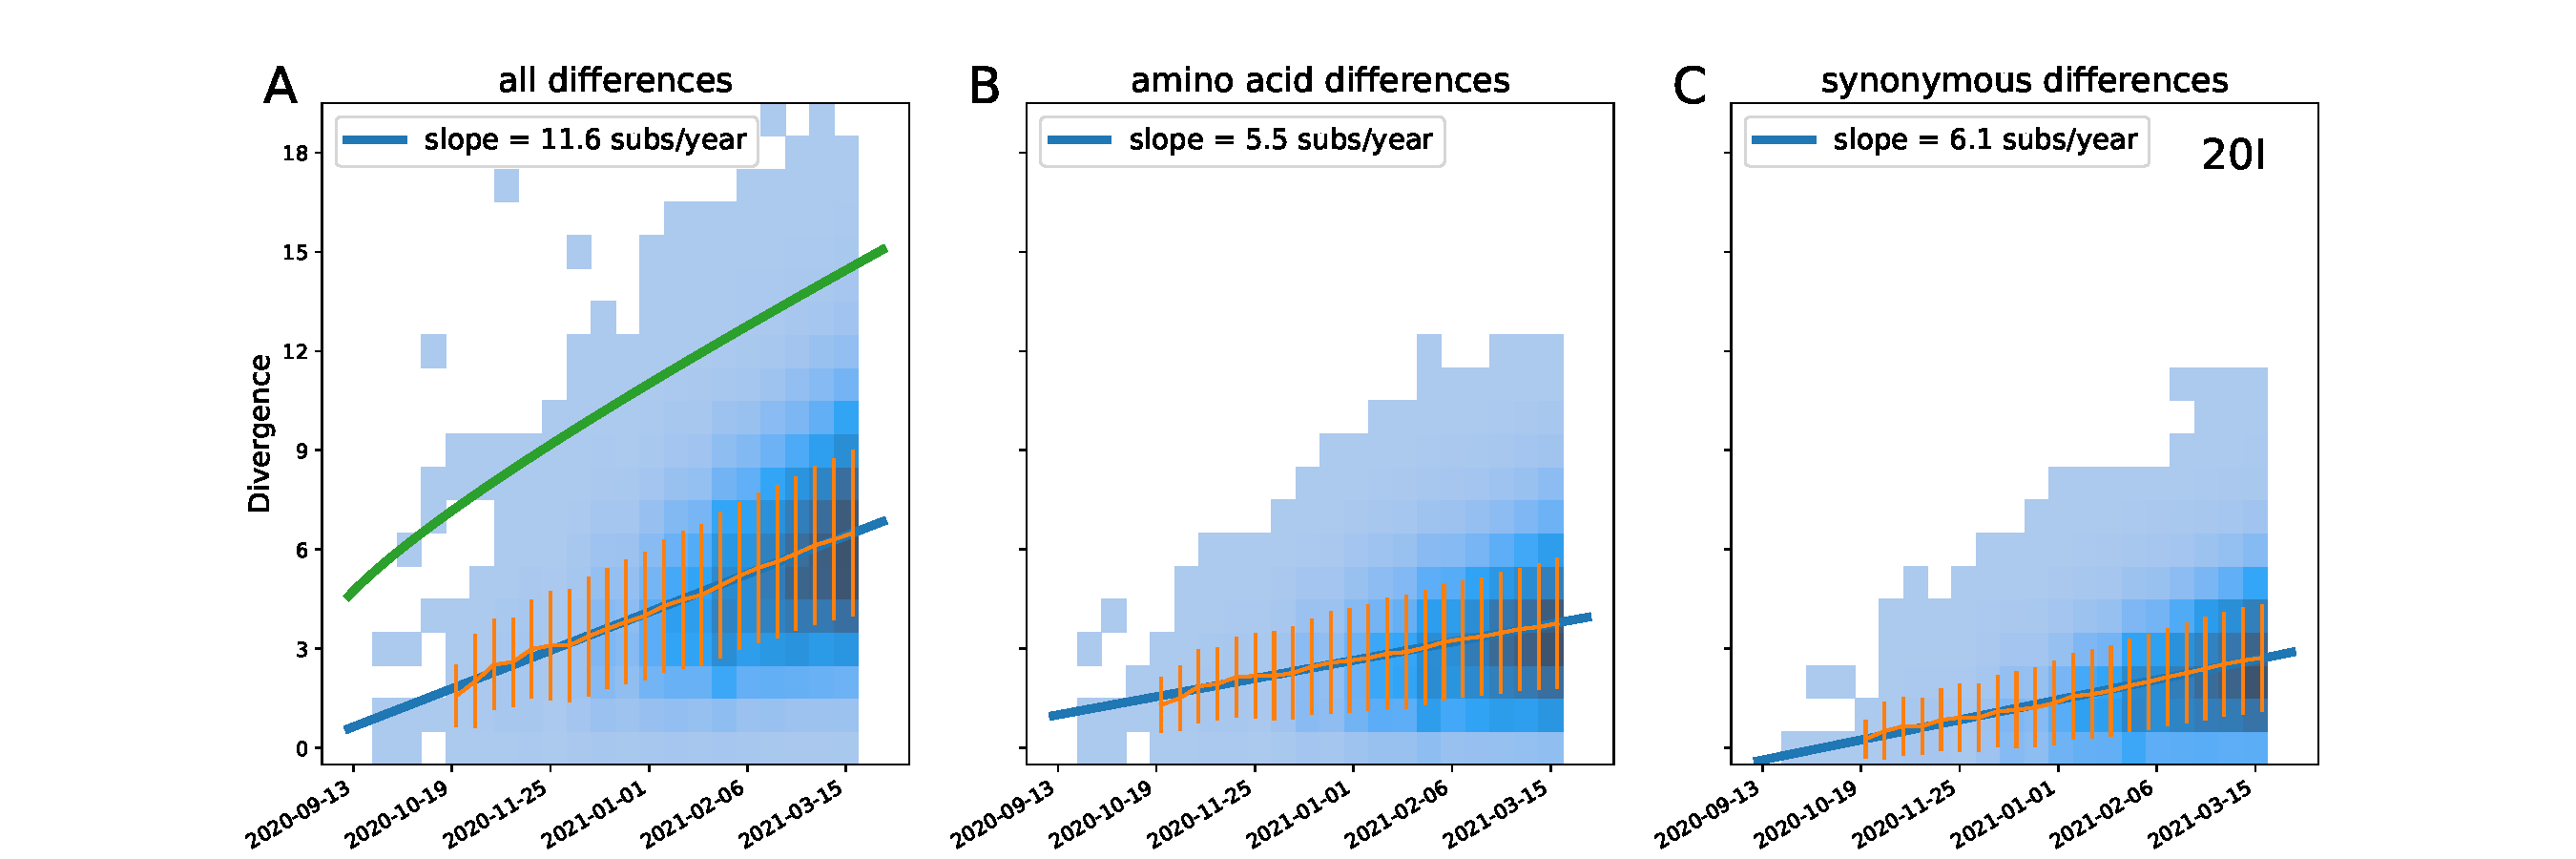
\includegraphics[width=\textwidth]{figures/rtt/20I_rtt.pdf}
    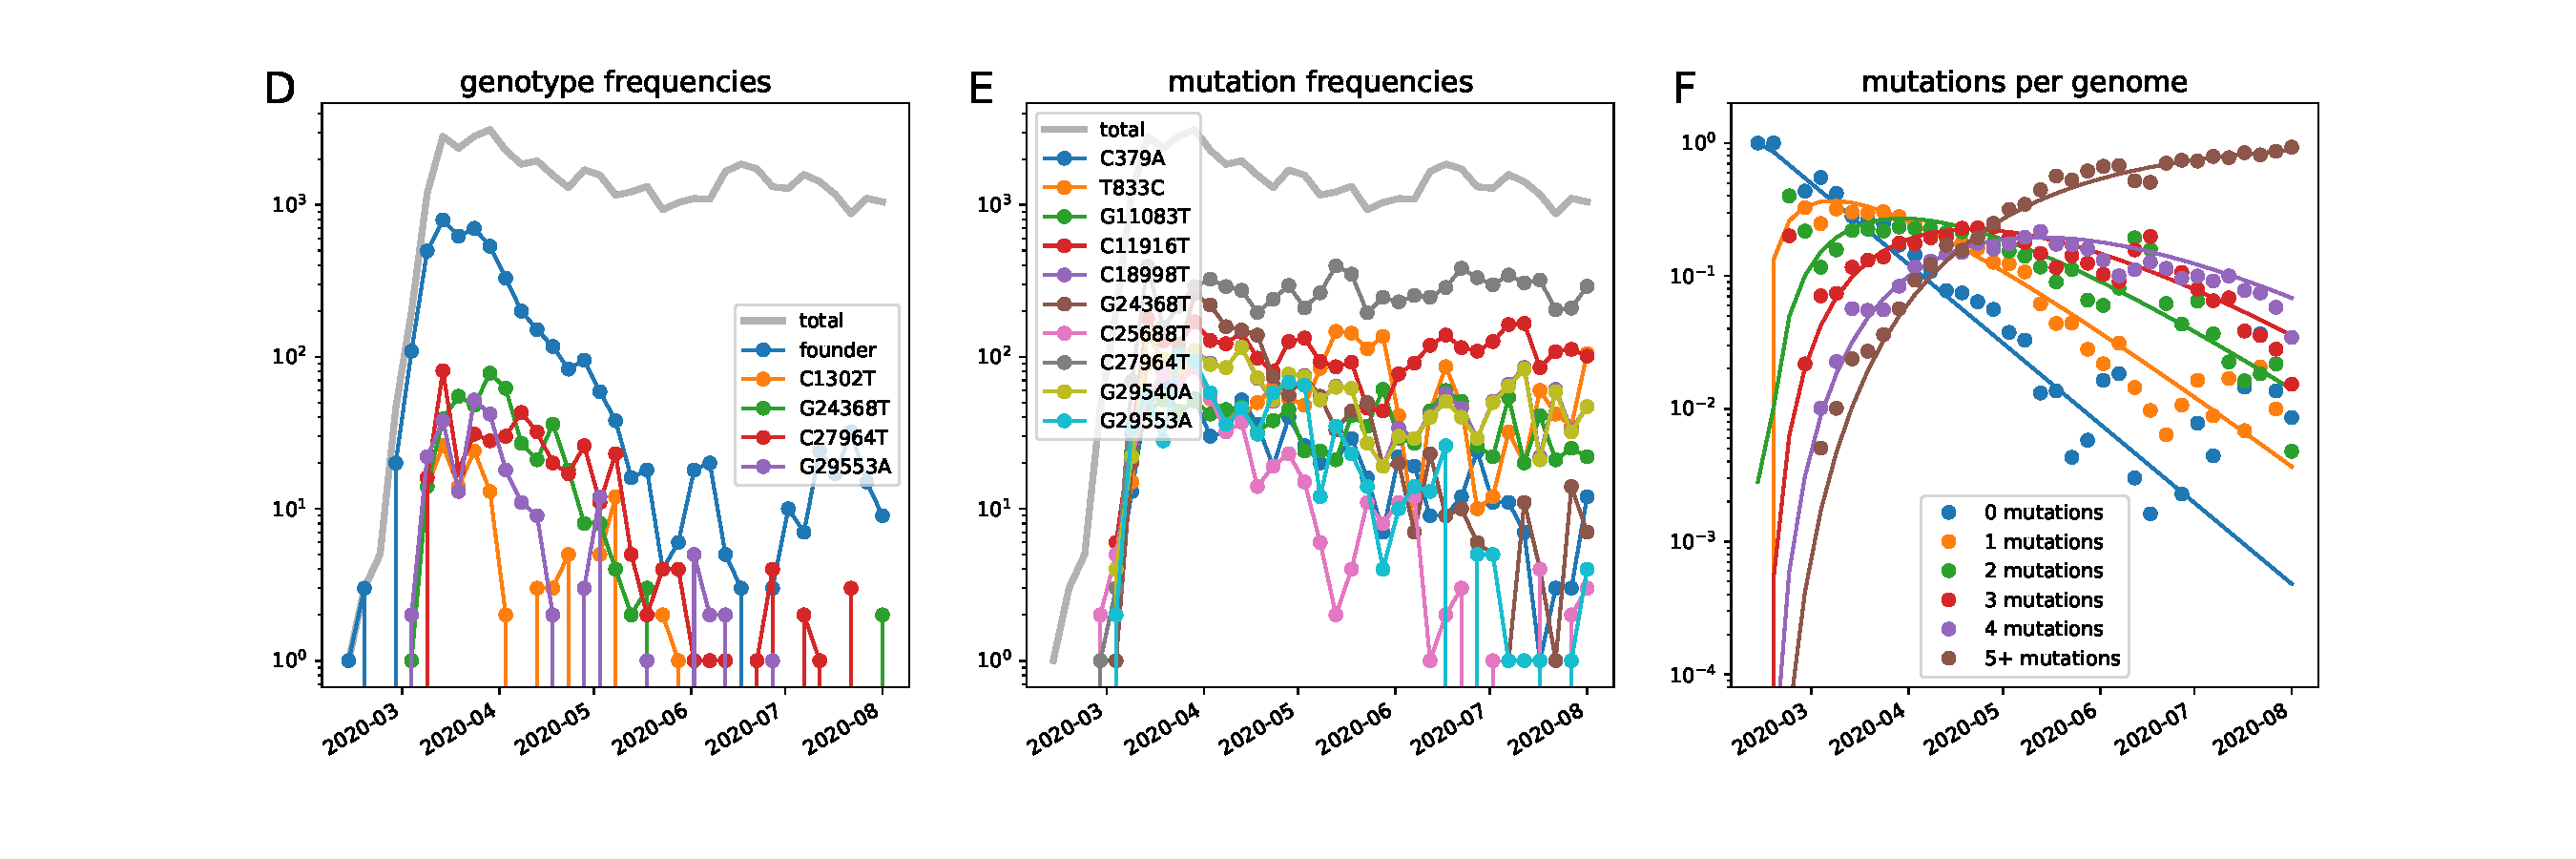
\includegraphics[width=\textwidth]{figures/counts/20C_counts.pdf}
    \caption{{\bf Within-clade divergence increases linearly with time.} Top: Each panel shows the number of within-clade mutations (total (A), amino acid changing (B), synonymous (C)) as a function of time.
    The green line in panel A indicates the divergence cut-off, panels B\&C only show sequences that pass the divergence filter. Each panel also shows mean $\pm$ standard deviation and a weighted linear fit. Analogous figures for all clades considered are included in the appendix.
    Bottom: Panels D and E show the prevalence of specific genotypes (D) and specific mutations (E). In the case shown, the founder genotype initially dominates and no daughter genotype or mutation dominate. Panel F shows a Poisson model fit to the breakdown of the population into genotypes with different number of mutations over time.
    \label{fig:within_clade}}
\end{figure*}

\section*{Results}

Evolutionary rates and divergence times are typically estimated using phylogenetic frameworks for heterochronously sampled sequences.
These methods, however, can not handle the volume of SARS-CoV-2 data available and data have to be dramatically down-sampled.
Furthermore, phylogenetic methods impose an hierarchical structure on the data and are thus very sensitive to problematic sequences or metadata: Any problematic sequence can fatally distort the analysis, in particular if placed early in tree.

To circumvent many of the above mentioned problems and still use the majority of the available data, we use a combination of automated filtering and simple robust approaches to analyze the evolutionary patterns.
We first use Nextclade \citep{aksamentov_nextclade_2021} to assign all sequences to one of the Nextstrain clades \citep{hadfield_nextstrain_2018} and analyze each clade separately.
Sequences belonging to recombinant lineages are excluded.
These clades represent well defined groups of sequences with little non-vertical evolution within them.
Furthermore, we define a ``founder'' genotype for each clade and exclude any sequence that does not have the full set of mutations relative to the reference sequence Wuhan/Hu-1.
This founder sequence is manually curated for each clade considered.
This filtering removes most incomplete sequences as well as sequences where amplicon drop-out are back-filled with reference sequence.
For this reduced set of sequences, we determine the mutations they carry on top of the founder genotype to analyze diversification and divergence within the clade.
The latter step is done for nucleotide changes as well as for amino acid changes.

Within each clade, the number of mutations is expected to increase linearly in time and the variation around this mean would, in an ideal case, obey Poisson statistics.
For the majority of sequences, this is approximately true, but some problematic sequences are many more mutations than expected.
To exclude these outliers, we perform a simple linear regression of the number of ``intra-clade'' mutations against time and remove sequences whose deviation from the linear fit exceeds twice the expected variance by 3.


After removing these outliers, we now bin the data by calendar week and determine the mean and standard deviation in each bin.
Evolutionary rate and putative emergence date of the variant are then estimated by weighted linear regression where each bin is weighted with the fourth root of the number of sequences in the bins.
The exact functional form of this weighing does not have a big influence on the results, but a sublinear weighing helps to counter the large variation in sequencing effort across countries and the natural imbalance due to the fact that few sequences are available early.

Due to shared ancestry, divergences of sequences are not independent data points and a regression against time is not suited to estimate evolutionary rates in general.
In particular, confidence intervals are difficult to obtain.
However, in the case of rapidly expanding variants we typically observe a large number of independent lineages emanating from one or several basal polytomies.
Along each of these lineages, mutation accumulation is independent and divergence increase allows to estimate the rate robustly.
Fig.~\ref{fig:within_clade} shows the increasing intra-clade divergence for clade 20C, corresponding to a large clade that emerged in early 2020 that was common in North America and Scandinavia.
Both synonymous and non-synonymous within-clade average divergence increases linearly over time allowing for a robust estimate of the rate.


A simple model for diversity in a growing variant is a super-critical branching process with growth rate $\alpha$ and an embedded mutation process.
Offspring of genomes with $i$ mutations contain $i+j$ mutations, where $j$ is a Poisson distributed number with mean $\mu t$ (mutation rate $\mu$ and generation time $t$).
The probability that offspring genomes are identical to their parents is $u = 1-e^{-\mu t}$, which for a generation time of $t=5days$ and a rate of $\mu = 15/year$ evaluates to $u\approx 0.2$.

When considering a rapidly growing well sampled outbreak, typically a single founder genotype will give rise to a large number of daughter lineages that evolve independently.
In this case, the diversification processes is robustly described by its mean
Since the above branching process is linear, the mean number of cases $n$ will increase exponentially with rate $\alpha$, while the number of genomes with $i$ mutations relative to the founder $m_i$ grows with rate $\alpha - u$ per generation:
\begin{equation}
    \begin{split}
        \frac{dn}{dt} &= \alpha n \\
        \frac{dm_0}{dt} &= (\alpha - u) m_0 \\
        \frac{dm_1}{dt} &= u m_0 (\alpha - u) m_1 \\
        \frac{dm_2}{dt} &= u m_1 (\alpha - u) m_2 \\
        \cdots
    \end{split}
\end{equation}
with solution $m_i = e^{(\alpha - u)t} \frac{(ut)^i}{i!}$.
At each time the number of mutations in the population is expected to Poisson distributed with mean $ut$, while the overall number of cases is $e^{\alpha t}$ or more generally $e^{\int \alpha(t) dt}$ if growth rate or ascertainment varies over time.

For some clades, especially those that are well sampled soon after their emergence, this Poisson model is good fit to diversity accumulation and yields estimates of rates and time of origin that are compatible with the divergence regression, see Fig.~\ref{fig:within_clade}F for clade 20C.
Analogous plots for all other clades considered are included in the appendix.

In some cases, subclades do become dominant in the early stochastic dynamic.
This can result in increased within clade divergence, effectively generating an offset to diversity.
Extrapolation of the linear fit to zero divergence is thus not necessarily a good estimator of the emergence time of a variant.
For several clades 19B, 20H (Beta), 21D (Eta), 21G (Lambda), 21 (Mu), 21I (Delta), 21J (Delta), 21L (Omicron, BA.2), and 22B (Omicron, BA.5), founder like variants are a minority even in early data.

These Poisson weights of mutation numbers are again only valid if mutations accumulate along many independent lineages.
In particular, this assumption is violated if some lineages spread systematically faster than others either because of epidemiological factors or the mutations they carry.
In variant 21K (Omicron, BA.1), a sublineage with mutation $S:R346K$ might have enjoyed a transmission advantage.
A possible consequence of this advantage is visible in Supp.~Fig.~\ref{fig:21K_divergence} where genotypes with 0, 1, or 2 mutations are decaying more rapidly than those with more mutations.

\begin{figure*}
    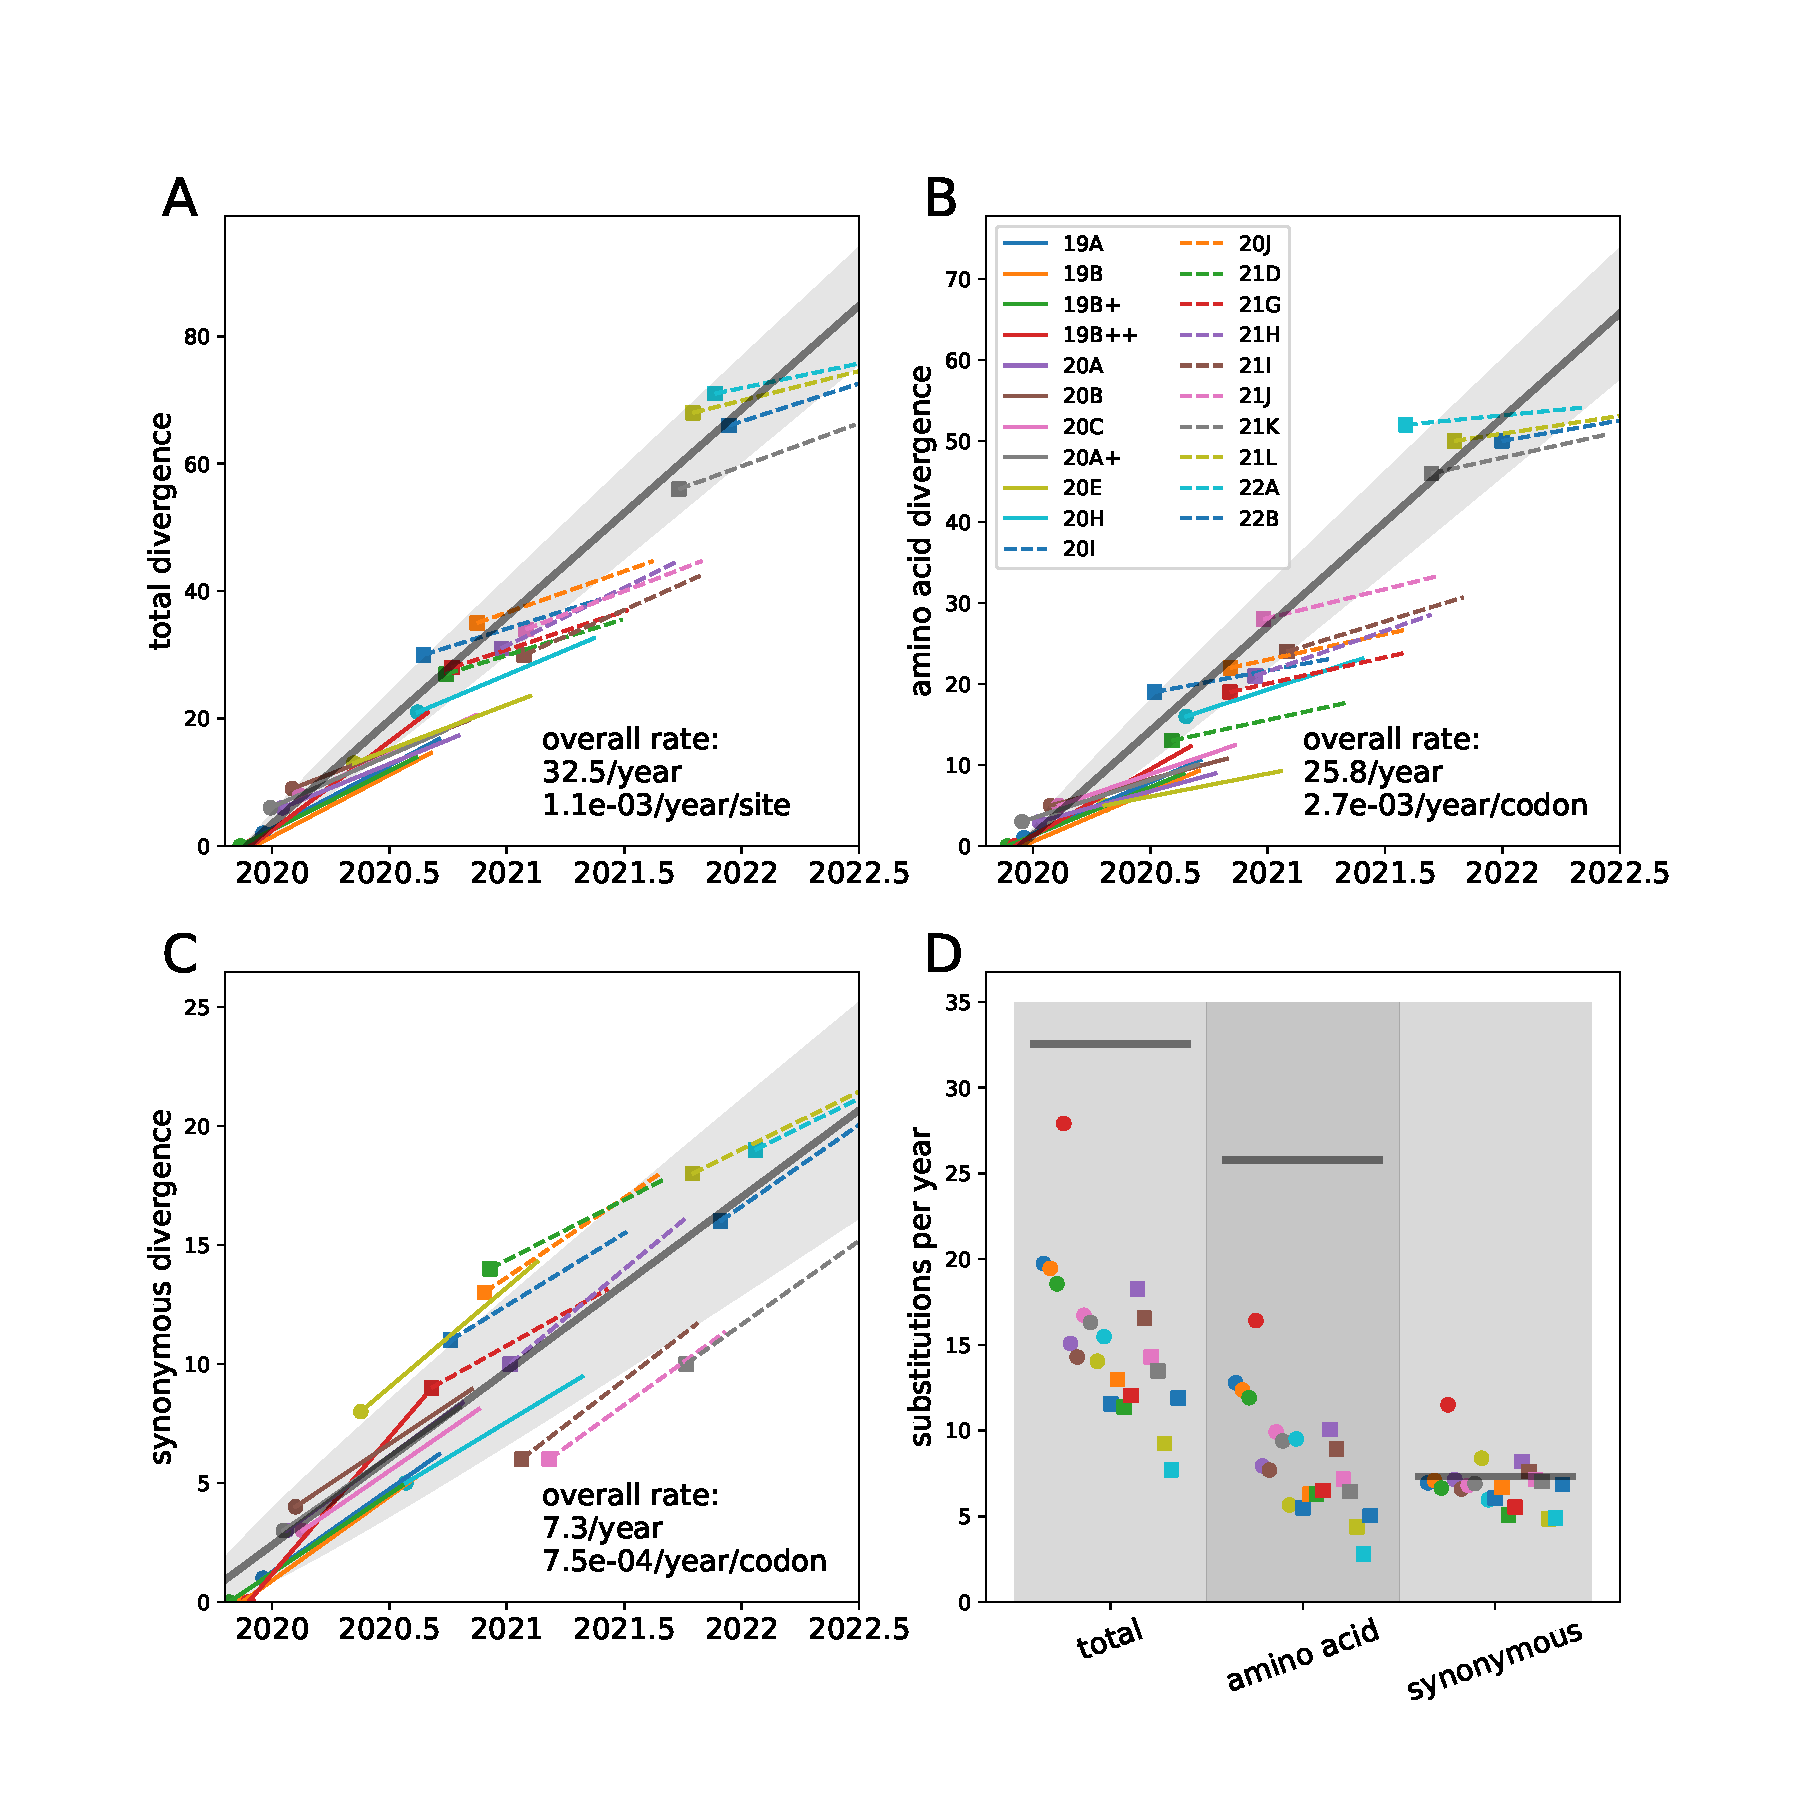
\includegraphics[width=0.8\textwidth]{figures/rate_summary.pdf}
    \caption[]{{\bf Divergence and evolutionary rates of different Nextstrain clades.} Panels A,B,\&C show the estimated divergence of the founder genotype of each clade (big dot) and the subsequent divergence trend for all nucleotide changes, amino acid changes, and synonymous changes, respectively. In addition, each panel contains a regression of the divergence of clade founders vs time (gray line).
    The standard deviation expected based on Poisson statistics is indicated as shaded area.
    Panel D summarizes the individual rate estimates (dots and squares) and compares them to the estimate inter-clade rates (gray lines).
    \label{fig:rate_summary} }
\end{figure*}

Despite these caveats, for almost all major Nextstrain clades, the average divergence increases linearly in time (similar patterns as Fig.~\ref{fig:within_clade}A-C for clade 20C) allowing us to estimate clade specific evolutionary rates for amino acid and silent changes.
These rates are summarized in Fig.~\ref{fig:rate_summary} and Tab.~\ref{tab:rates}.

Rates of synonymous change are very consistent across variants and also agree with the overall rate of synonymous changes of about 5-8 changes per genome per year, while rates of non-synonymous changes are much more variable (Fig.~\ref{fig:rate_summary}D).
Within clades, the rate of non-synonymous changes varies between 5 and 16 changes per year.
Earlier clades are estimated to have larger rates around 10-15 changes per year, while rate estimates for later clade fall  between 3 to 9 changes per year Fig.~\ref{fig:rate_progression}.
In contrast, the inter-clade non-synonymous rate exceeds 25 changes per year.

Nextstrain clades tend to be defined by long branches leading to a large polytomy.
It is thus expected that the estimated inter-clade rate exceeds the intra-clade rate purely because of this conditioning.
This effect might be particularly important early on in the pandemic where branches with as little two mutations were used to define new clades.
We thus also included composite clades 19B+, 19B++ and 20A+ containing sequences from 19A and 19B (rooted on 19B), 19A, 19B, 20A, 20B, 20C, 20D (rooted on 19B), and 20A, 20B, 20C, 20D (rooted on 20A).
The estimates for composite clades 19B+ and 20A+ are consistent with the estimates of the individual clades, while apparent rates of 19B++ are considerably higher.
The latter is due to the rapid expansion and subsequent dominance of clade 20A and its descendants which rapidly added four additional mutations \citep{korber_tracking_2020}.

\begin{table*}
\begin{tabular}{l|rrrrrr}
    \hline
    {\bf clade} &  overall rate $[y^{-1}]$ & aa rate $[y^{-1}]$ &  syn rate $[y^{-1}]$ & overall div. &  aa div. &  syn div. \\
    \hline
    19B &     19.45 &    12.37 &      7.09 &        0 &       0 &        0 \\
    19B+ &     18.51 &    11.87 &      6.64 &        0 &       0 &        0 \\
    19B++ &     28.17 &    16.32 &     11.84 &        0 &       0 &        0 \\
    19A &     19.75 &    12.79 &      6.96 &        2 &       1 &        1 \\
    20A &     15.59 &     8.33 &      7.26 &        6 &       3 &        3 \\
     20B &     14.17 &     7.64 &      6.53 &        9 &       5 &        4 \\
     20C &     16.43 &     9.63 &      6.79 &        8 &       5 &        3 \\
    20A+ &     17.16 &     9.76 &      7.40 &        6 &       3 &        3 \\
     20E &     13.88 &     5.84 &      8.04 &       13 &       5 &        8 \\
     20H &     15.46 &     9.50 &      5.96 &       21 &      16 &        5 \\
     20I &     11.78 &     5.72 &      6.06 &       30 &      19 &       11 \\
     20J &     12.91 &     6.29 &      6.62 &       35 &      22 &       13 \\
     21D &     11.36 &     6.29 &      5.07 &       27 &      13 &       14 \\
     21G &     12.03 &     6.51 &      5.51 &       28 &      19 &        9 \\
     21H &     18.24 &    10.05 &      8.19 &       31 &      21 &       10 \\
     21I &     16.26 &     8.63 &      7.63 &       30 &      24 &        6 \\
     21J &     13.26 &     6.91 &      6.36 &       34 &      28 &        6 \\
     21K &     14.04 &     6.55 &      7.49 &       56 &      46 &       10 \\
     21L &      9.40 &     4.12 &      5.28 &       68 &      50 &       18 \\
     22A &      8.07 &     2.84 &      5.23 &       71 &      52 &       19 \\
     22B &     12.06 &     4.96 &      7.10 &       66 &      50 &       16 \\
         \hline
    \end{tabular}
\caption{{\bf Evolutionary rates estimates from root-to-tip regressions for overall nucleotide changes, amino acid changes, and synonymous changes.}
    The last three columns give the distances of the clade founder sequence from putative MRCA of SARS-CoV-2.
\label{tab:rates}}
\end{table*}

\begin{figure}
    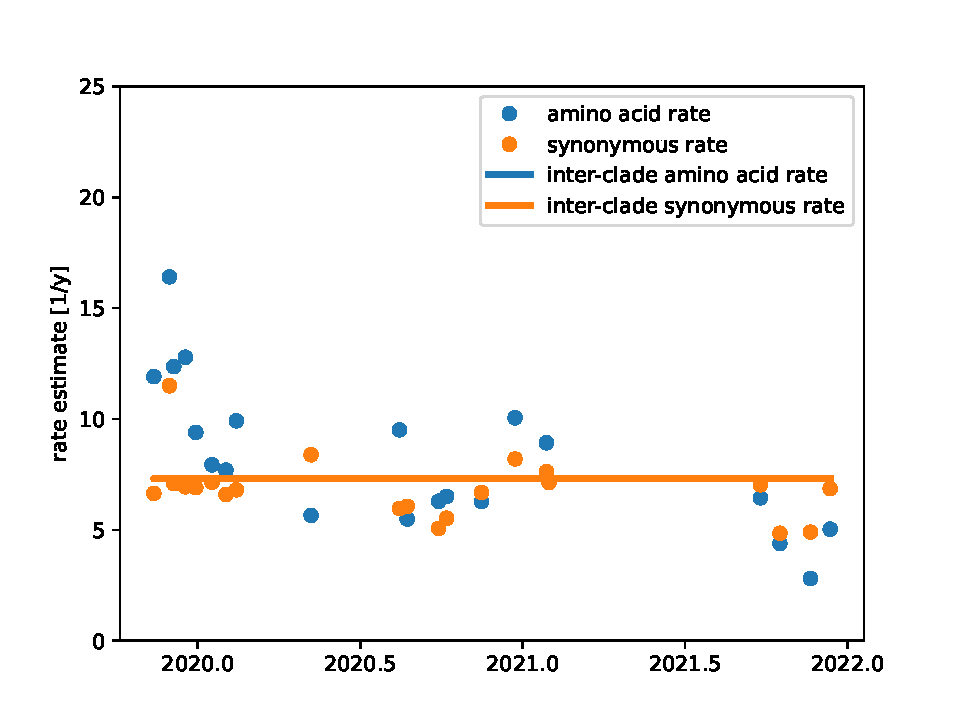
\includegraphics[width=0.5\textwidth]{figures/rate_progression.pdf}
    \caption{{\bf Divergence and evolutionary rates of different Nextstrain clades over time.} Synonymous rates estimates are stable in time and fluctuate around the rate estimates for between clades. Non-synonymous rate estimates are highest for clades 19A - 20C.
    \label{fig:rate_progression} }
\end{figure}

% The apparently higher non-synonymous rate suggests that at the beginning a large fraction of amino acid changes were beneficial to viral replication, not just the D614G mutation in the spike protein \citep{korber_tracking_2020}.
% This applies both to the changes within clades that were ultimately displaced by more successful variants, and inter-variant changes where the fraction of adaptive changes is even higher.



\section*{Purifying selection and mutation tolerance}

Above, we found that the rate of synonymous mutations is comparable within and between clades without any striking signal of temporal variation.
This is expected, as synonymous positions are rarely a locus of adaptation and tend to have a small effects on fitness in large parts of the genomes of RNA viruses \citep{zanini_vivo_2017} (outside of specific regions with important RNA elements or splice sites).
To assess the level of constraint on the SARS-CoV-2 genome, we made use of the ``rare mutations'' annotation by Nextclade.
Nextclade attaches each sequence to a reference tree and determines by which mutations it differs from the attachment point.
For each Pango lineage (as determined by Nextclade) \citep{rambaut_dynamic_2020,aksamentov_nextclade_2021}, we count how often these ``rare mutations'' (including reversions to reference) are observed, normalize this against the relative rate of mutation away from the ancestral nucleotide (see Supp.~Fig.~\ref{fig:mutation_distribution}), and use this as a proxy for mutational tolerance.

Simply splitting mutations into those that occur in 1st, 2nd, and 3rd positions of codons already reveals strong signatures of purifying selection, see Fig.~\ref{fig:fitness_costs}.
Between 15-20\% of positions at first and second codons show almost no variation, while half of these sites are less variable then the most constrained 10\% of third positions.
The median of variation at 3rd position is more than double that at other 1st and 2nd positions.

When split by open reading frame (see Supp.~Fig.~\ref{fig:fitness_costs_supp} and \ref{fig:fitness_landscape}), the most constrained are \emph{ORF1b} and \emph{M}, while \emph{ORF3a, ORF6, ORF7a, ORF7b}, and \emph{ORF8} show little evidence of constraint, consistent with frequently observed stop-mutations in these genes.
\emph{N} shows an intermediate pattern, possibly reflecting its mix of structured and unstructured regions.
Rare variation at 3rd positions is very comparable between genes.
Only \emph{E} shows slightly less variation at 3rd positions than other genes with a notable dip in the middle of the gene around codon 35.



\begin{figure}
    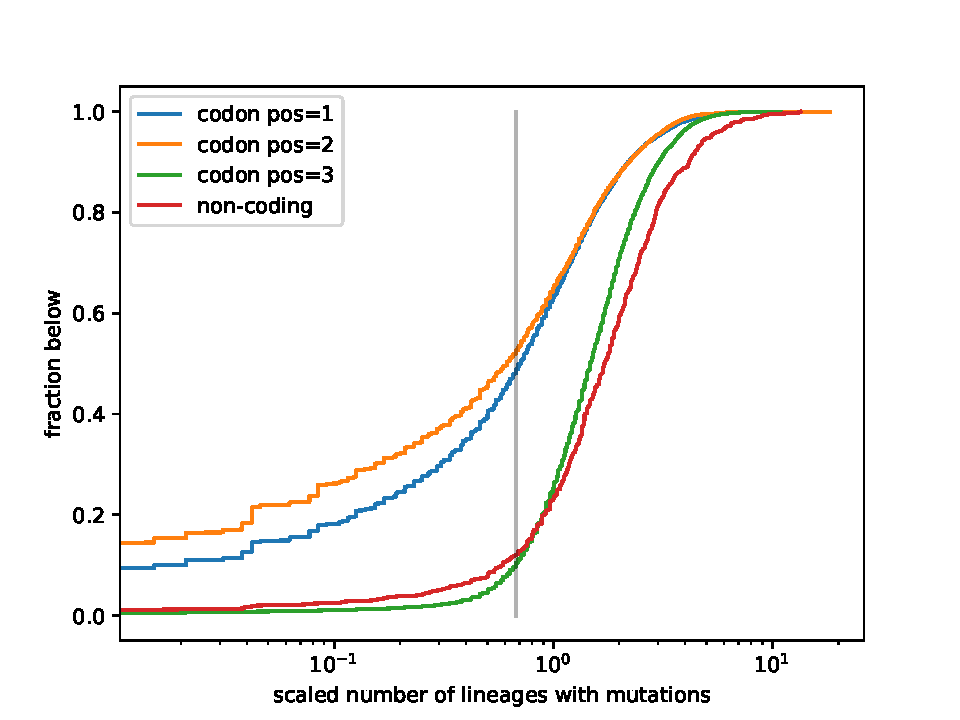
\includegraphics[width=0.5\textwidth]{figures/fitness_cost.pdf}
    \caption{{\bf Constraints on SARS-CoV-2 mutations.}
    Almost all 3rd codon positions tolerate mutations, while 1st and 2nd positions are strongly constrained.
    About half of the 1st and 2nd codon positions are less variable than the most constrained 10\% of 3rd positions (gray line).
    \label{fig:fitness_costs}}
 \end{figure}

 \begin{figure*}[tb]
    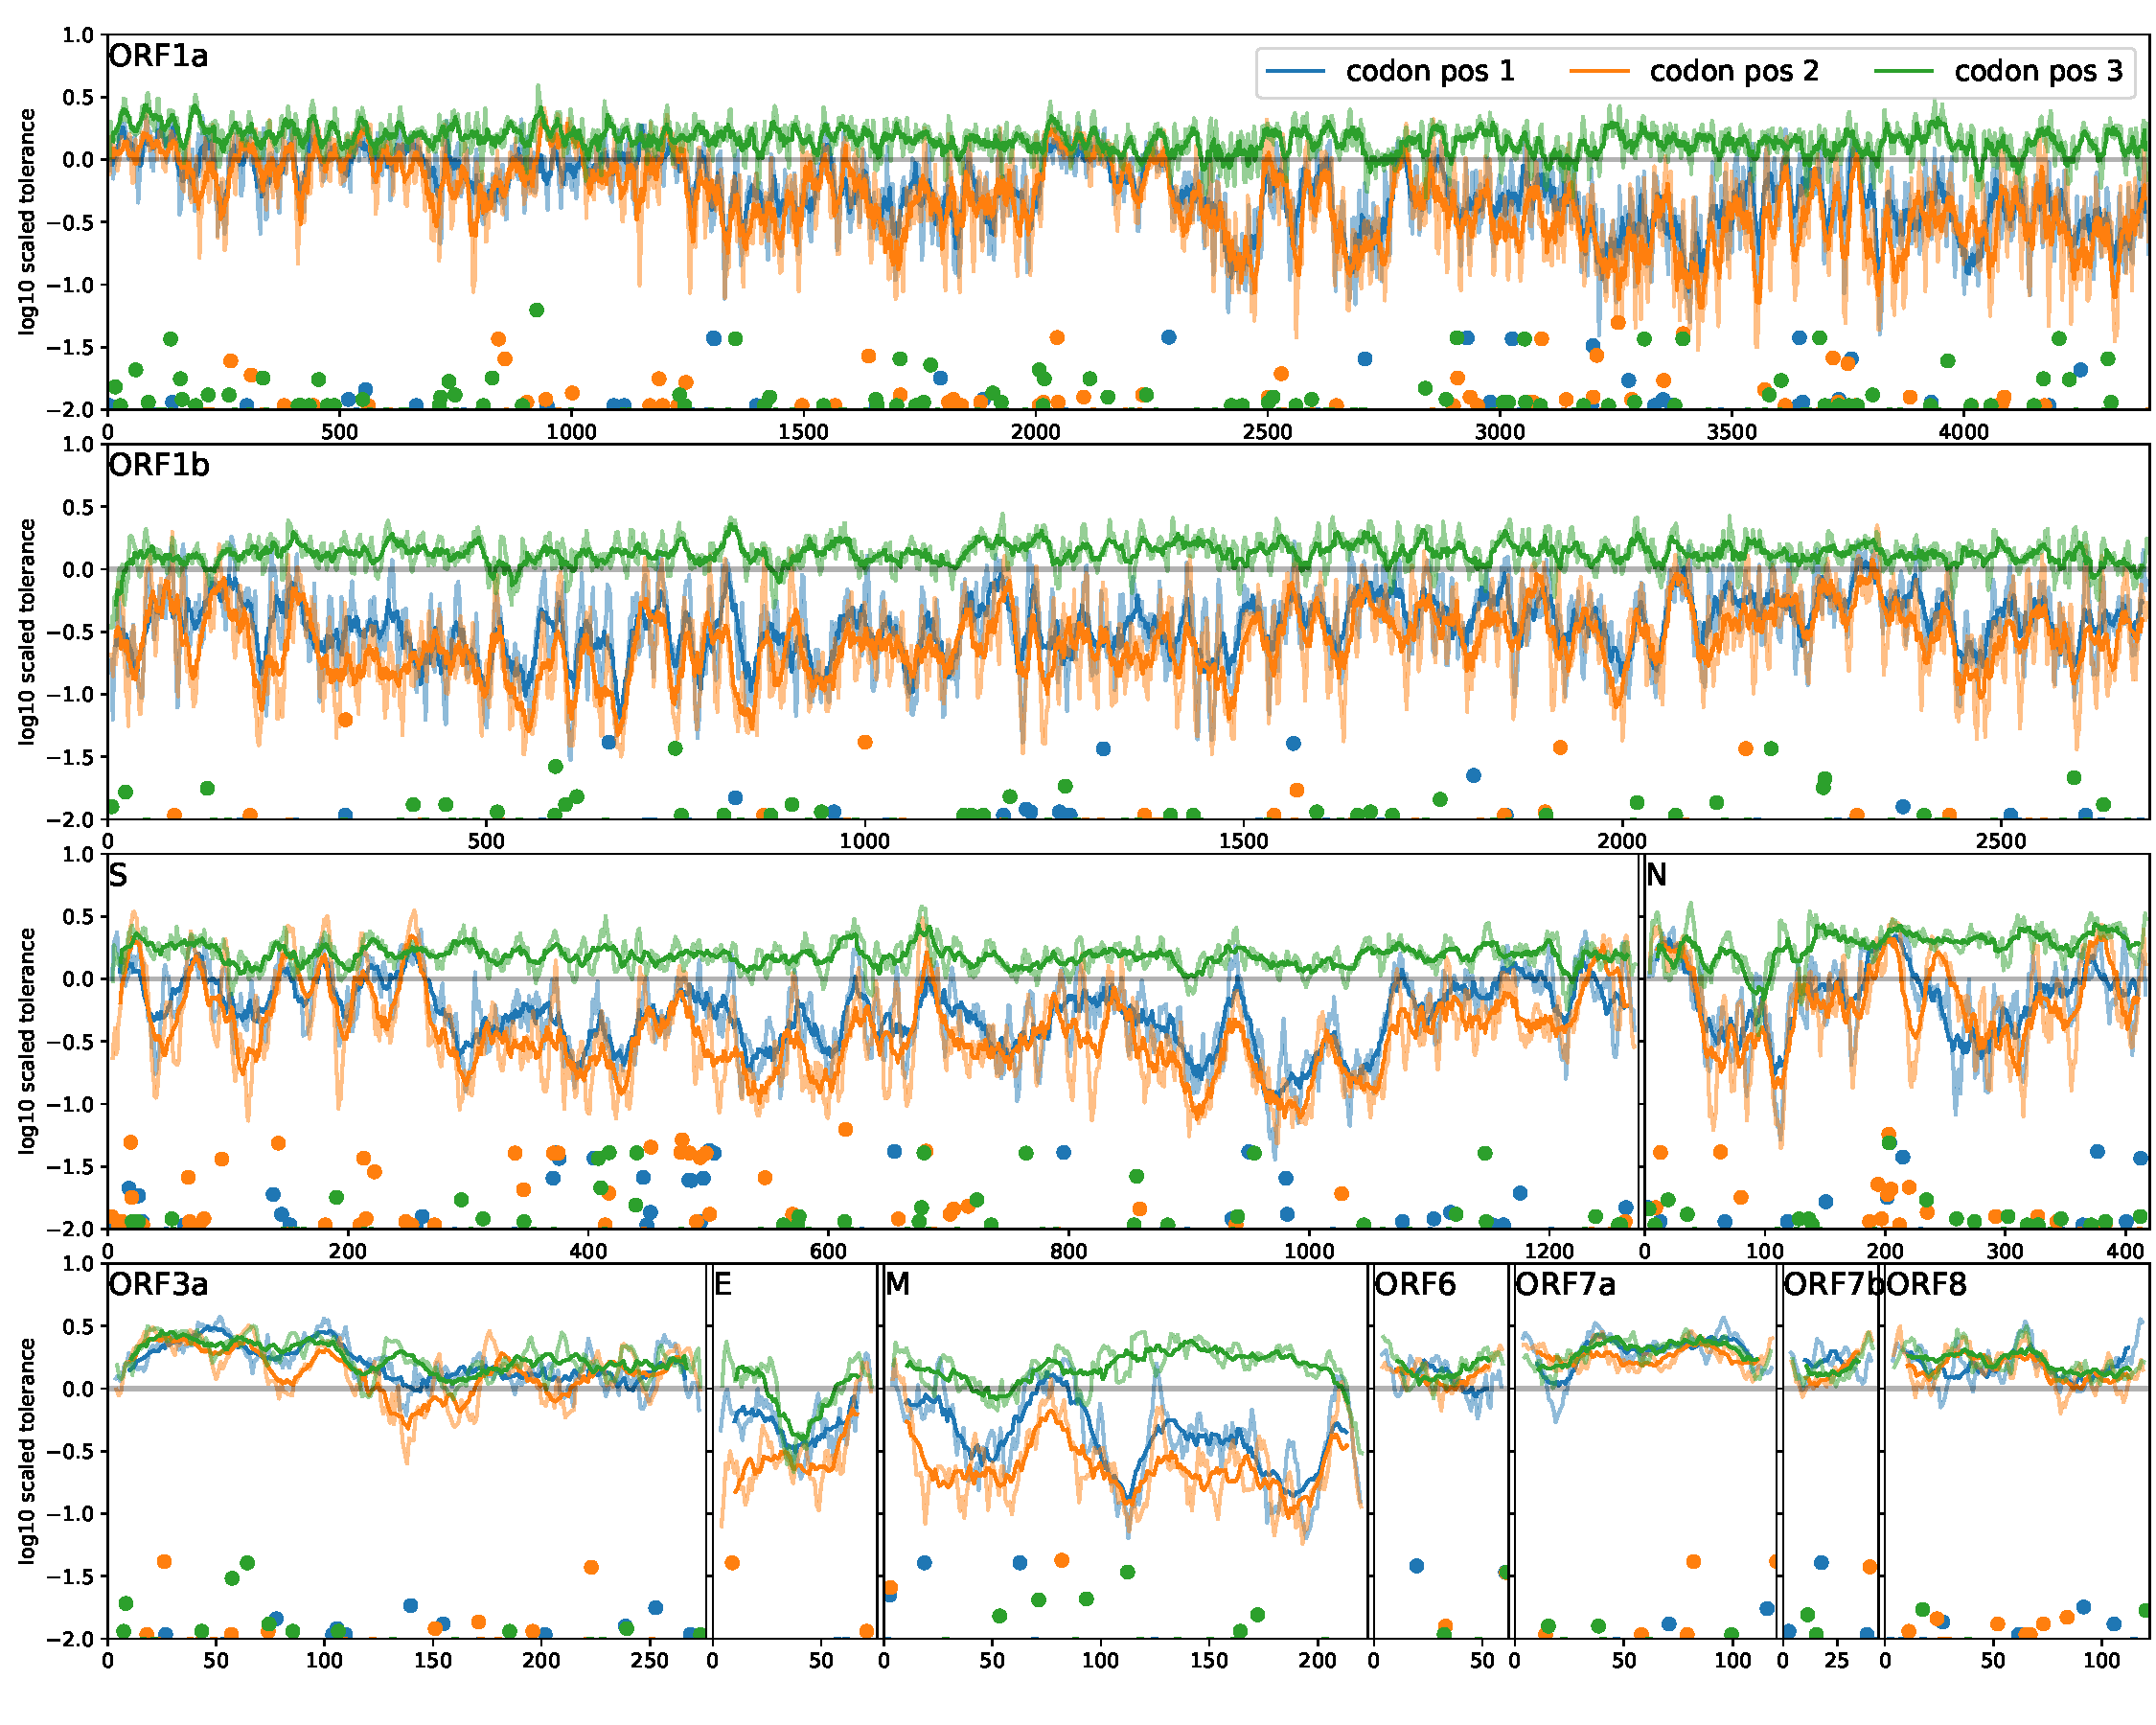
\includegraphics[width=\textwidth]{figures/fitness_landscape.pdf}
    \caption{{\bf Landscape of selective constraint along the SARS-CoV-2 genome.}
    Solid lines show sliding window smoothing of estimated mutational tolerance at 1st, 2nd, and 3rd positions for a window size of 20 and 7 (faint lines) sites.
    The markers below the lines are a qualitative indication of variable positions across SARS-CoV-2 diversity.
    \label{fig:fitness_landscape}}
 \end{figure*}

\section*{Discussion}
The inferred evolutionary rate of RNA viruses often decreases with the time scale across which is it estimated \citep{wertheim_purifying_2011,ghafari_prisoner_2021}.
This effect is particularly pronounced at the beginning of an outbreak following a host switch and has been attributed to methodological issues and incomplete purifying selection leading to inflated measures of diversity \citep{meyer_time_2015,ghafari_purifying_2022}.
In addition to segregating deleterious mutations, early viral evolution after a host switch will also be affected by anomalously fast adaptive evolution as a dramatic change in environment, i.e.~a host switch, likely results in many mutations that increase fitness, though sometimes these better adapted states require multiple epistatically interacting mutations \citep{martin_emergence_2021}.
Such transient increases in the rate of adaptation are common in experimental evolution \citep{elena_virus_2007}.

Since we analyzed evolution within short lived clades of SARS-CoV-2 over a span of 6 month, purifying selection has comparable efficiency for all clades.
Sequencing artefacts are expected to increase divergence at all time points or decrease with time as sequencing workflows improve.
Nevertheless, the estimated non-synonymous evolutionary rate of clades circulating in late 2019 and early 2020 is about twice as high as that of clades in 2021 and 2022, while the synonymous rate does not change (see Fig.~\ref{fig:rate_summary} and Table \ref{tab:rates}).
One possible explanation is that the early evolutionary rate of SARS-CoV-2 was inflated by adaptive evolution.

Most of this apparent acceleration of within-variant evolution ceased in mid 2020 and even early variants like 20E accumulated non-synonymous changes at a rate of about 6 per year instead of 12.
By that time, the number of non-synonymous mutations was SARS-CoV-2 small (5 in the case of 20E) and given what is observed in subsequent variants, it is implausible that this small change would have exhausted the pool of beneficial mutations.
However, the different replication and transmission kinetics of variants with S:D614G might mean that virus is operating closer to the maximal capacity at which cells can produce virions and the strength of selection is generally reduced.
Such ``diminishing return'' epistasis as been observed in experimental evolution with yeast \citep{kryazhimskiy_global_2014}.
Differences in diversification of SARS-CoV-2 with and without the S:D614G mutation where also observed in evolution experiments \citep{amicone_mutation_2022}, who concluded that these differences were not due to a change in base line mutation rate.

An evolutionary rate of 6 synonymous changes at around 9000 positions per year corresponds to a per-site mutation rate of $6.6\times 10^{-4}$ per site and year or $1.8\times 10^{-6}$/day, slightly higher than the estimated base-line mutation rate of $1.3\times 10^{-6}$/day \citep{amicone_mutation_2022}.
The overall rate in variants starting with 20E is in the range of 9-16 changes per year, corresponding to a per site rate of $3 - 5\times 10^{-4}$/site and year, consistent with recent estimates by \citet{hill_origins_2022} and \citet{tay_emergence_2022}.

When considering only the putative founder genotype and date of origin of each variant, all variants so far are compatible with a back-bone evolutionary rate of 32 changes per year, corresponding to an per site rate of around $10^{-3}$/site/year (see Fig.~\ref{fig:rate_summary}).
This rate is a composite of episode of cryptic accelerated evolution (probably in chronically infected individuals), and regular transmission chains of acute infections.
This is thus lower than the branch specific rates estimated by \citet{hill_origins_2022} and \citet{tay_emergence_2022}.
However, all clades and variants are compatible with a single ``back-bone'' molecular clock without postulating significant differences in the emergence of different variants.
This observation of course does not rule out that different clades and variants emerged in qualitatively different ways.

By analyzing the rate mutations that spread only on short times scales within fine-grained Pango lineages, we estimated the level of constraint on different parts of the SARS-CoV-genome.
The great majority of 3rd positions in codons at which  most mutations are synonymous do not show strong signatures of conservations.
The major open reading frames ORF1ab, S, N, E, M show clear signatures of purifying selection with around 50\% of sites being more constrained than the most constrained 10\% of 3rd positions.
This result is consistent with similar analysis in HIV that also show little fitness costs for most synonymous mutations, while half of non-synonymous mutations are so deleterious that they are not even observed on short times scales \citep{zanini_vivo_2017}.
The remaining ORFs show little global signal of constraint and 1st and 2nd positions are as variable as 3rd positions (see Fig.~\ref{fig:fitness_costs}).
Only a few regions show a clear signal of conservation at 3rd positions, notably a central region of \emph{E} and the ribosome slippage region at the beginning of \emph{ORF1b}.

The heterogeneity in evolutionary rates and the combination of adaptive evolution, approximately neutral mutations, and purifying selection complicate the interpretation of phylodynamic analysis, which typically assumes that the mutation process is independent of the spread and epidemiology and that different sites evolve independently.
These assumptions are (approximately) true for neutral mutations that occur along every lineage with the same rate.
Deleterious mutations are relatively straightforward to account for: Strongly deleterious mutations don't spread and are only observed on terminal branches, similar to sequencing errors.
Weakly deleterious mutations can spread, but lineages that carry them tend to be short-lived.
A spectrum of mutations with different deleterious effects leads to time dependent effective evolutionary rates \citep{wertheim_purifying_2011}.

Adaptive evolution, however, is much harder to account for properly.
Since the number of sites that allow beneficial mutations is small, adaptive evolution tends to be very stochastic -- it is not the typical events, but the rare and extreme events that determine the course of adaptive evolution.
Unlike neutral evolution, the rate of adaptive evolution depends on the population size, stochastic nature of the transmission process, the environment, and previous adaptation.



\bibliography{bib}
%\appendix
\section*{Supplementary figures}

\setcounter{figure}{0}
\renewcommand{\figurename}{Figure S}
\setcounter{table}{0}
\renewcommand{\tablename}{Table S}


\begin{figure}[h]
    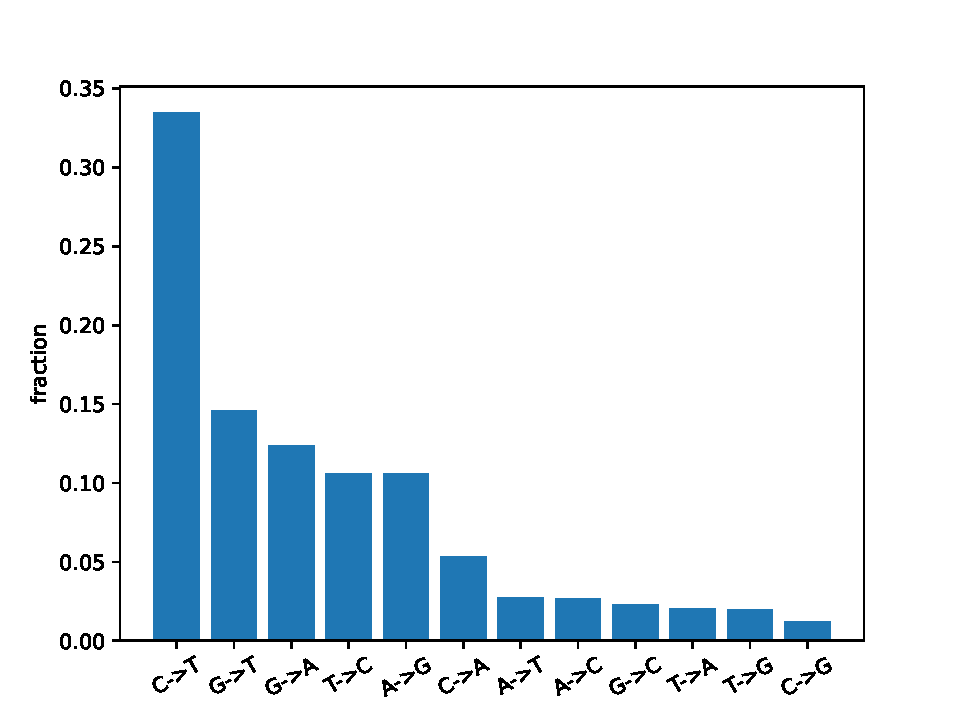
\includegraphics[width=0.5\textwidth]{figures/mutation_distribution.pdf}
    \caption{{\bf The relative rate of different mutations in SARS-CoV-2.}
    These rates are measured from rare low frequency mutations probably subject to little purifying selection.
    \label{fig:mutation_distribution}}
\end{figure}

\begin{figure}[h]
    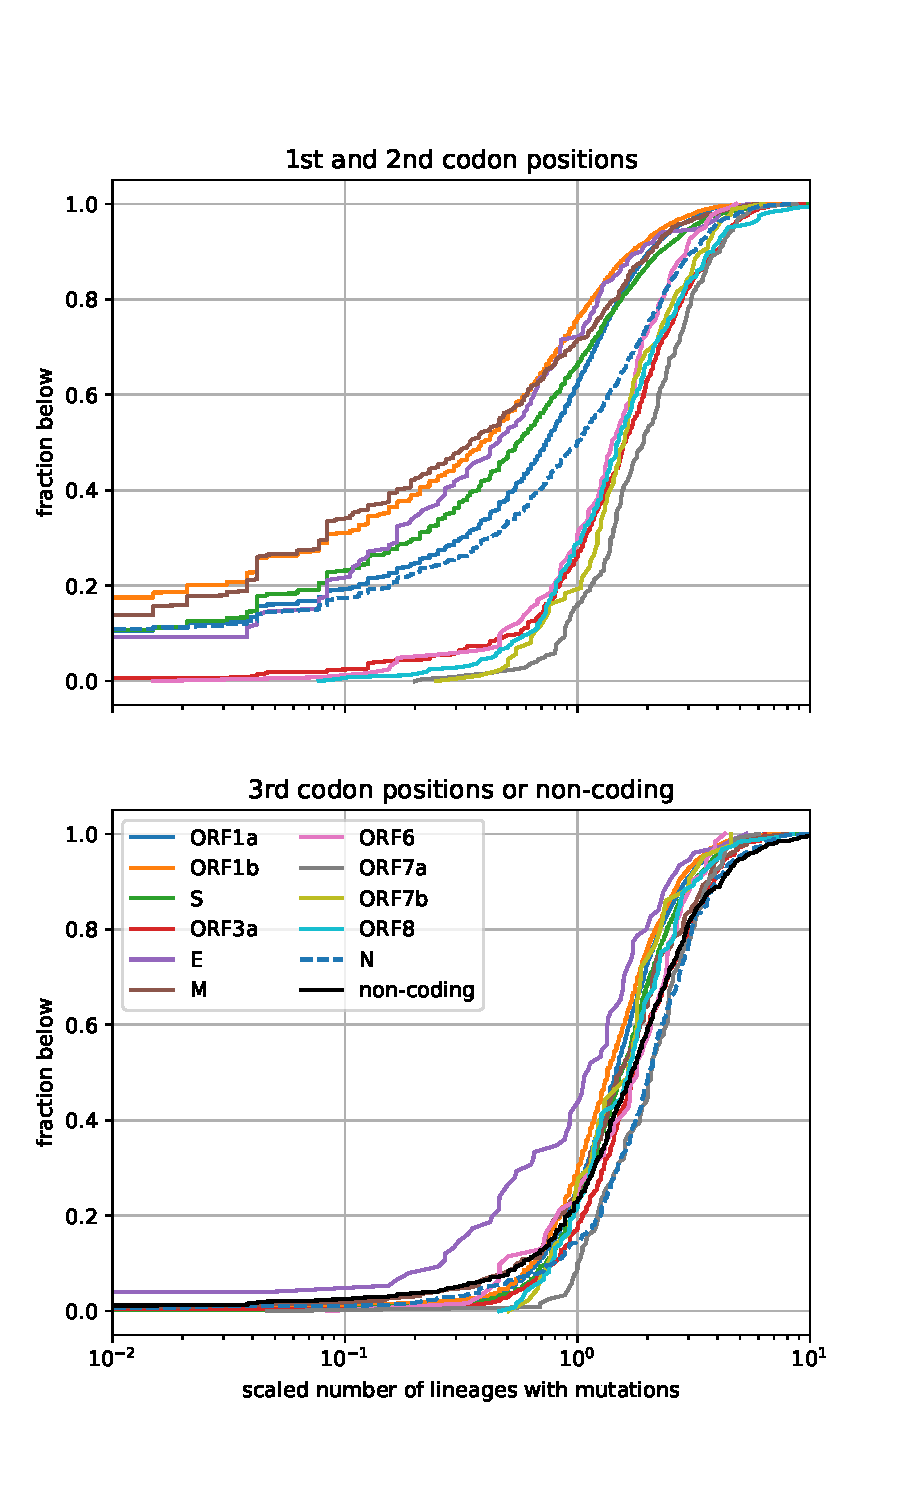
\includegraphics[width=0.5\textwidth]{figures/fitness_cost_by_gene.pdf}
    \caption{{\bf Constraints on SARS-CoV-2 mutations by gene.}
    The top panel quantifies constraint at 1st and 2nd positions in codons of open reading frames.
    The bottom panel show the analogous distributions at 3rd codon positions.
    The latter distributions are very similar across genes, with only \emph{E} showing somewhat less variation.
    In contrast, mutation tolerance at 1st and 2nd positions differs markedly between genes.
    In ORF3a, ORF6, ORF7a, ORF7b, and ORF8 the distribution of mutations at 1st and 2nd positions is very similar to the distribution at 3rd positions, while the remaining genes show clear signs of constraint.
    \label{fig:fitness_costs_supp}}
 \end{figure}

 \begin{figure}[tb]
    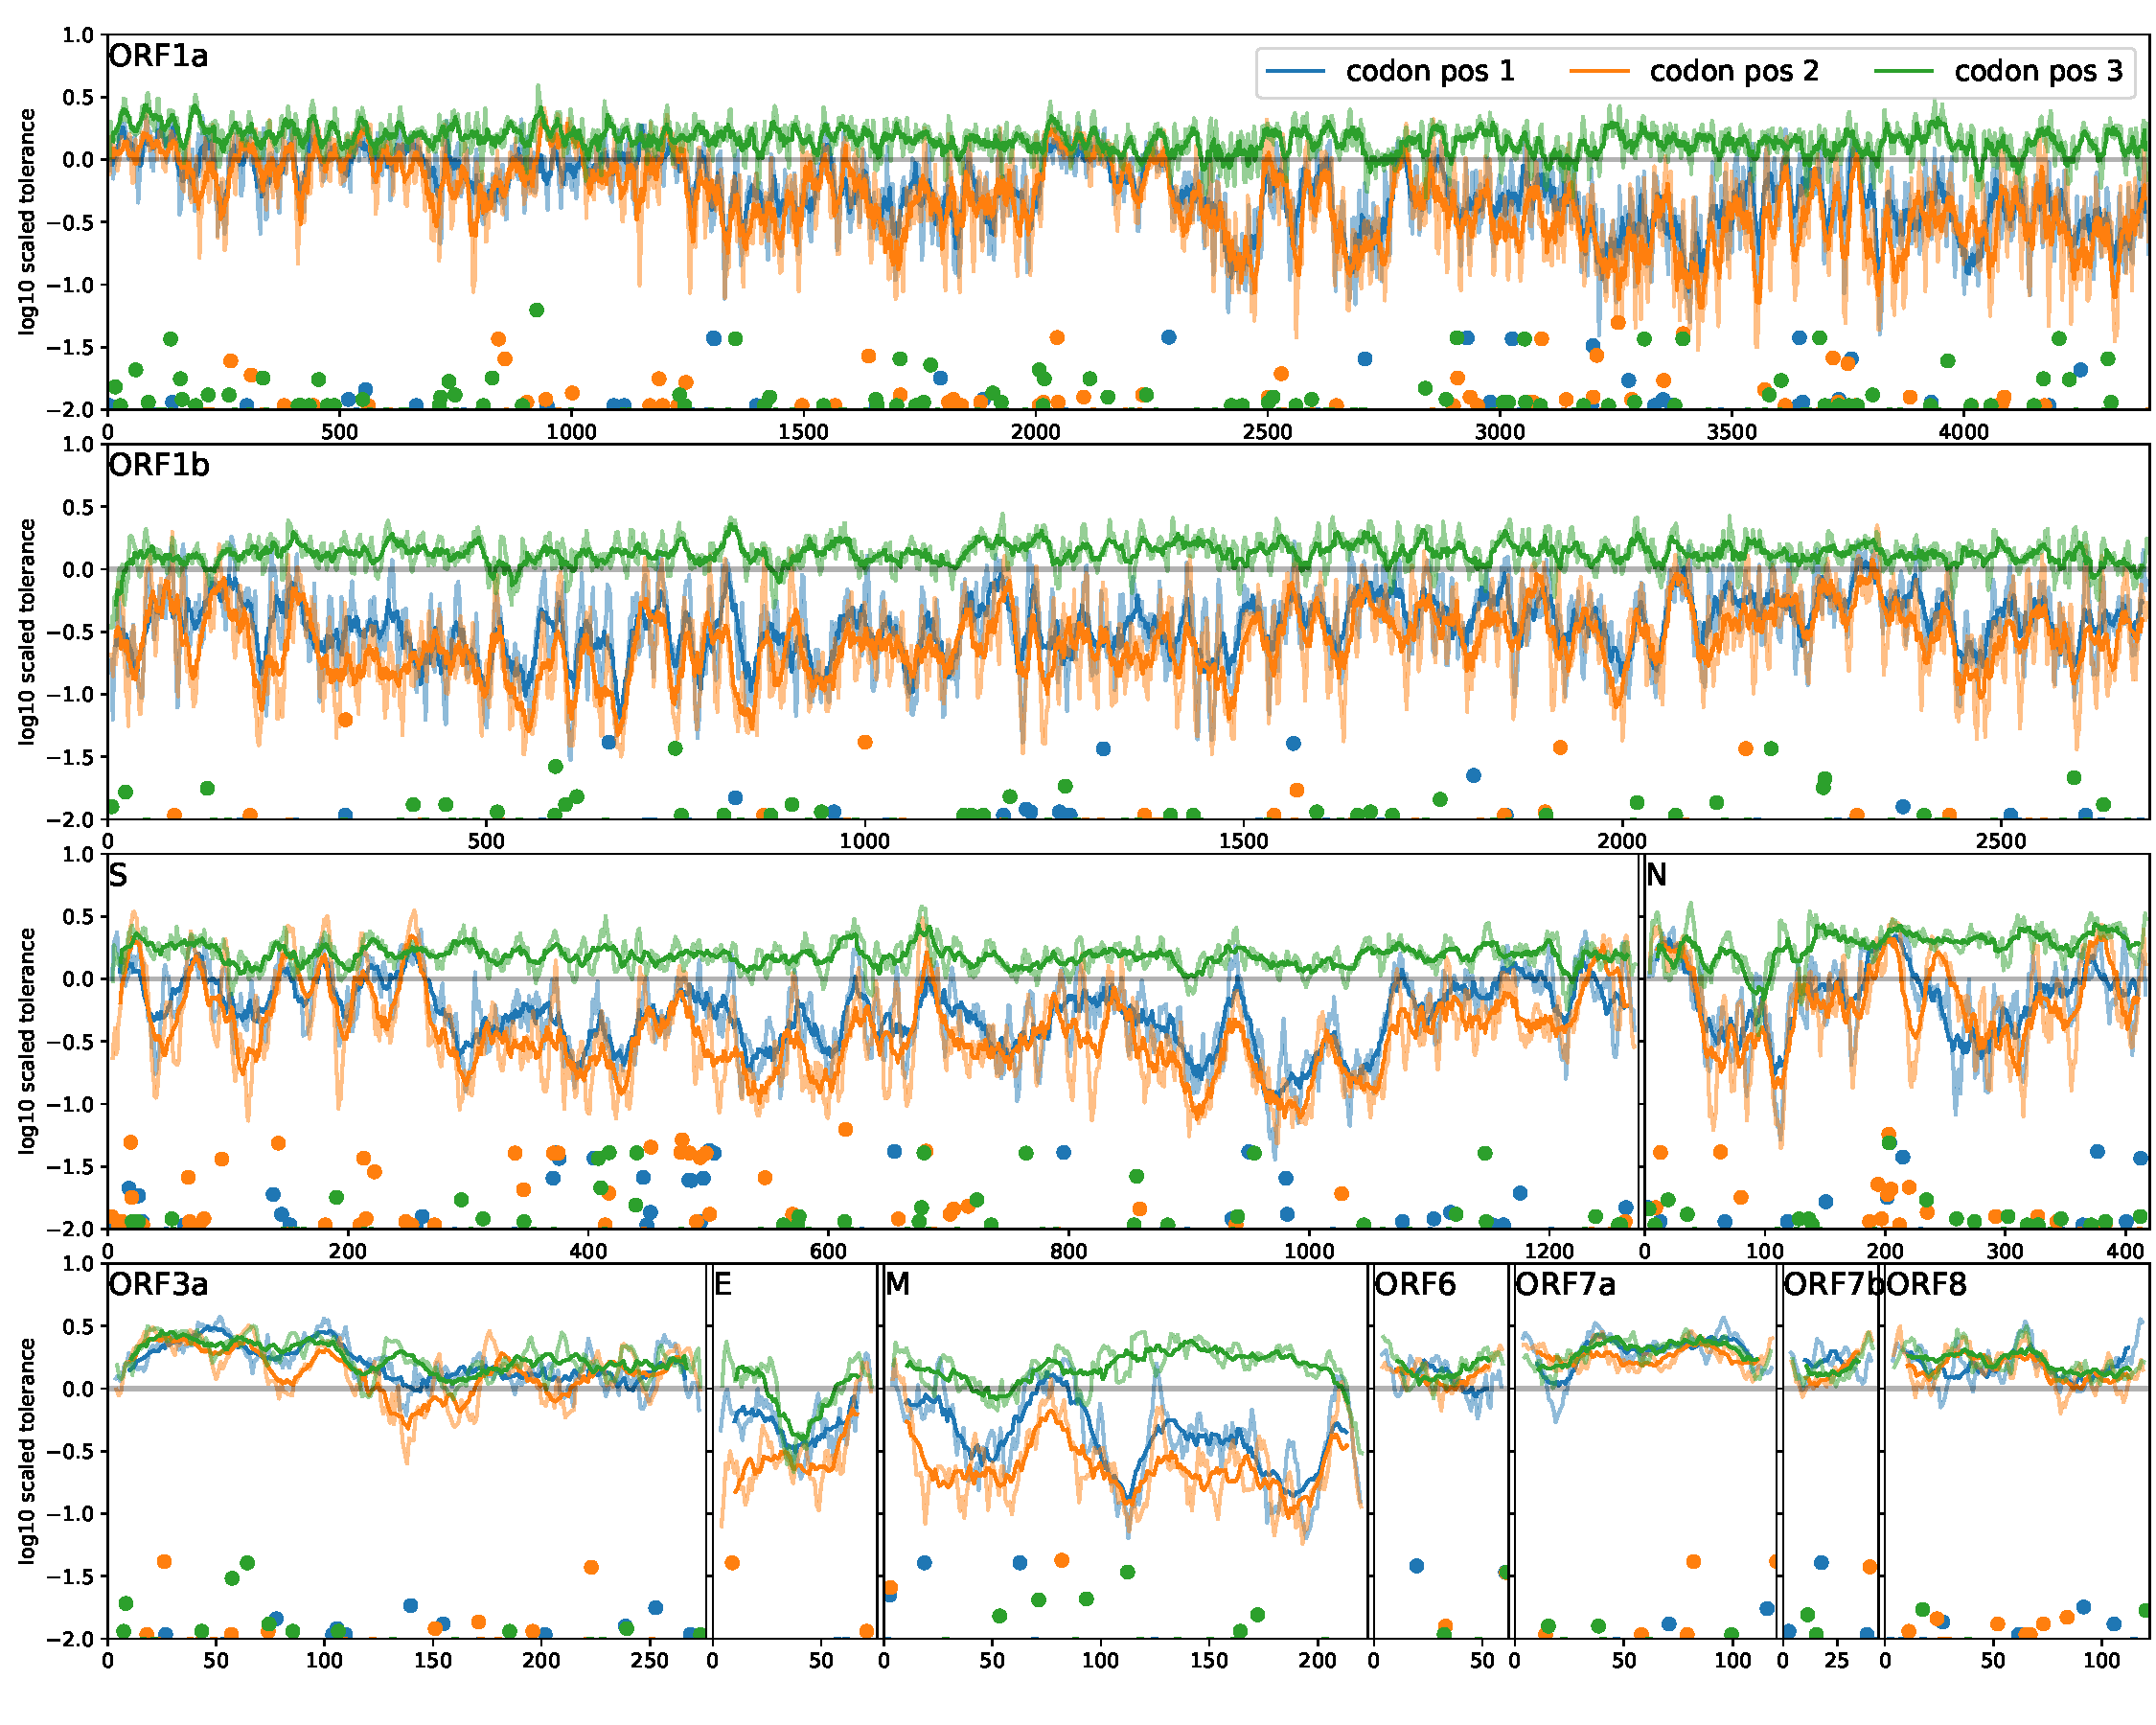
\includegraphics[width=\textwidth]{figures/fitness_landscape.pdf}
    \caption{{\bf Landscape of selective constraint along the SARS-CoV-2 genome.}
    Solid lines show sliding window smoothing of estimated mutational tolerance at 1st, 2nd, and 3rd positions for a window size of 20 and 7 (faint lines) sites.
    The markers below the lines are a qualitative indication of variable positions across SARS-CoV-2 diversity.
    \label{fig:fitness_landscape_supp}}
 \end{figure}

\onecolumngrid
\section*{Divergence summaries}

\begin{figure*}
    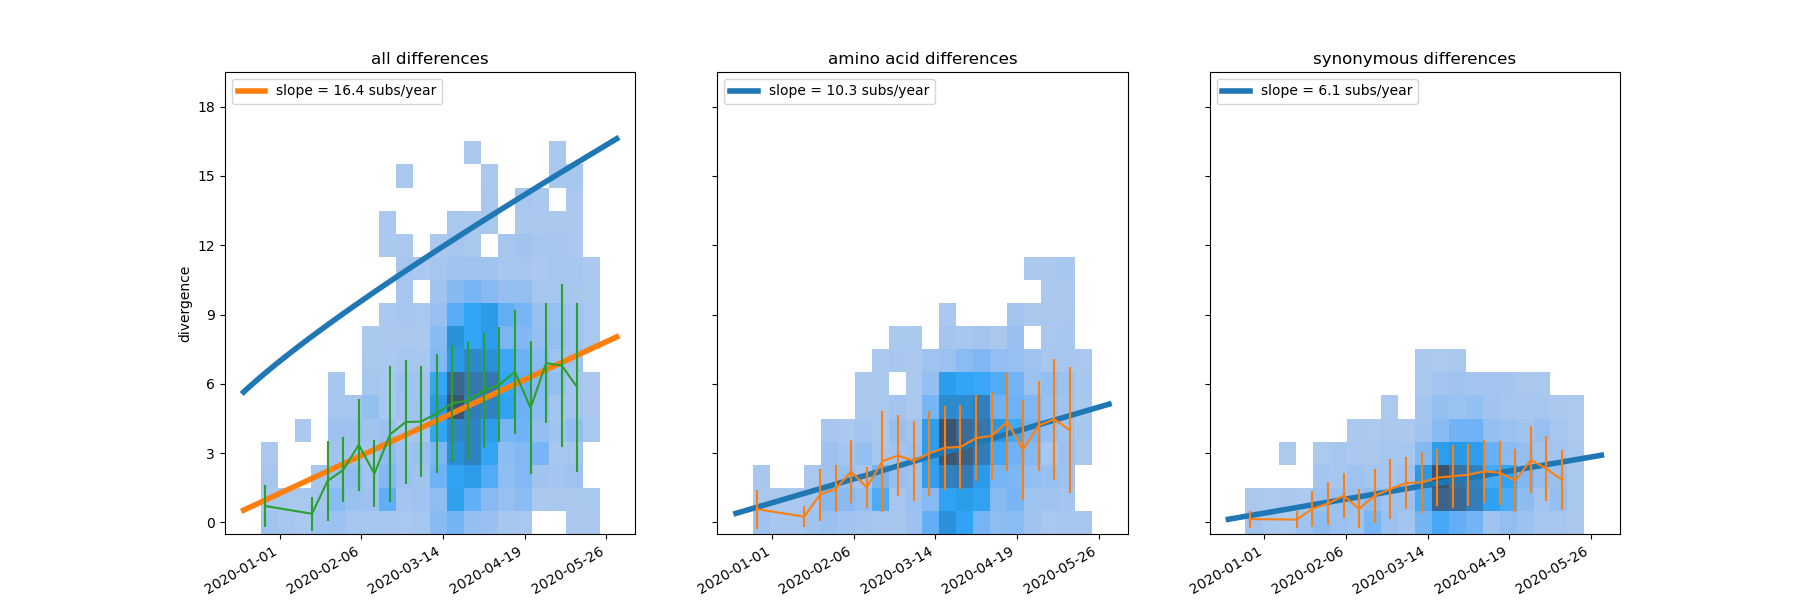
\includegraphics[width=\textwidth]{figures/rtt/19A_rtt.png}
    \caption{{\bf Divergence increases linearly with time in clade 19A.}
    \label{fig:19A_divergence}}
\end{figure*}

\begin{figure*}
    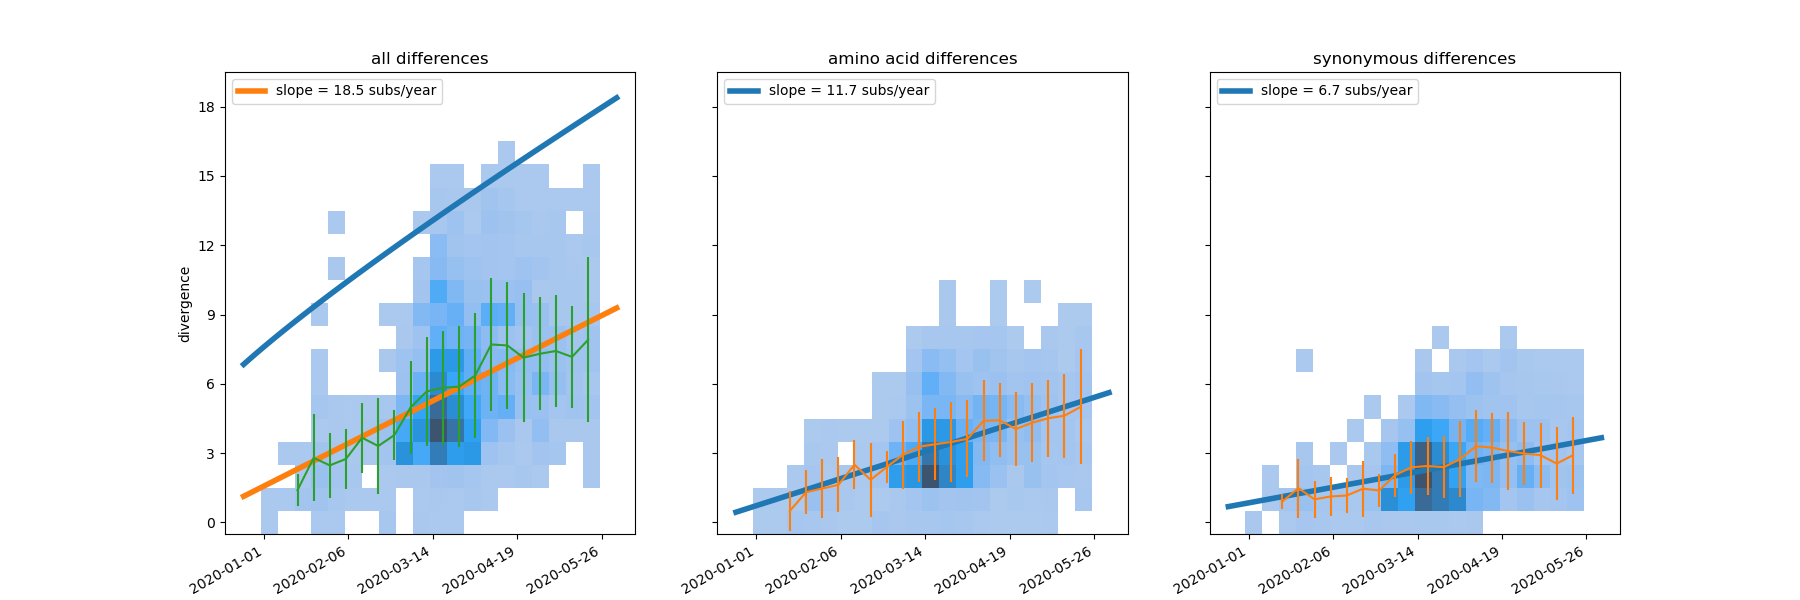
\includegraphics[width=\textwidth]{figures/rtt/19B_rtt.png}
    \caption{{\bf Divergence increases linearly with time in clade 19B.}
    \label{fig:19B_divergence}}
\end{figure*}

\begin{figure*}
    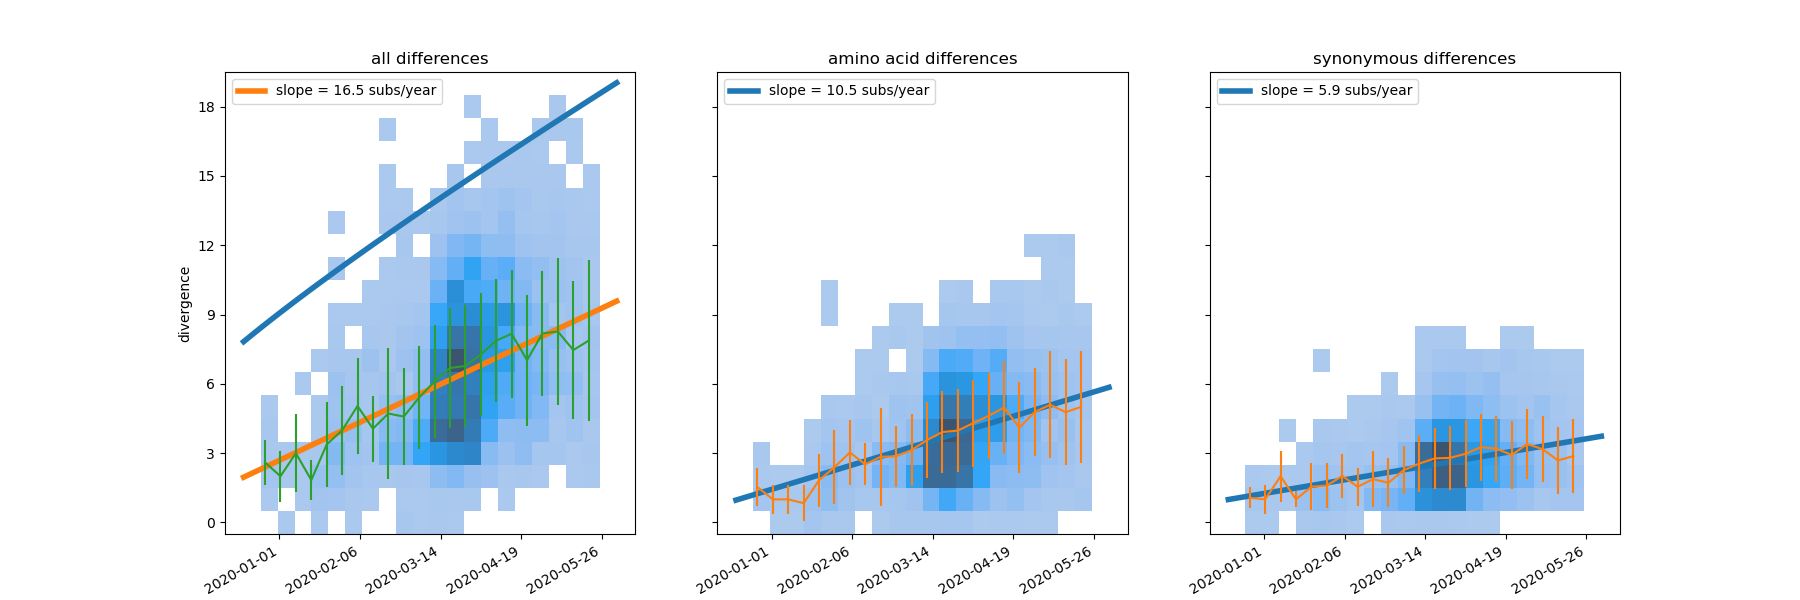
\includegraphics[width=\textwidth]{figures/rtt/19B+_rtt.png}
    \caption{{\bf Divergence increases linearly with time in clade 19B+.}
    This figure contains sequences in clades 19 A and B rooted on clade 19B.
    \label{fig:19B+_divergence}}
\end{figure*}

\begin{figure*}
    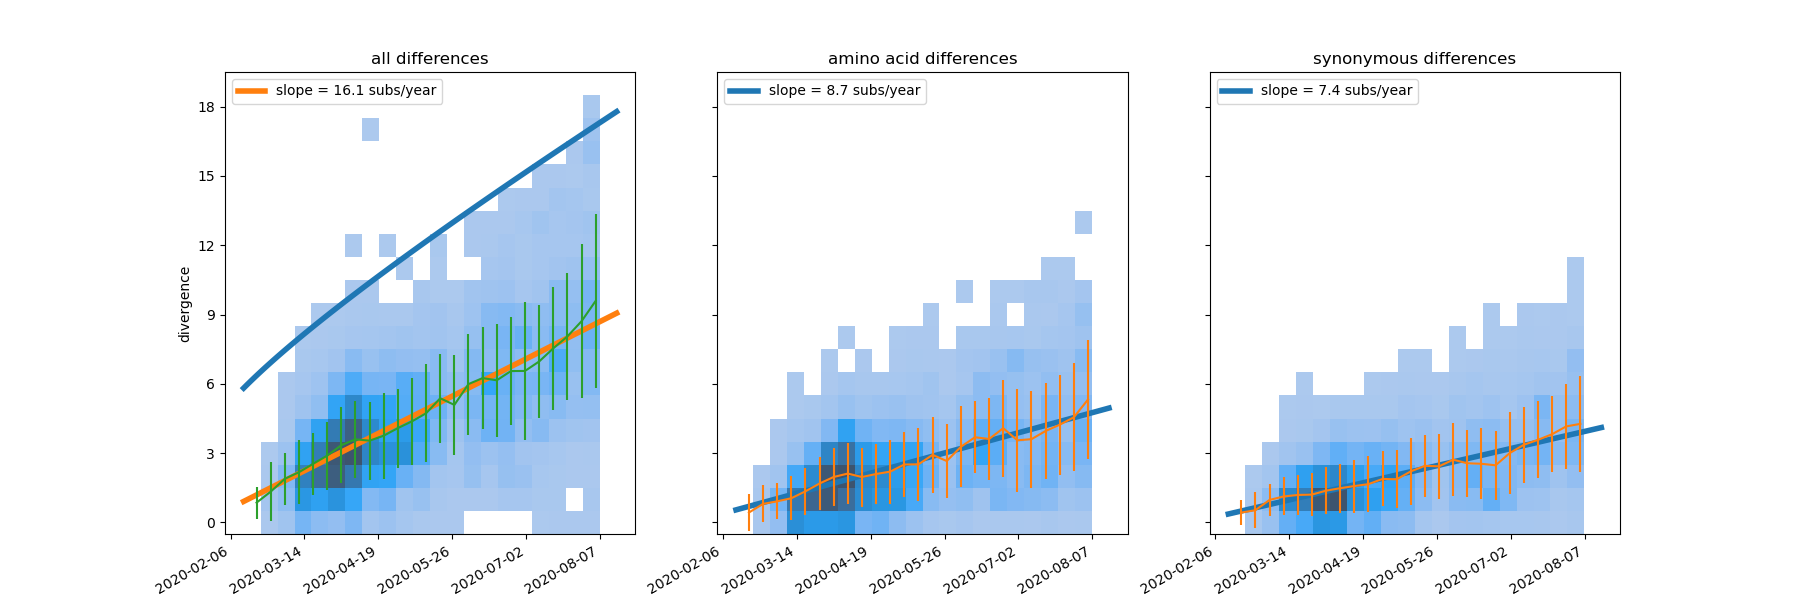
\includegraphics[width=\textwidth]{figures/rtt/20A_rtt.png}
    \caption{{\bf Divergence increases linearly with time in clade 20A.}
    \label{fig:20A_divergence}}
\end{figure*}

\begin{figure*}
    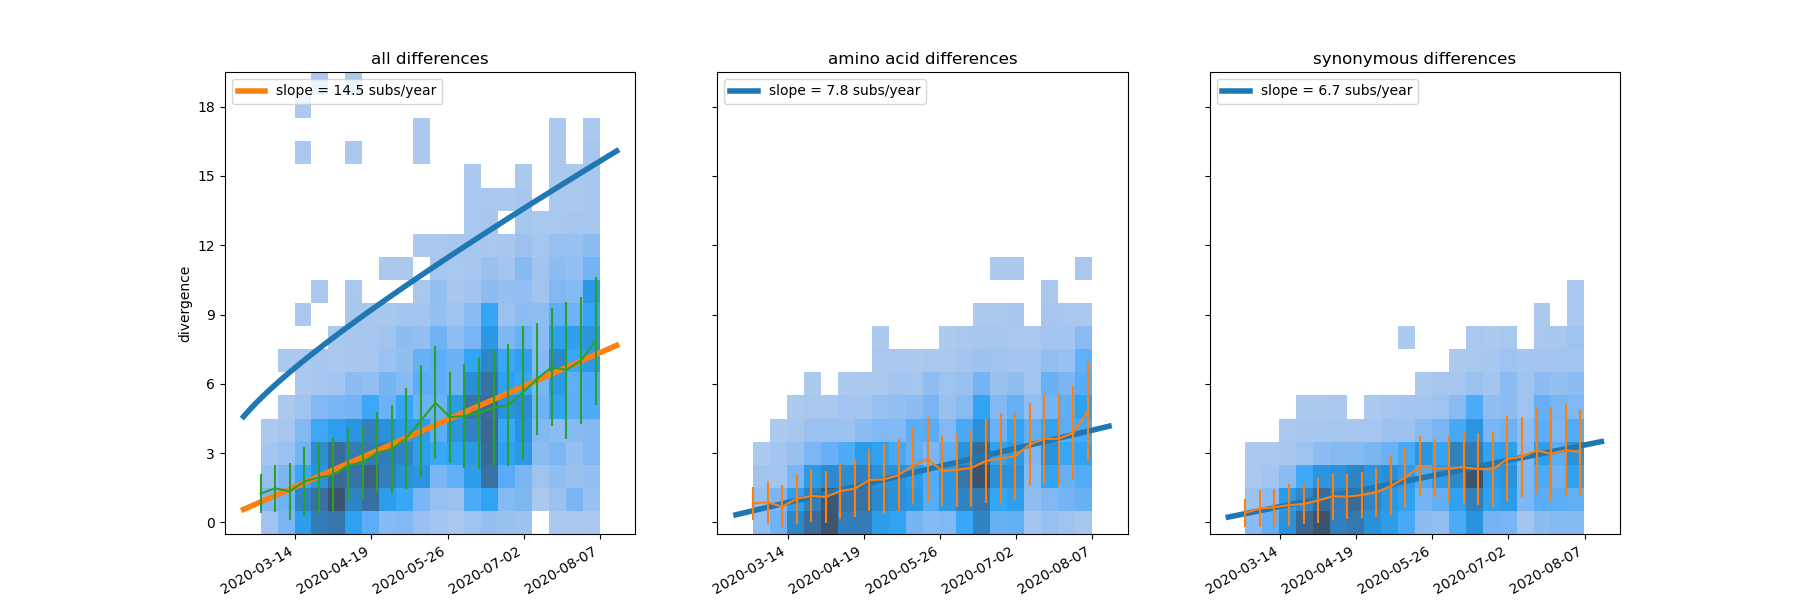
\includegraphics[width=\textwidth]{figures/rtt/20B_rtt.png}
    \caption{{\bf Divergence increases linearly with time in clade 20B.}
    \label{fig:20B_divergence}}
\end{figure*}

\begin{figure*}
    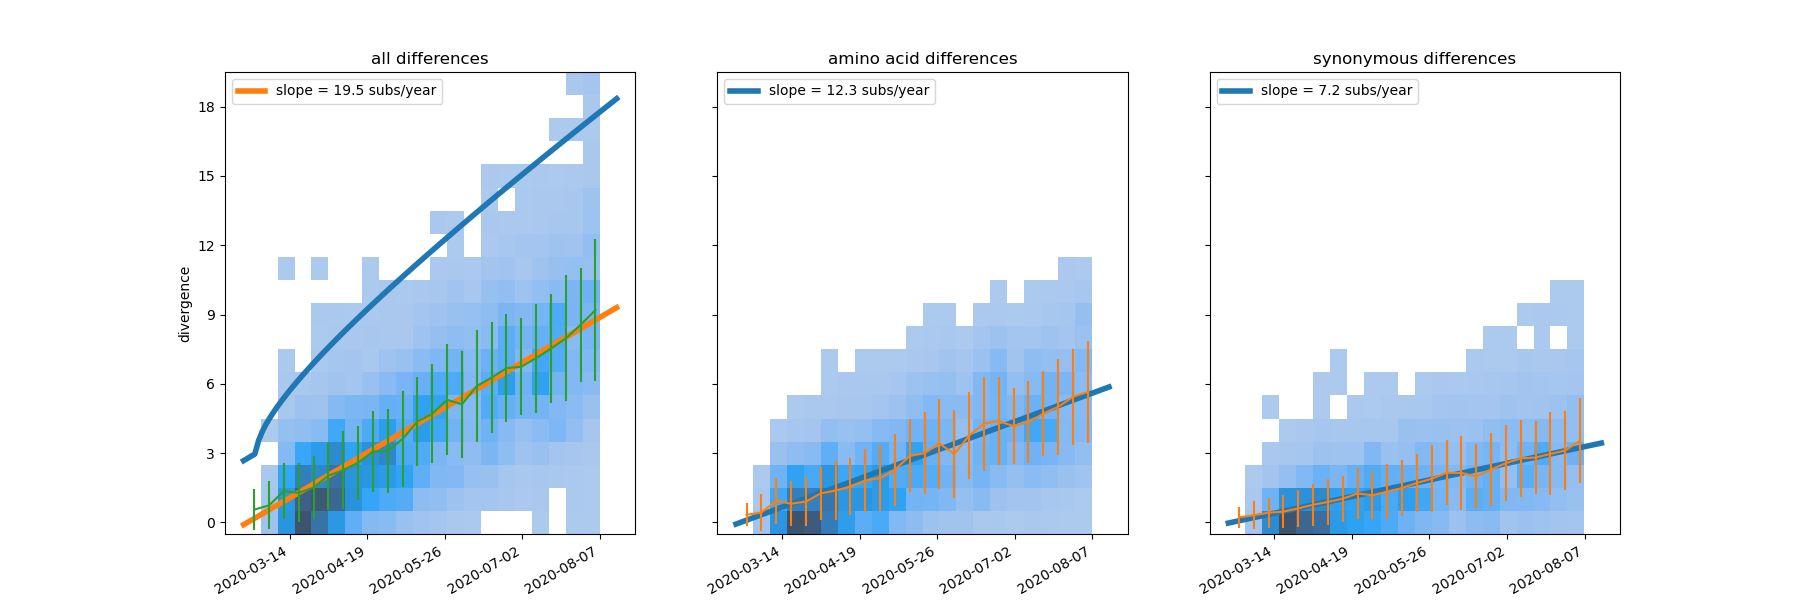
\includegraphics[width=\textwidth]{figures/rtt/20C_rtt.png}
    \caption{{\bf Divergence increases linearly with time in clade 20C.}
    \label{fig:20C_divergence}}
\end{figure*}


\begin{figure*}
    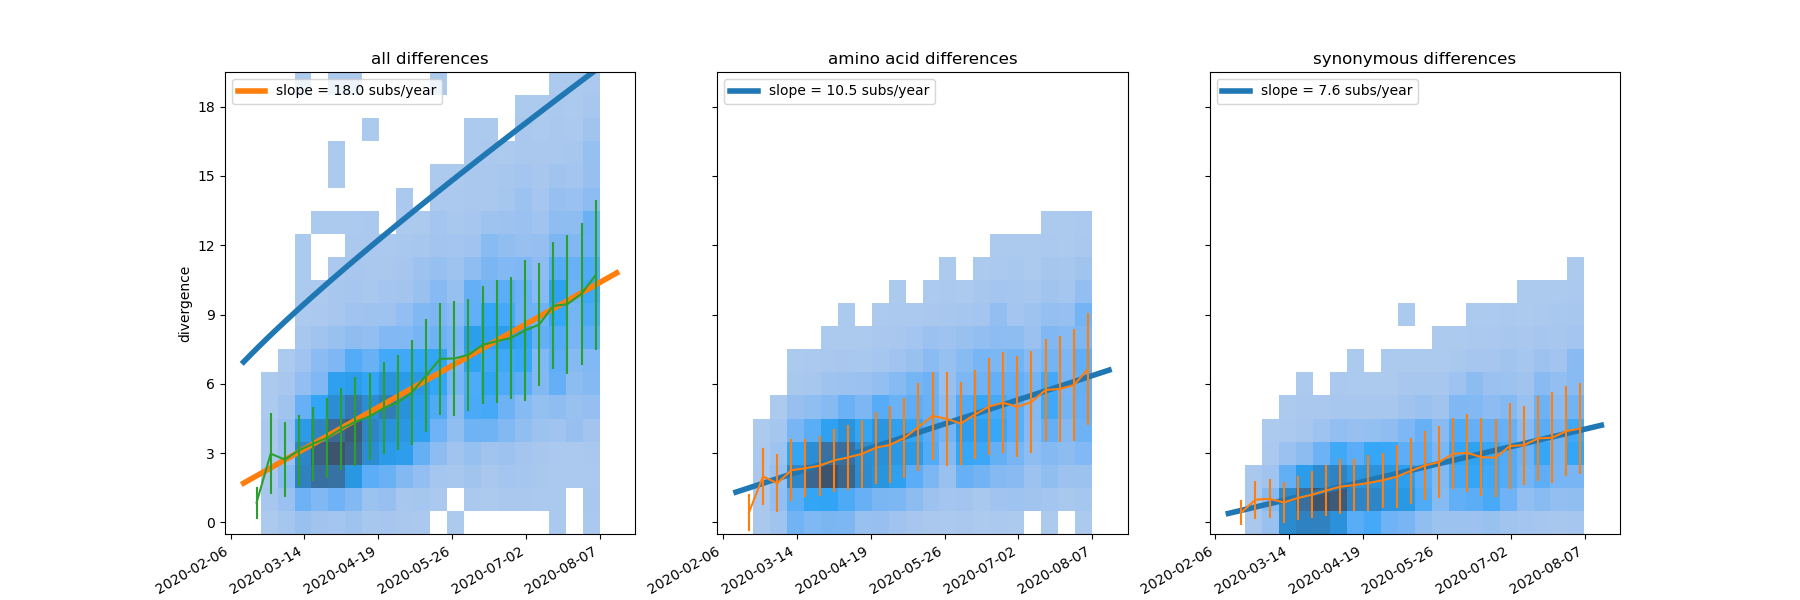
\includegraphics[width=\textwidth]{figures/rtt/20A+_rtt.png}
    \caption{{\bf Divergence increases linearly with time in clade 20A+.}
    This figure contains sequences in clades 20A,B,C,D rooted on clade 20A.
    \label{fig:20A+_divergence}}
\end{figure*}



\begin{figure*}
    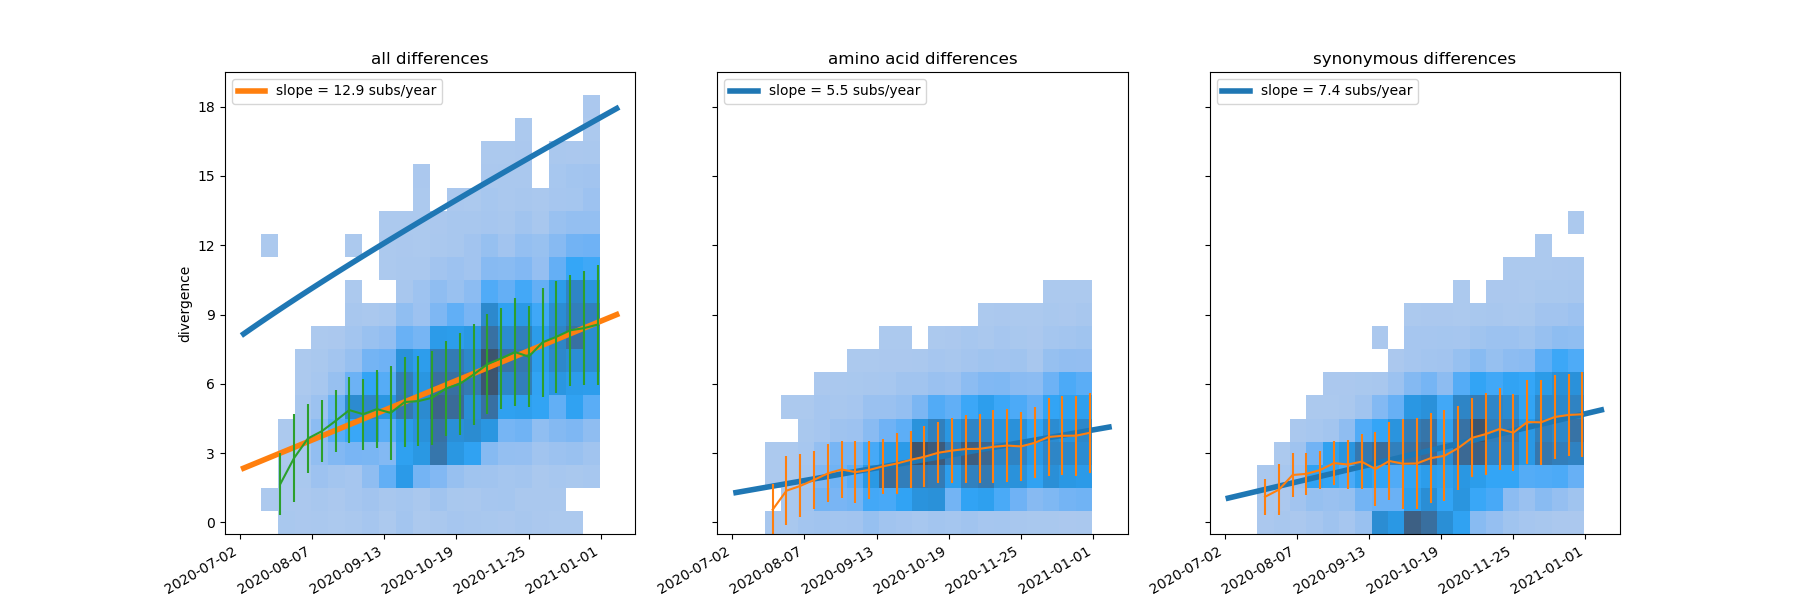
\includegraphics[width=\textwidth]{figures/rtt/20E_rtt.png}
    \caption{{\bf Divergence increases linearly with time in clade 20E.}
    \label{fig:20E_divergence}}
\end{figure*}

\begin{figure*}
    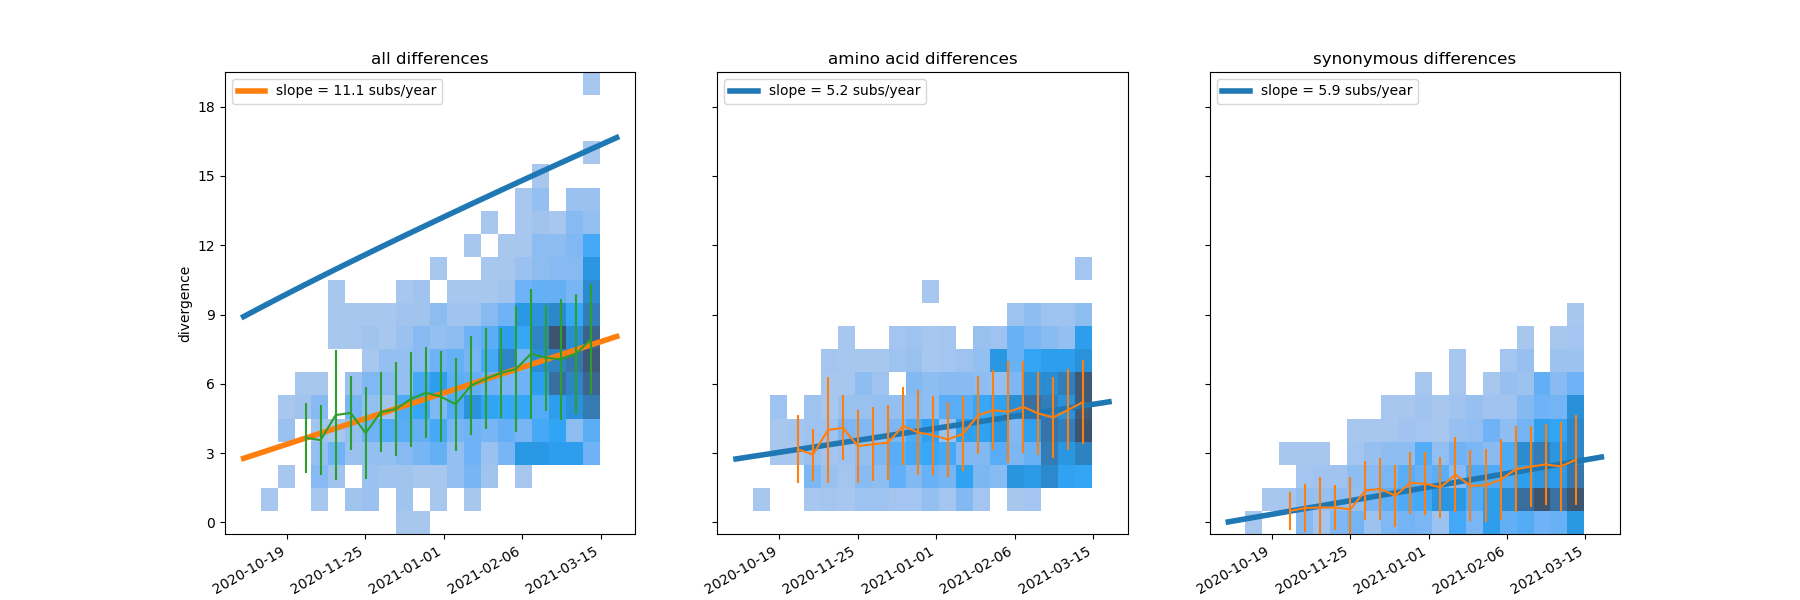
\includegraphics[width=\textwidth]{figures/rtt/20H_rtt.png}
    \caption{{\bf Divergence increases linearly with time in clade 20H (Beta).}
    \label{fig:20H_divergence}}
\end{figure*}

\begin{figure*}
    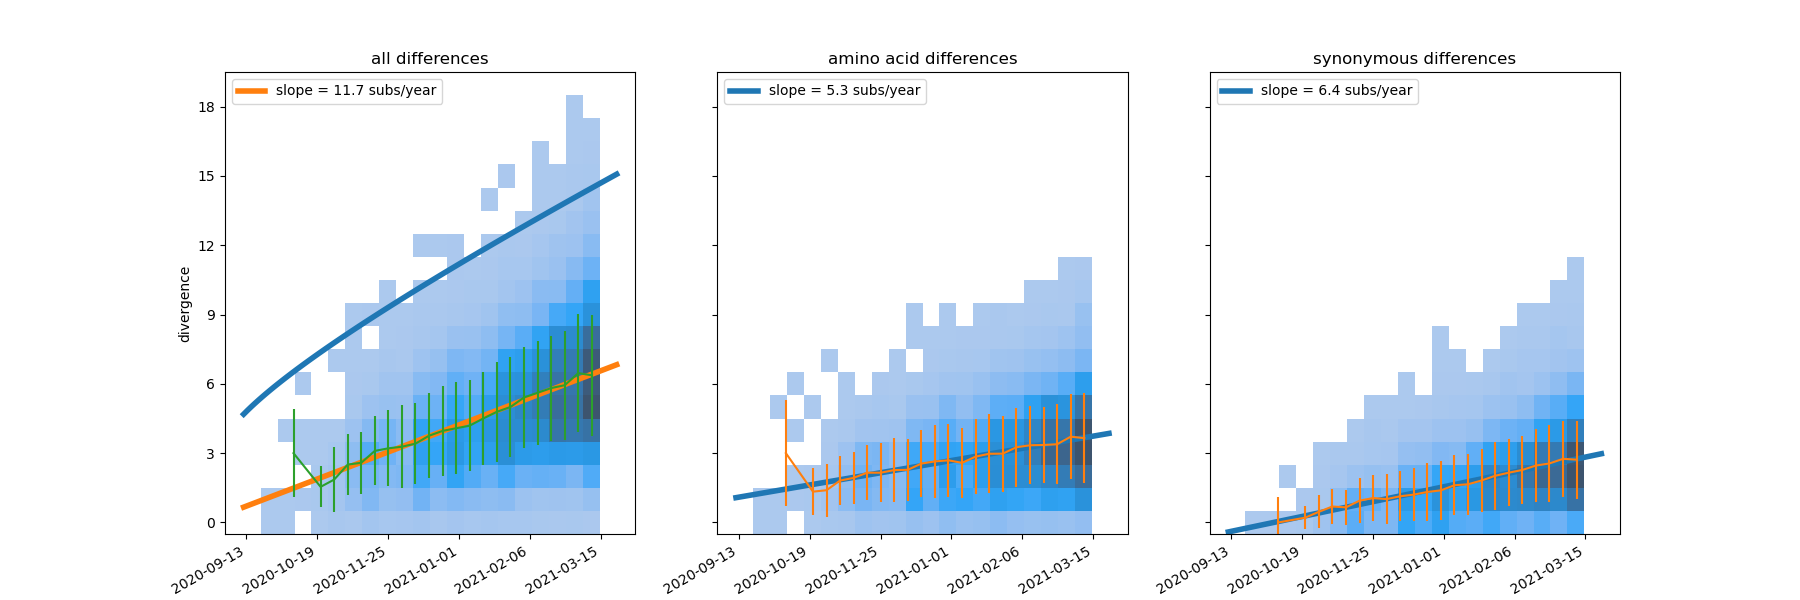
\includegraphics[width=\textwidth]{figures/rtt/20I_rtt.png}
    \caption{{\bf Divergence increases linearly with time in clade 20I (Alpha).}
    \label{fig:20I_divergence}}
\end{figure*}

\begin{figure*}
    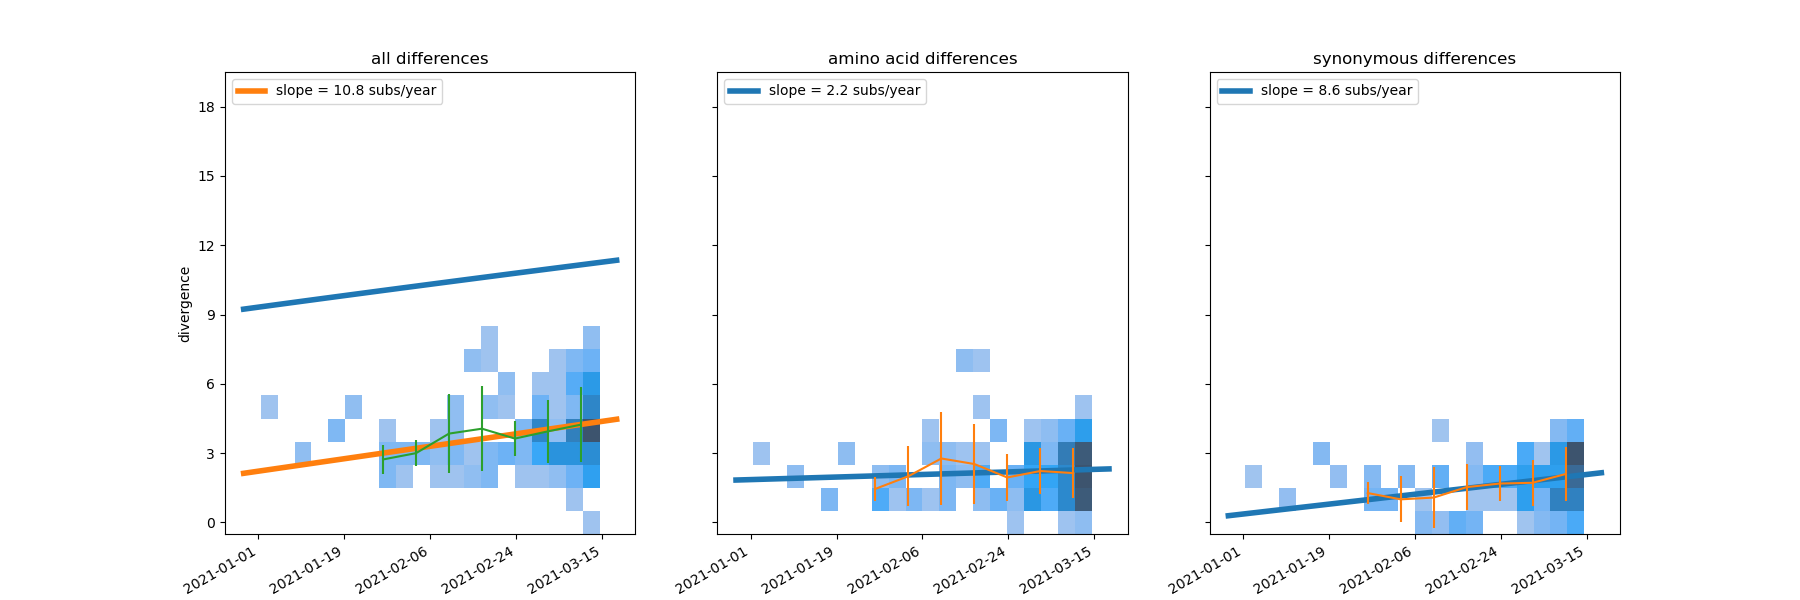
\includegraphics[width=\textwidth]{figures/rtt/20J_rtt.png}
    \caption{{\bf Divergence increases linearly with time in clade 20J (Gamma).}
    \label{fig:20J_divergence}}
\end{figure*}


\begin{figure*}
    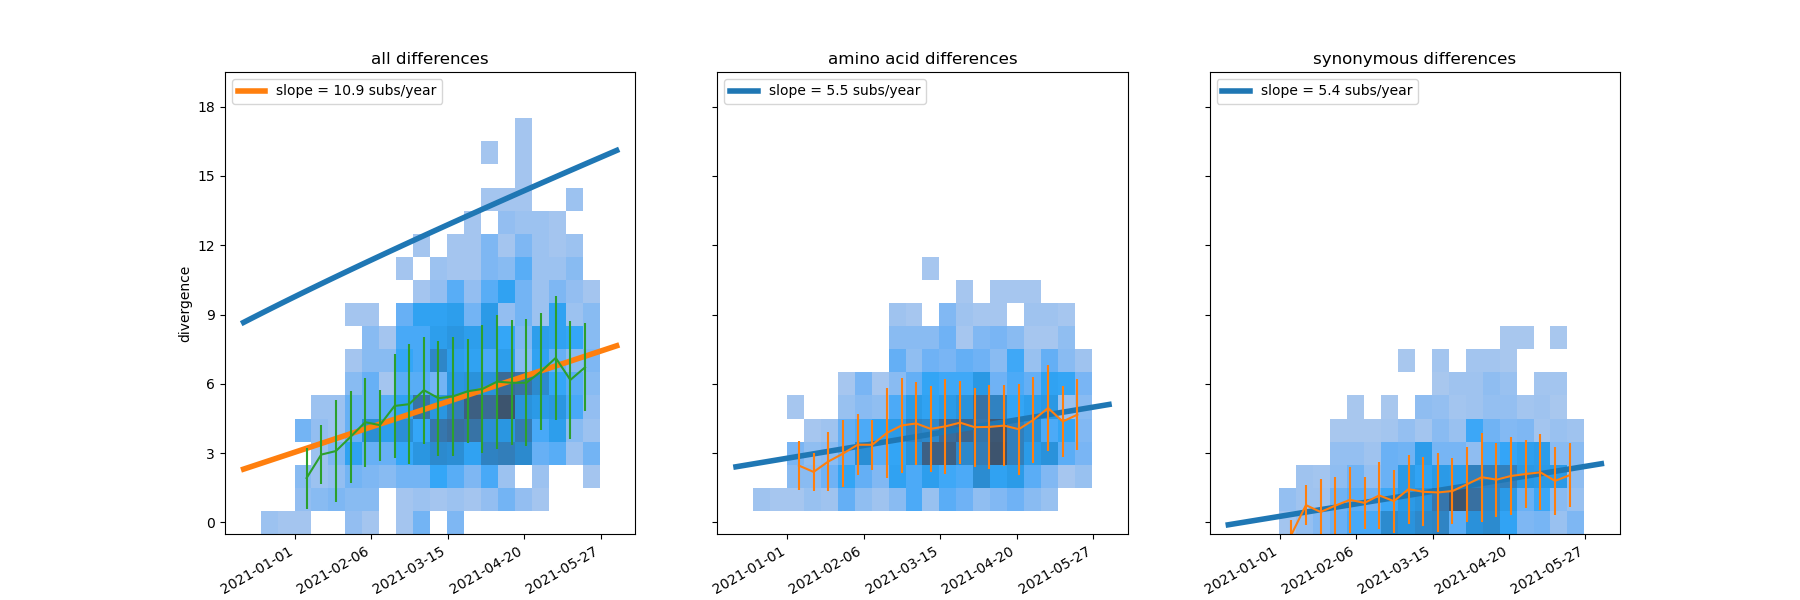
\includegraphics[width=\textwidth]{figures/rtt/21D_rtt.png}
    \caption{{\bf Divergence increases linearly with time in clade 21D (Eta).}
    \label{fig:21D_divergence}}
\end{figure*}

\begin{figure*}
    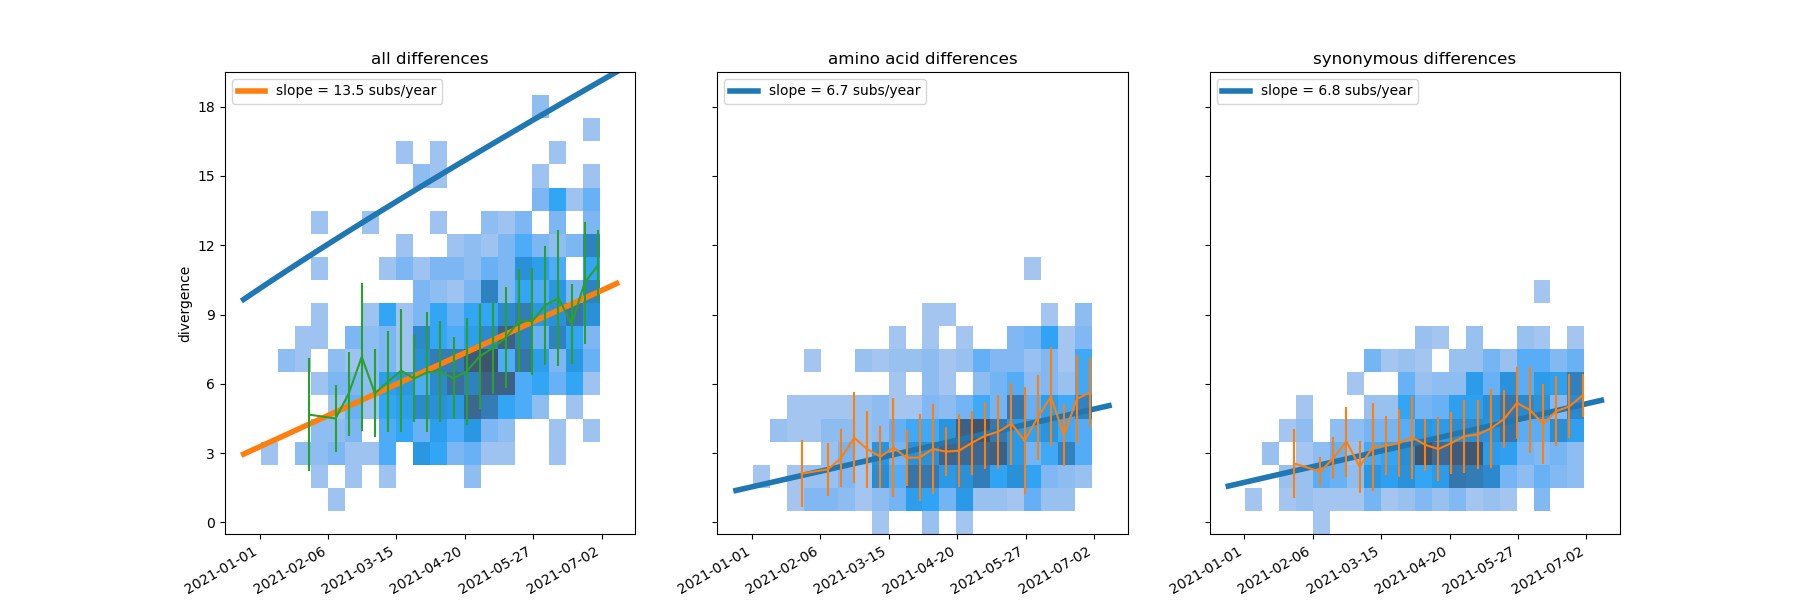
\includegraphics[width=\textwidth]{figures/rtt/21G_rtt.png}
    \caption{{\bf Divergence increases linearly with time in clade 21G (Lambda).}
    \label{fig:21G_divergence}}
\end{figure*}

\begin{figure*}
    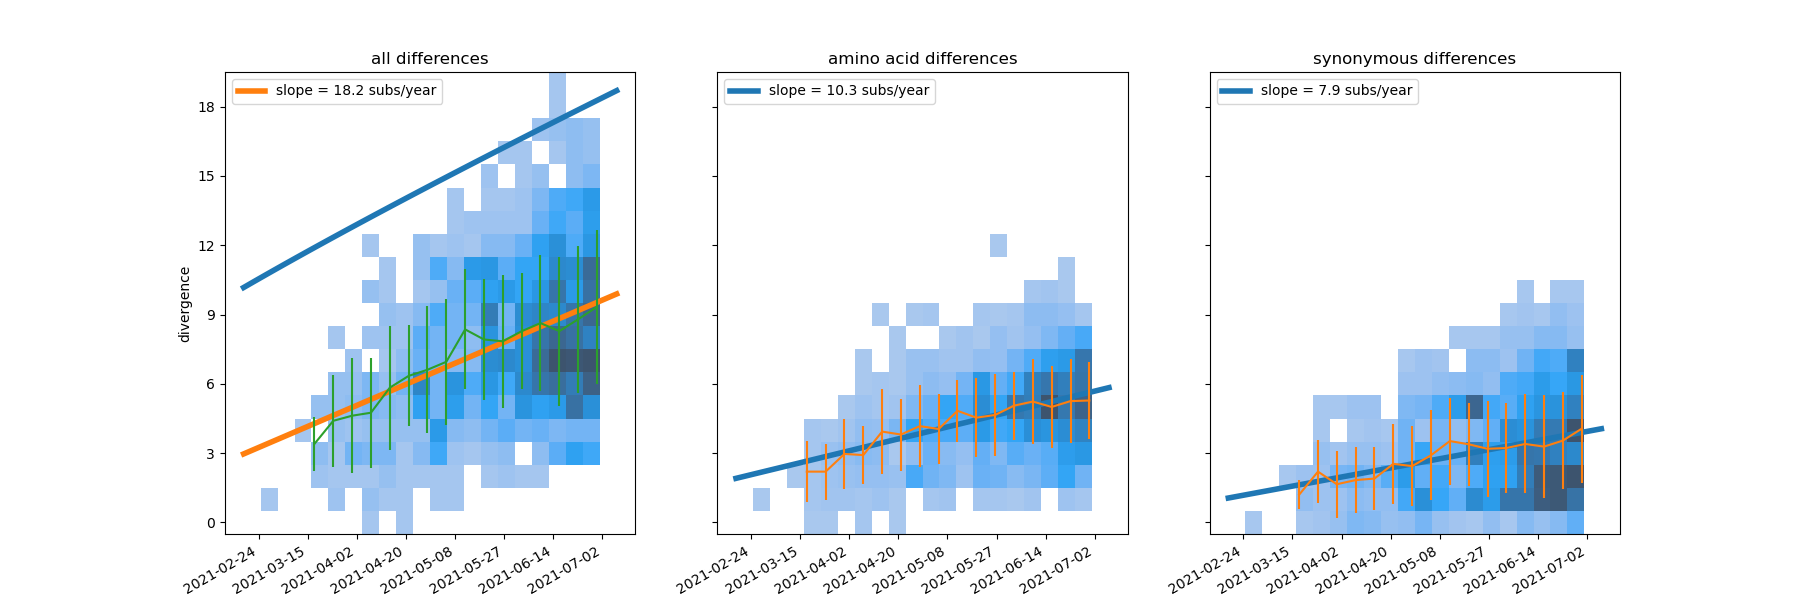
\includegraphics[width=\textwidth]{figures/rtt/21H_rtt.png}
    \caption{{\bf Divergence increases linearly with time in clade 21H (Mu).}
    \label{fig:21H_divergence}}
\end{figure*}

\begin{figure*}
    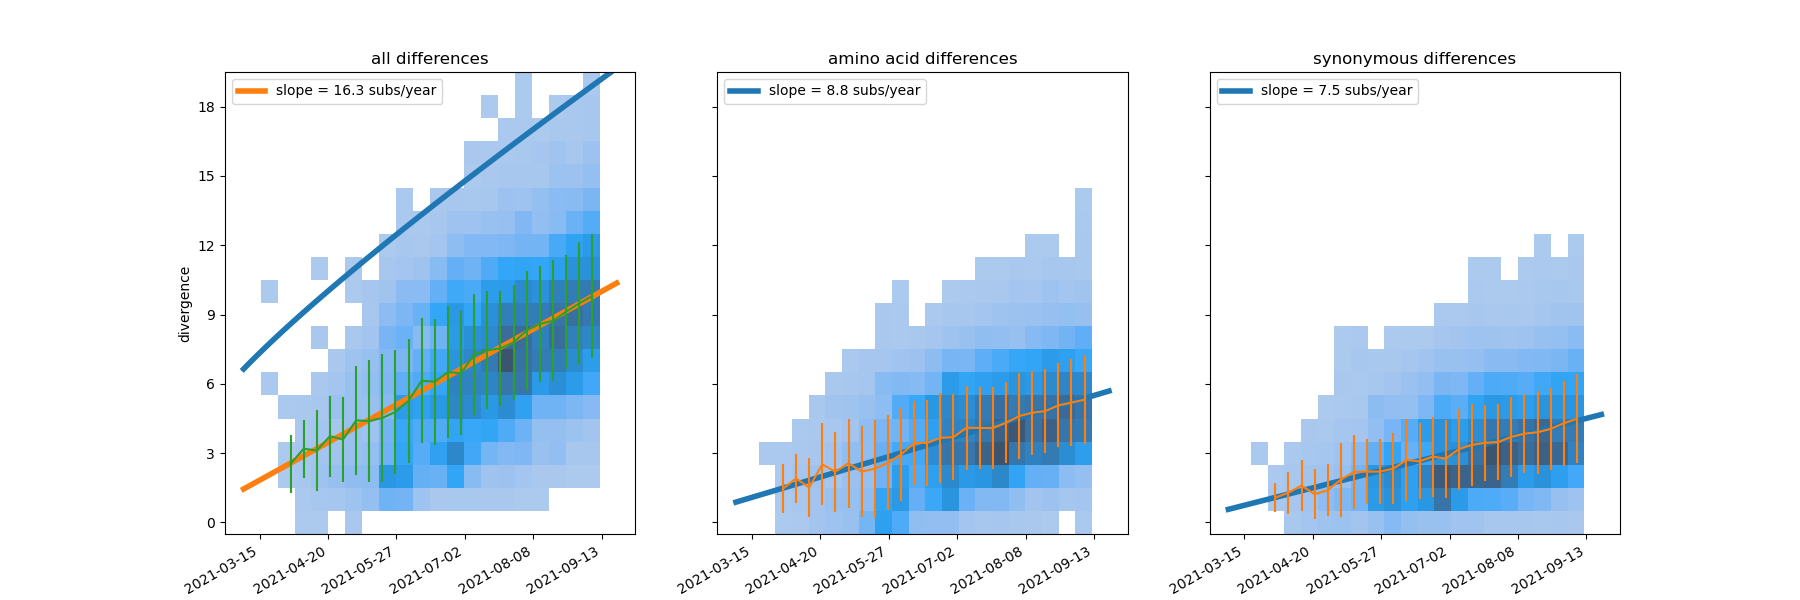
\includegraphics[width=\textwidth]{figures/rtt/21I_rtt.png}
    \caption{{\bf Divergence increases linearly with time in clade 21I (Delta).}
    \label{fig:21I_divergence}}
\end{figure*}

\begin{figure*}
    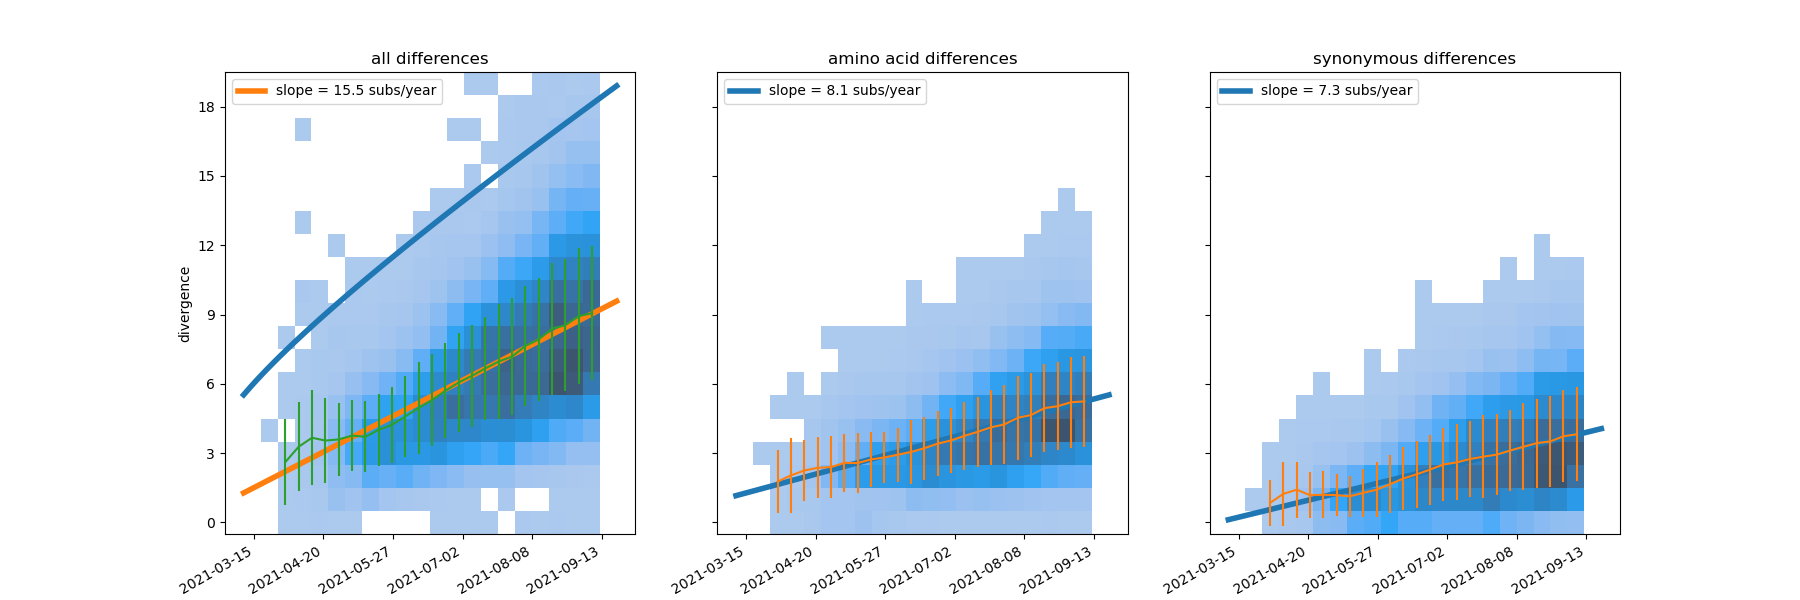
\includegraphics[width=\textwidth]{figures/rtt/21J_rtt.png}
    \caption{{\bf Divergence increases linearly with time in clade 21J (Delta).}
    \label{fig:21J_divergence}}
\end{figure*}

\begin{figure*}
    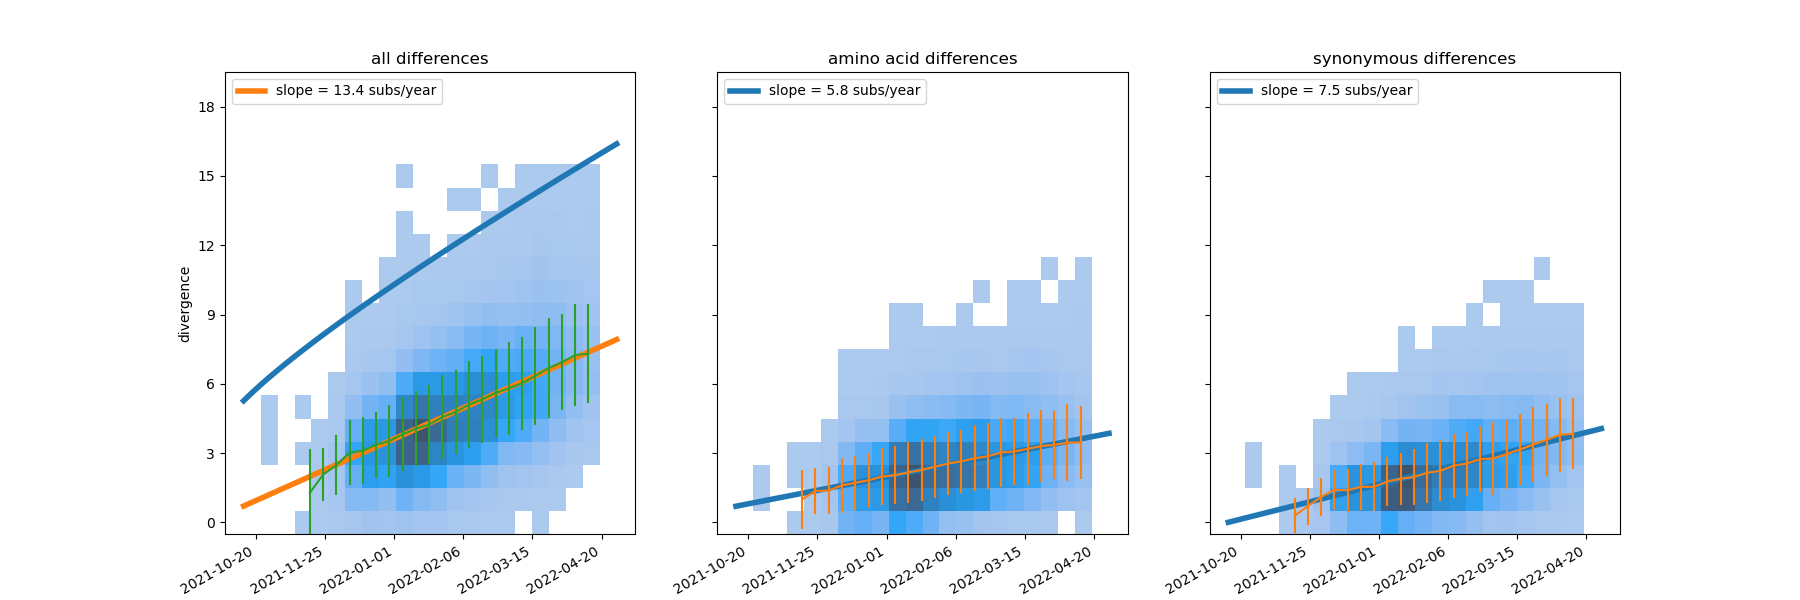
\includegraphics[width=\textwidth]{figures/rtt/21K_rtt.png}
    \caption{{\bf Divergence increases linearly with time in clade 21K (Omicron).}
    \label{fig:21K_divergence}}
\end{figure*}

\begin{figure*}
    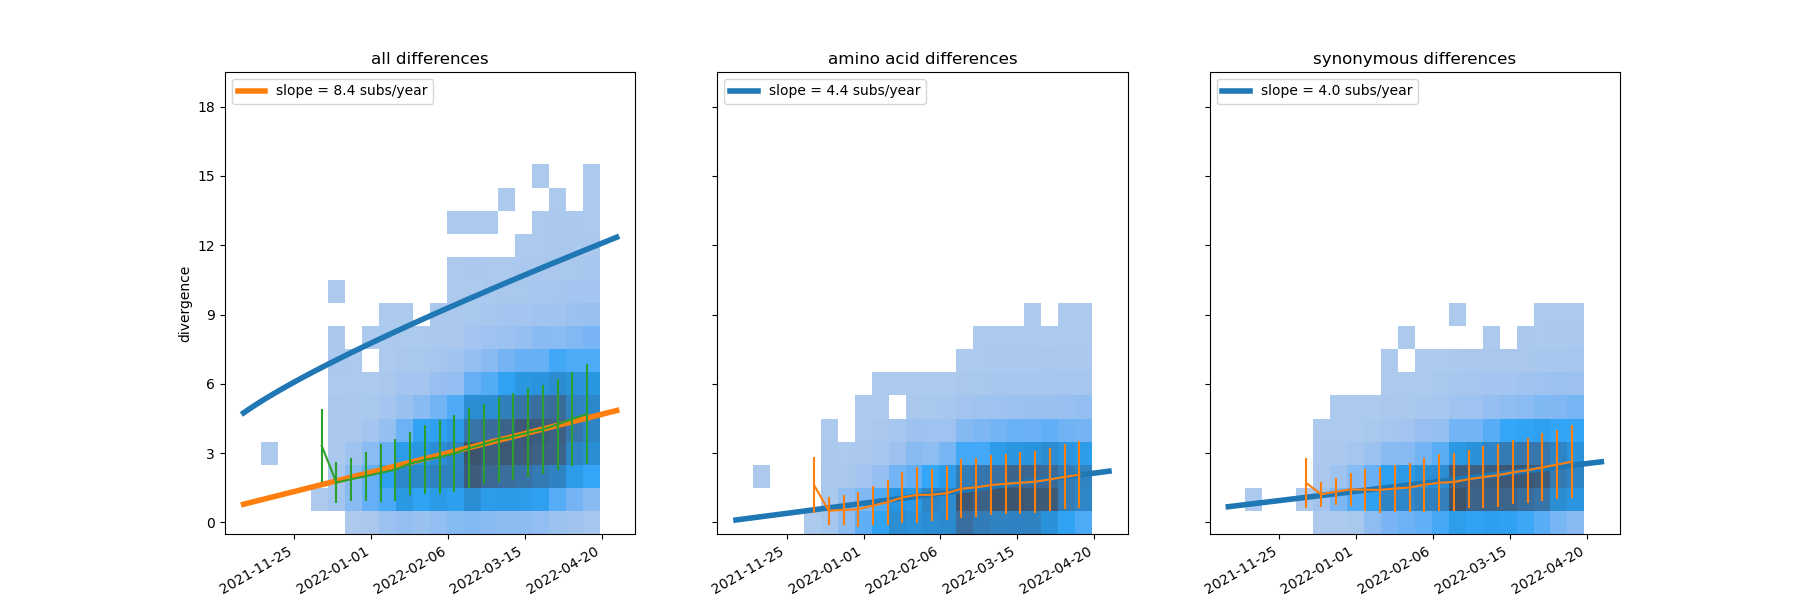
\includegraphics[width=\textwidth]{figures/rtt/21L_rtt.png}
    \caption{{\bf Divergence increases linearly with time in clade 21L (Omicron).}
    \label{fig:21L_divergence}}
\end{figure*}

\begin{figure*}
    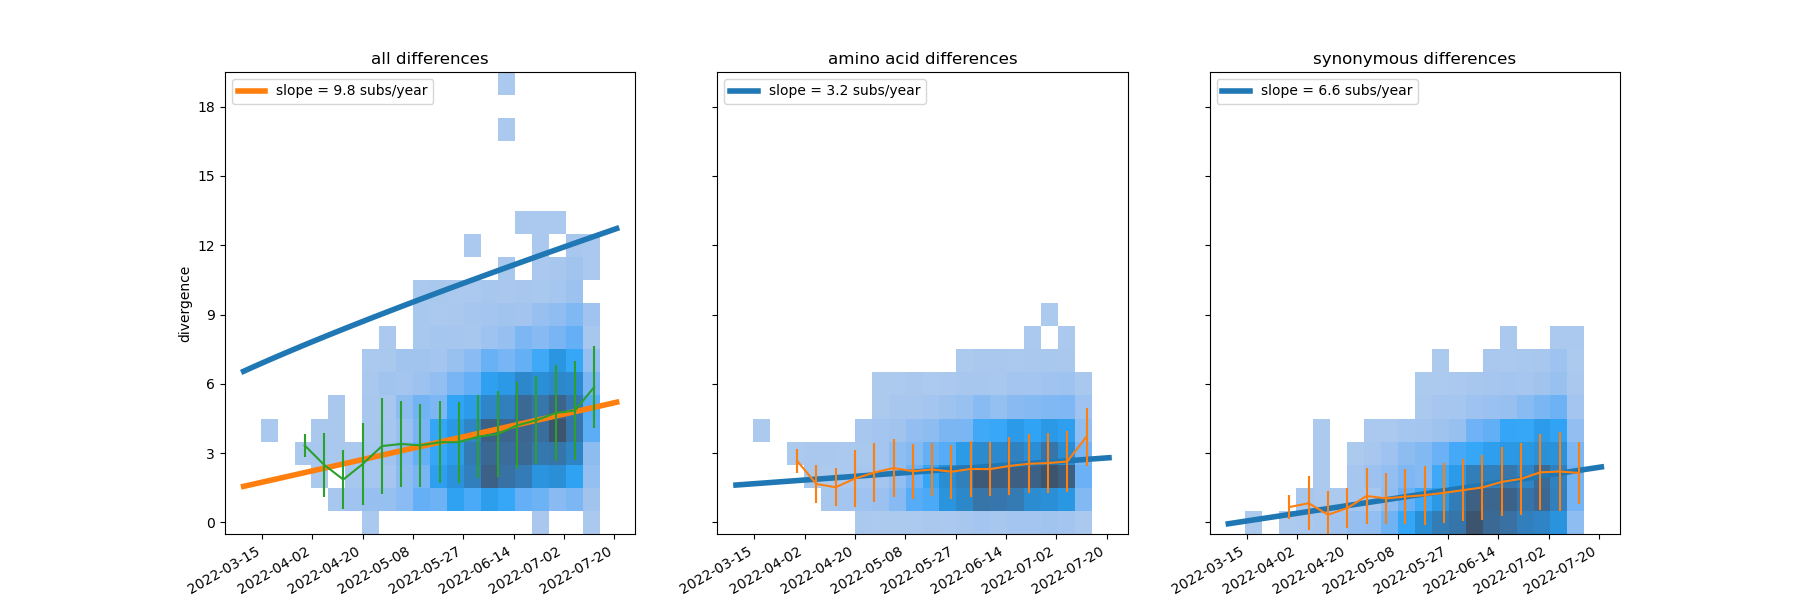
\includegraphics[width=\textwidth]{figures/rtt/22A_rtt.png}
    \caption{{\bf Divergence increases linearly with time in clade 22A (Omicron).}
    \label{fig:22A_divergence}}
\end{figure*}

\begin{figure*}
    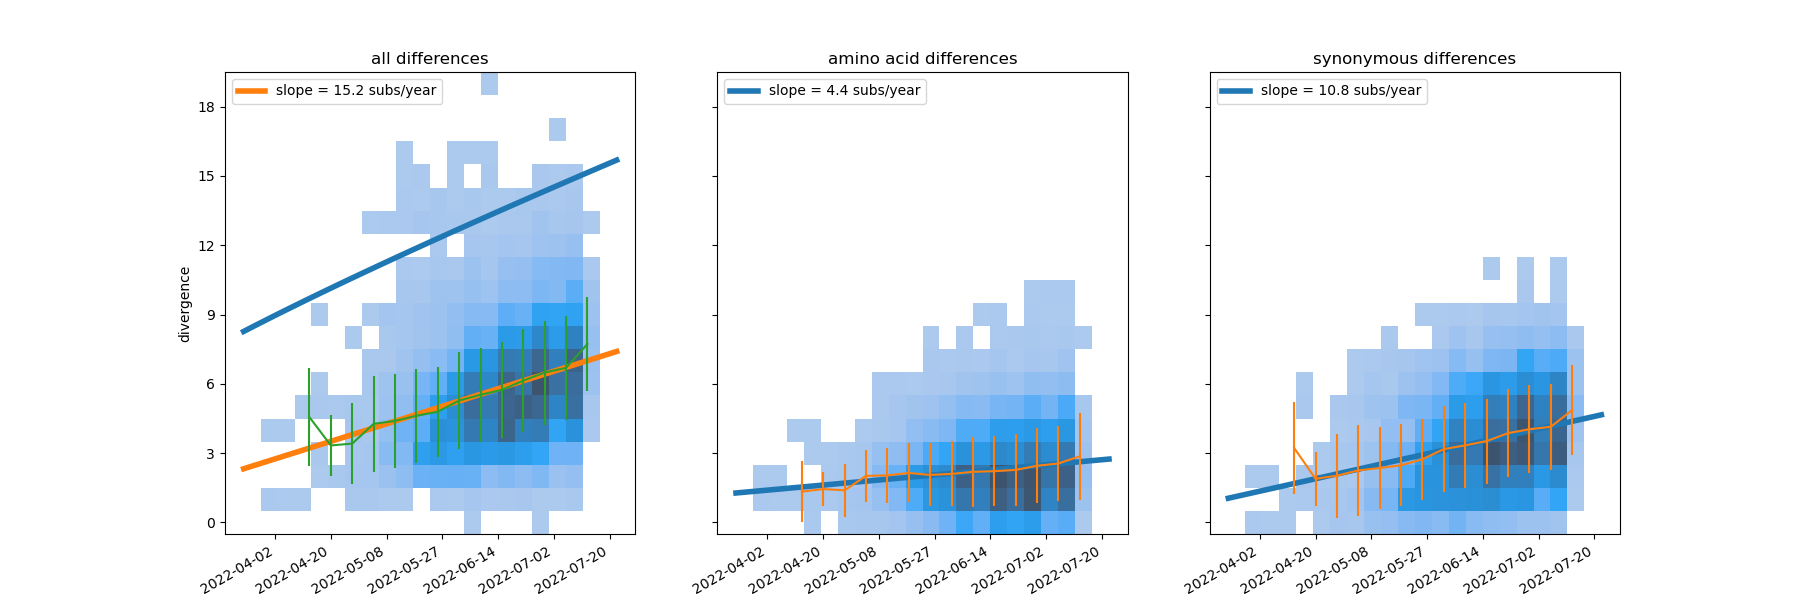
\includegraphics[width=\textwidth]{figures/rtt/22B_rtt.png}
    \caption{{\bf Divergence increases linearly with time in clade 22B (Omicron).}
    \label{fig:22B_divergence}}
\end{figure*}

% \section*{Mutation and haplotype summary}

\begin{figure*}[h]
    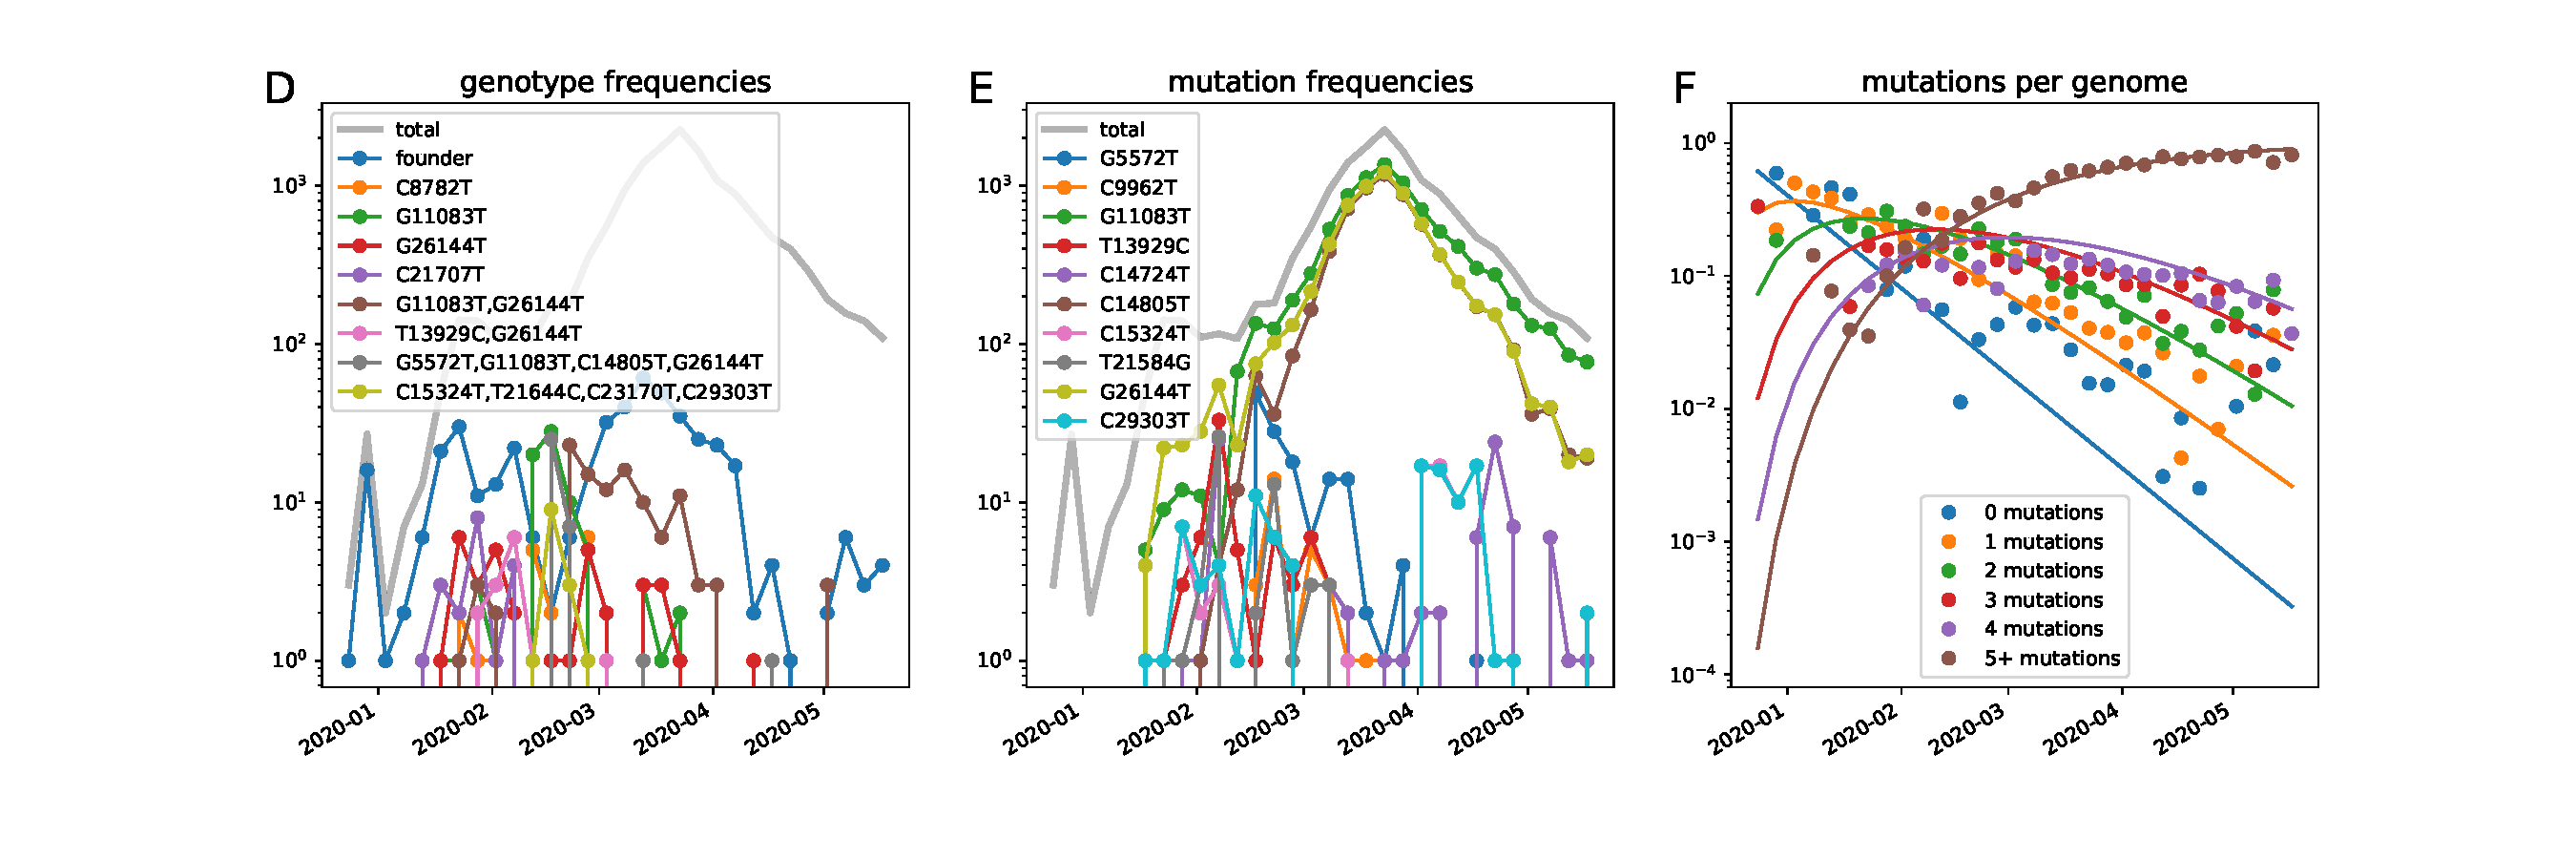
\includegraphics[width=\textwidth]{figures/counts/19A_counts.pdf}
    \caption{{\bf Diversification within clade 19A.}
    \label{fig:19A_counts}}
\end{figure*}

\begin{figure*}[h]
    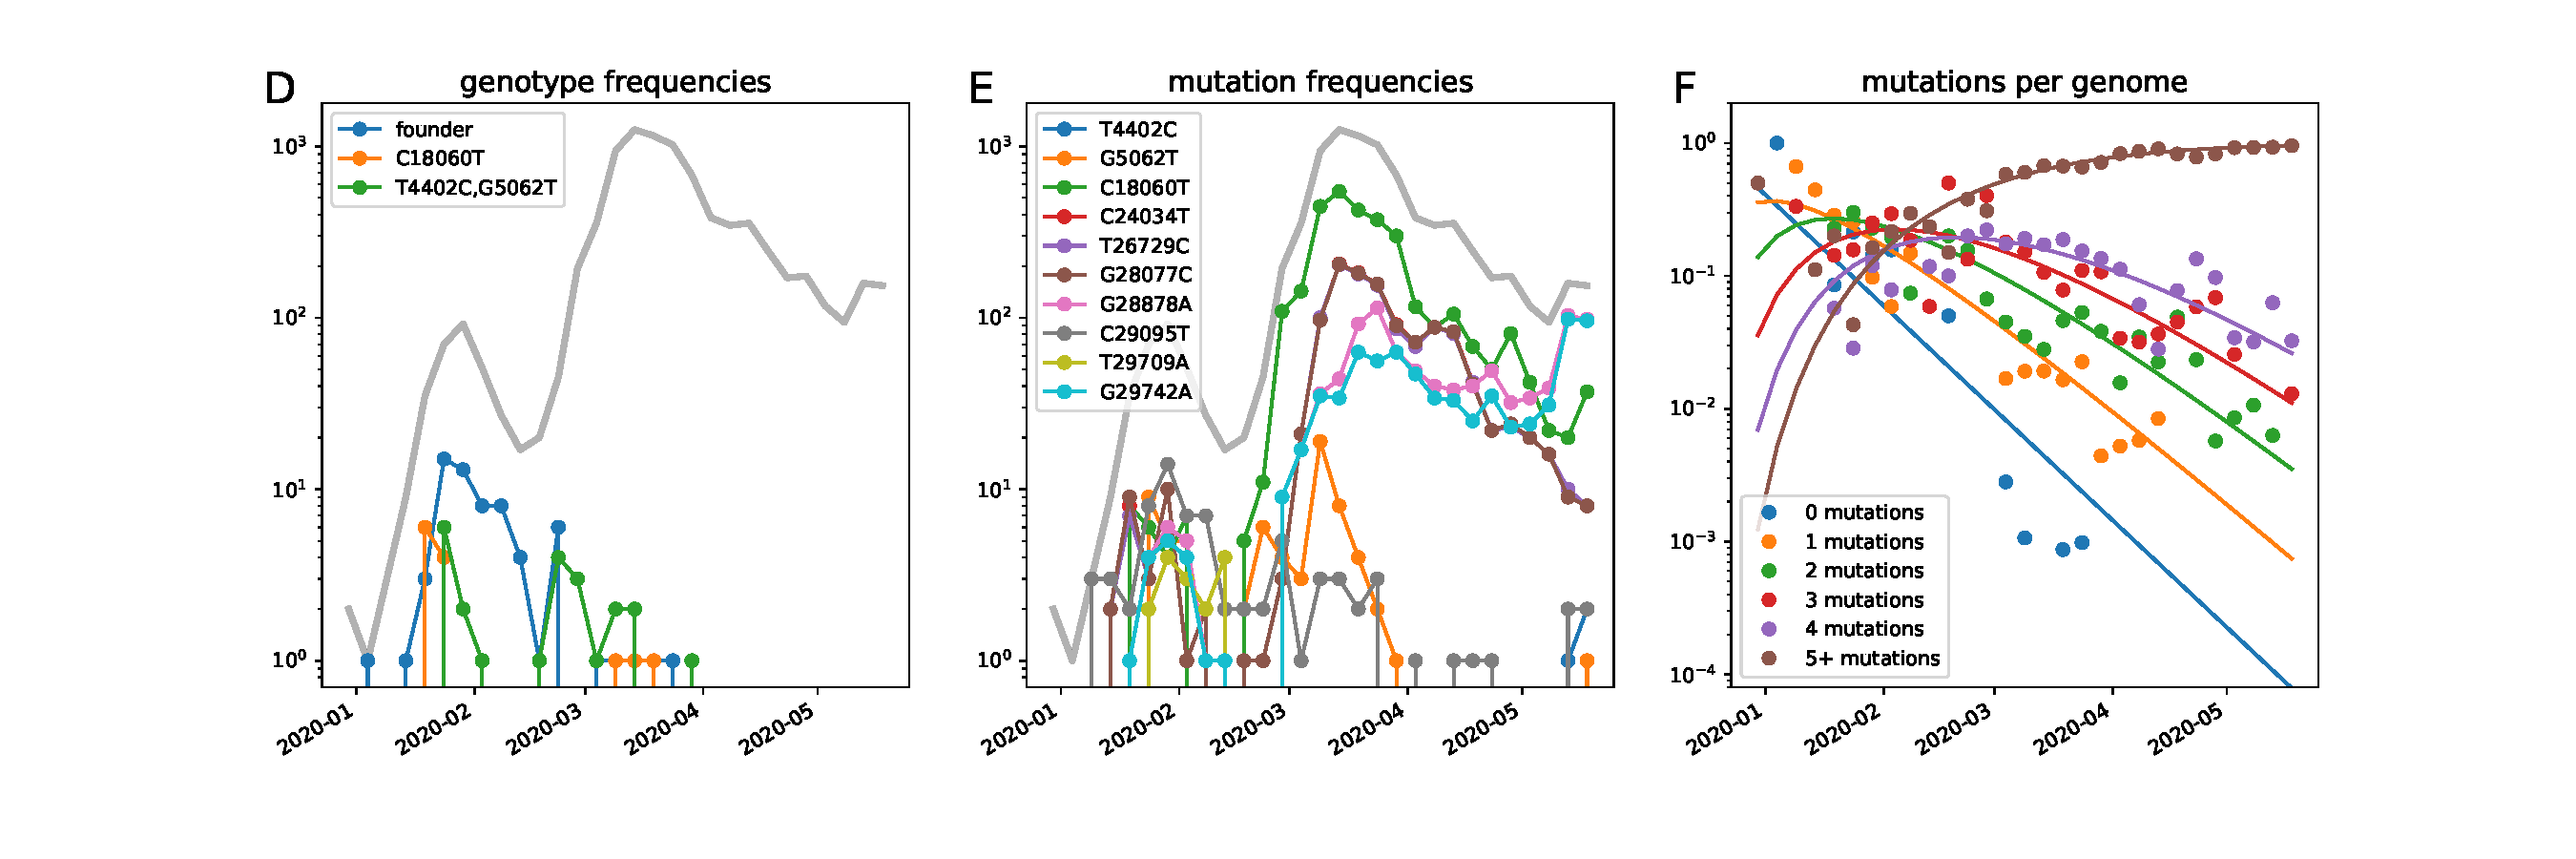
\includegraphics[width=\textwidth]{figures/counts/19B_counts.pdf}
    \caption{{\bf Diversification within clade 19B.}
    \label{fig:19B_counts}}
\end{figure*}

\begin{figure*}[h]
    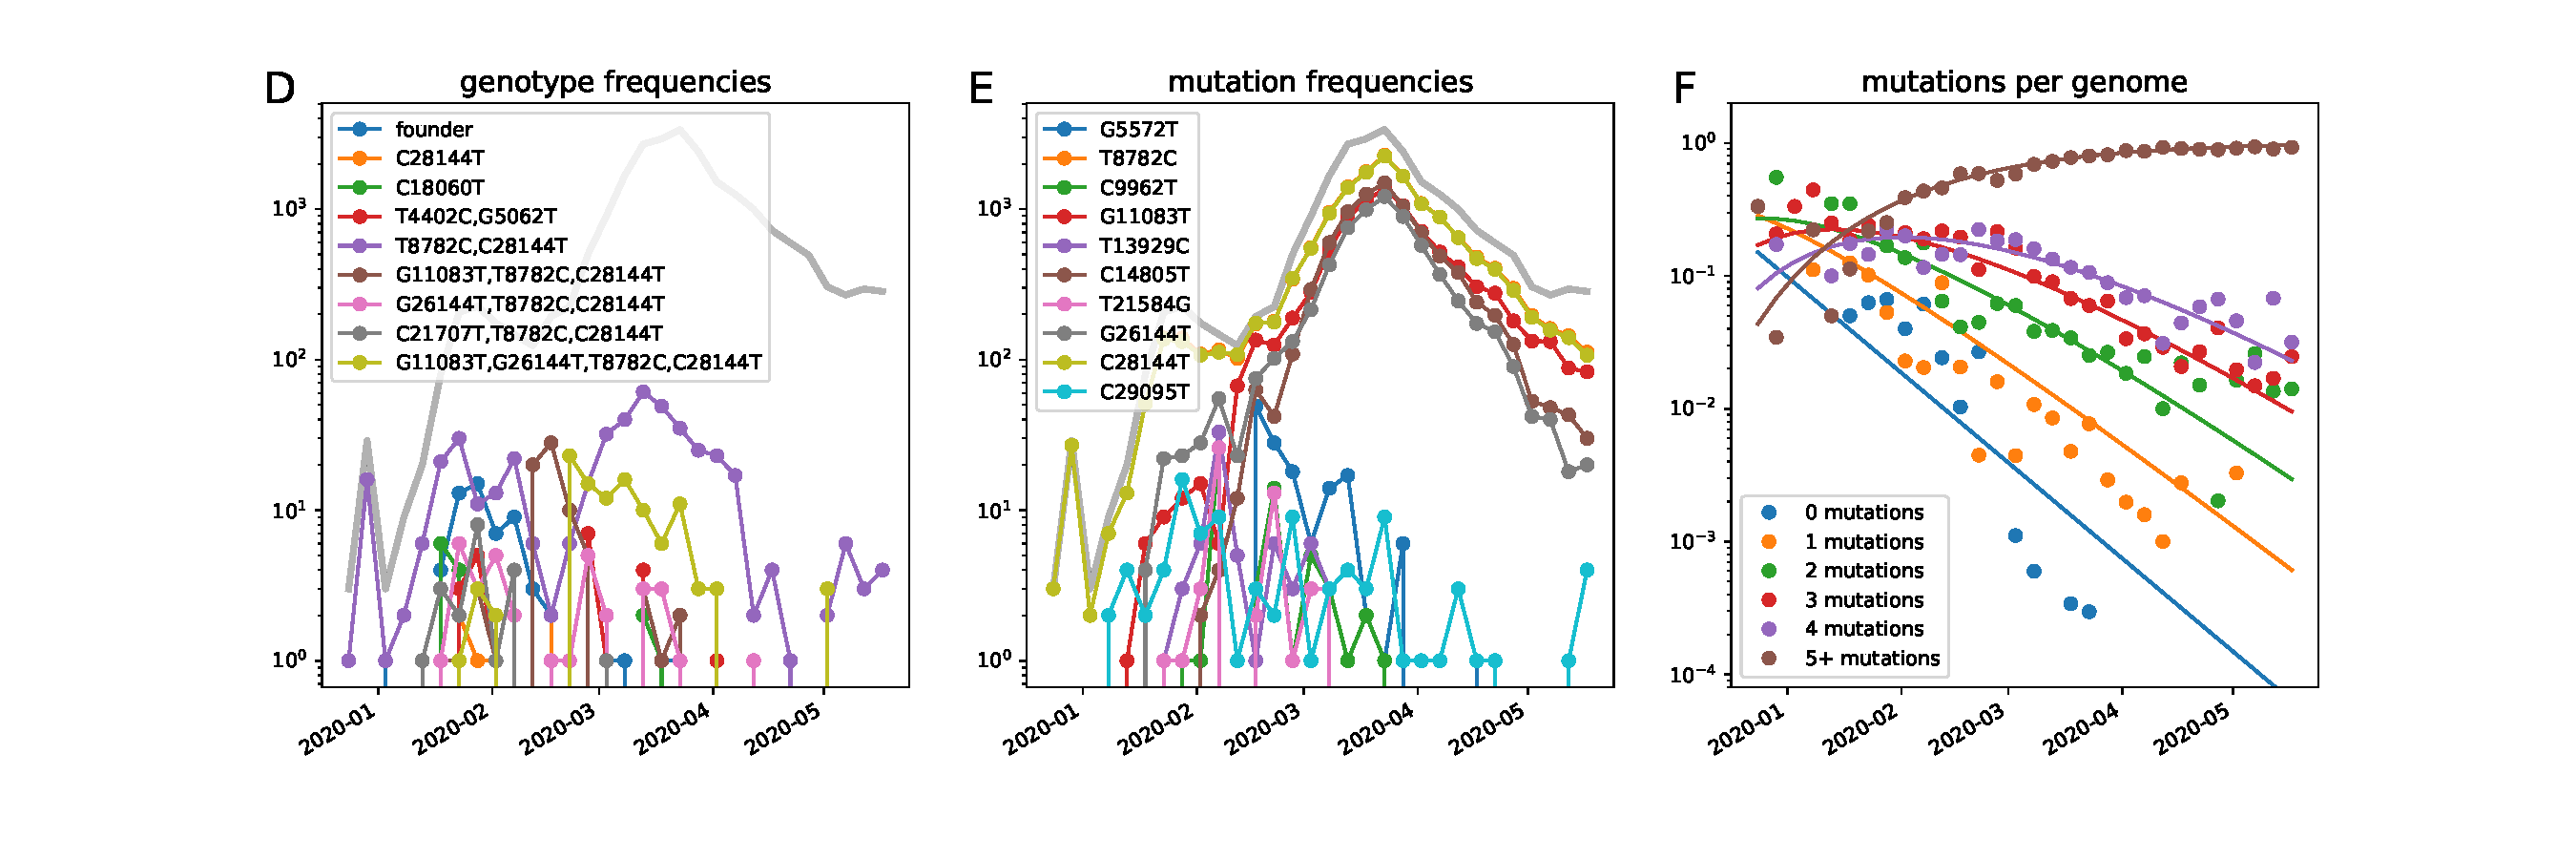
\includegraphics[width=\textwidth]{figures/counts/19B+_counts.pdf}
    \caption{{\bf Diversification within clade 19B+.}
    This figure contains sequences in clades 19 A and B rooted on clade 19B.
    \label{fig:19B+_counts}}
\end{figure*}

\begin{figure*}[h]
    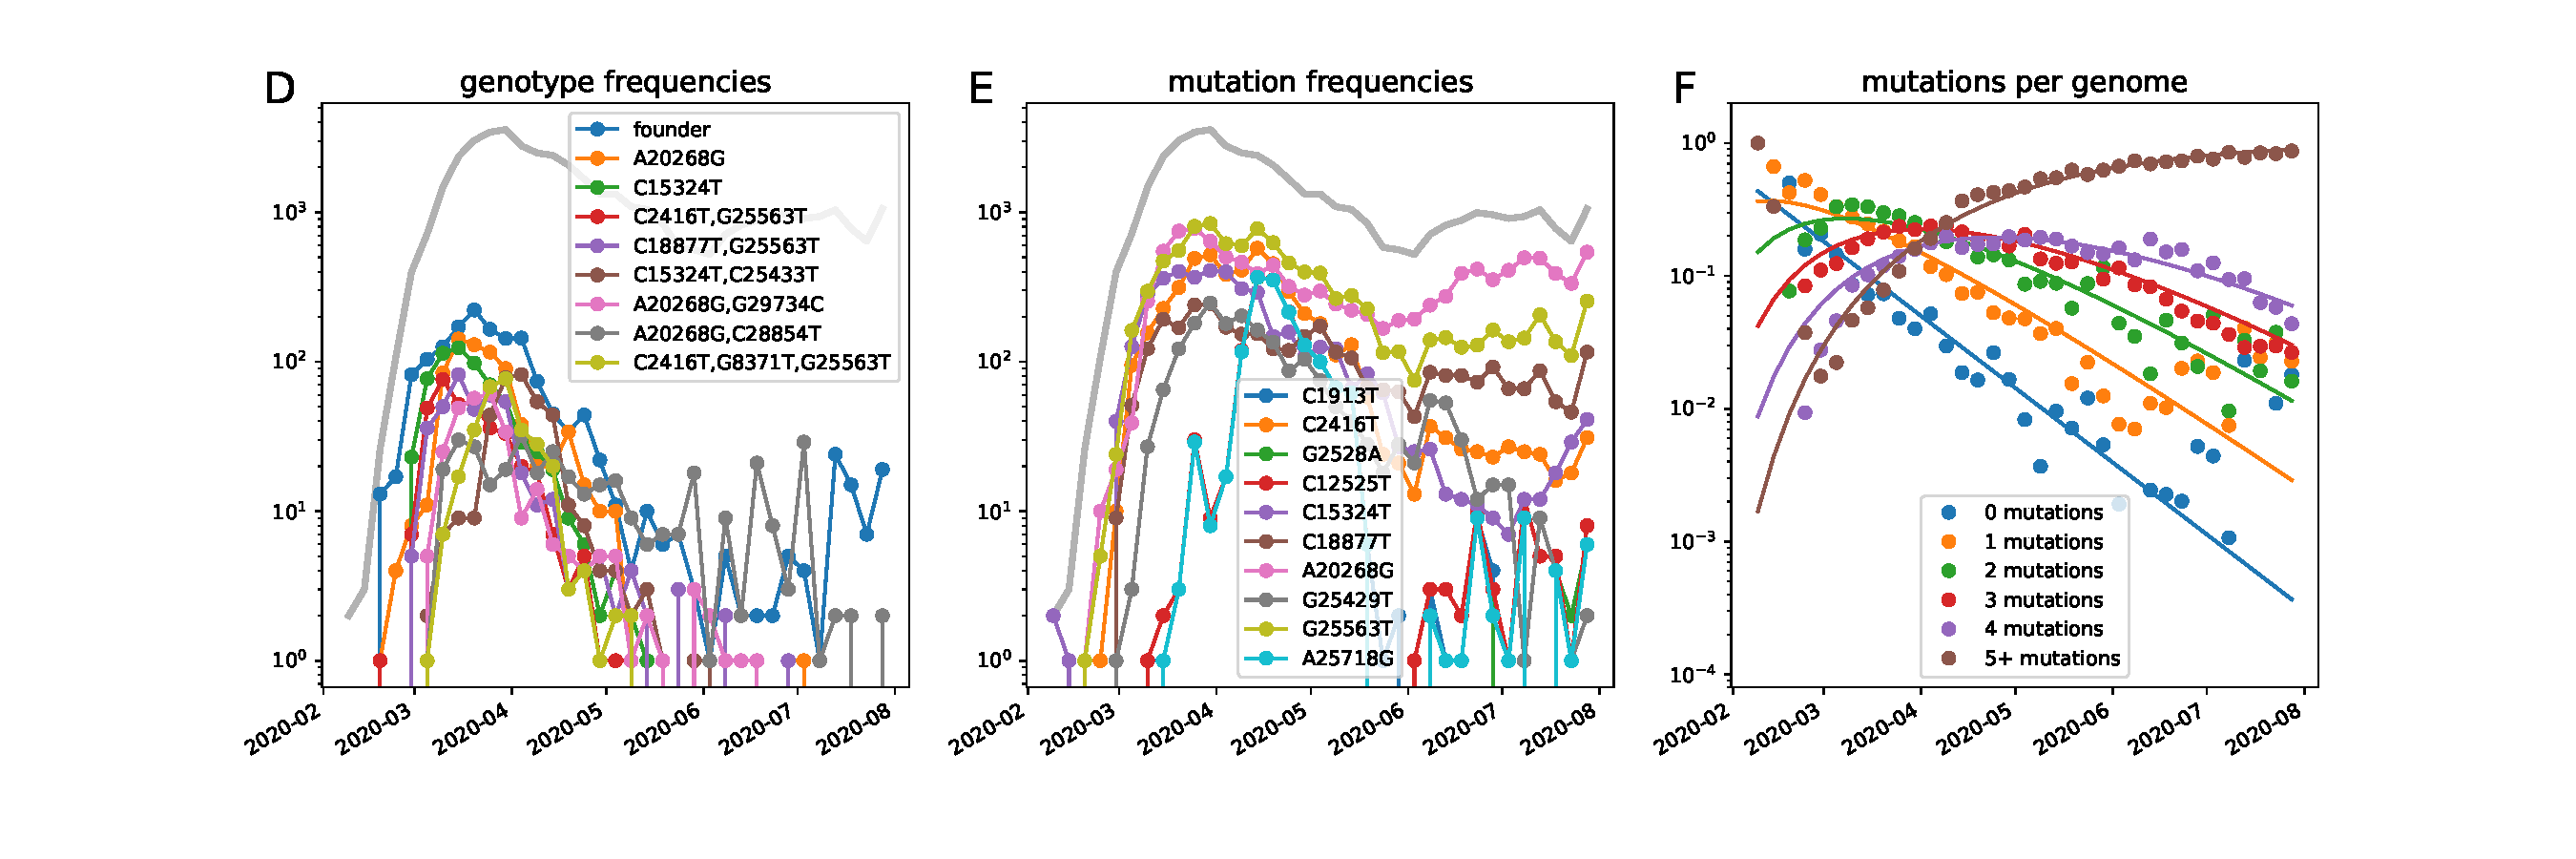
\includegraphics[width=\textwidth]{figures/counts/20A_counts.pdf}
    \caption{{\bf Diversification within clade 20A.}
    \label{fig:20A_counts}}
\end{figure*}

\begin{figure*}[h]
    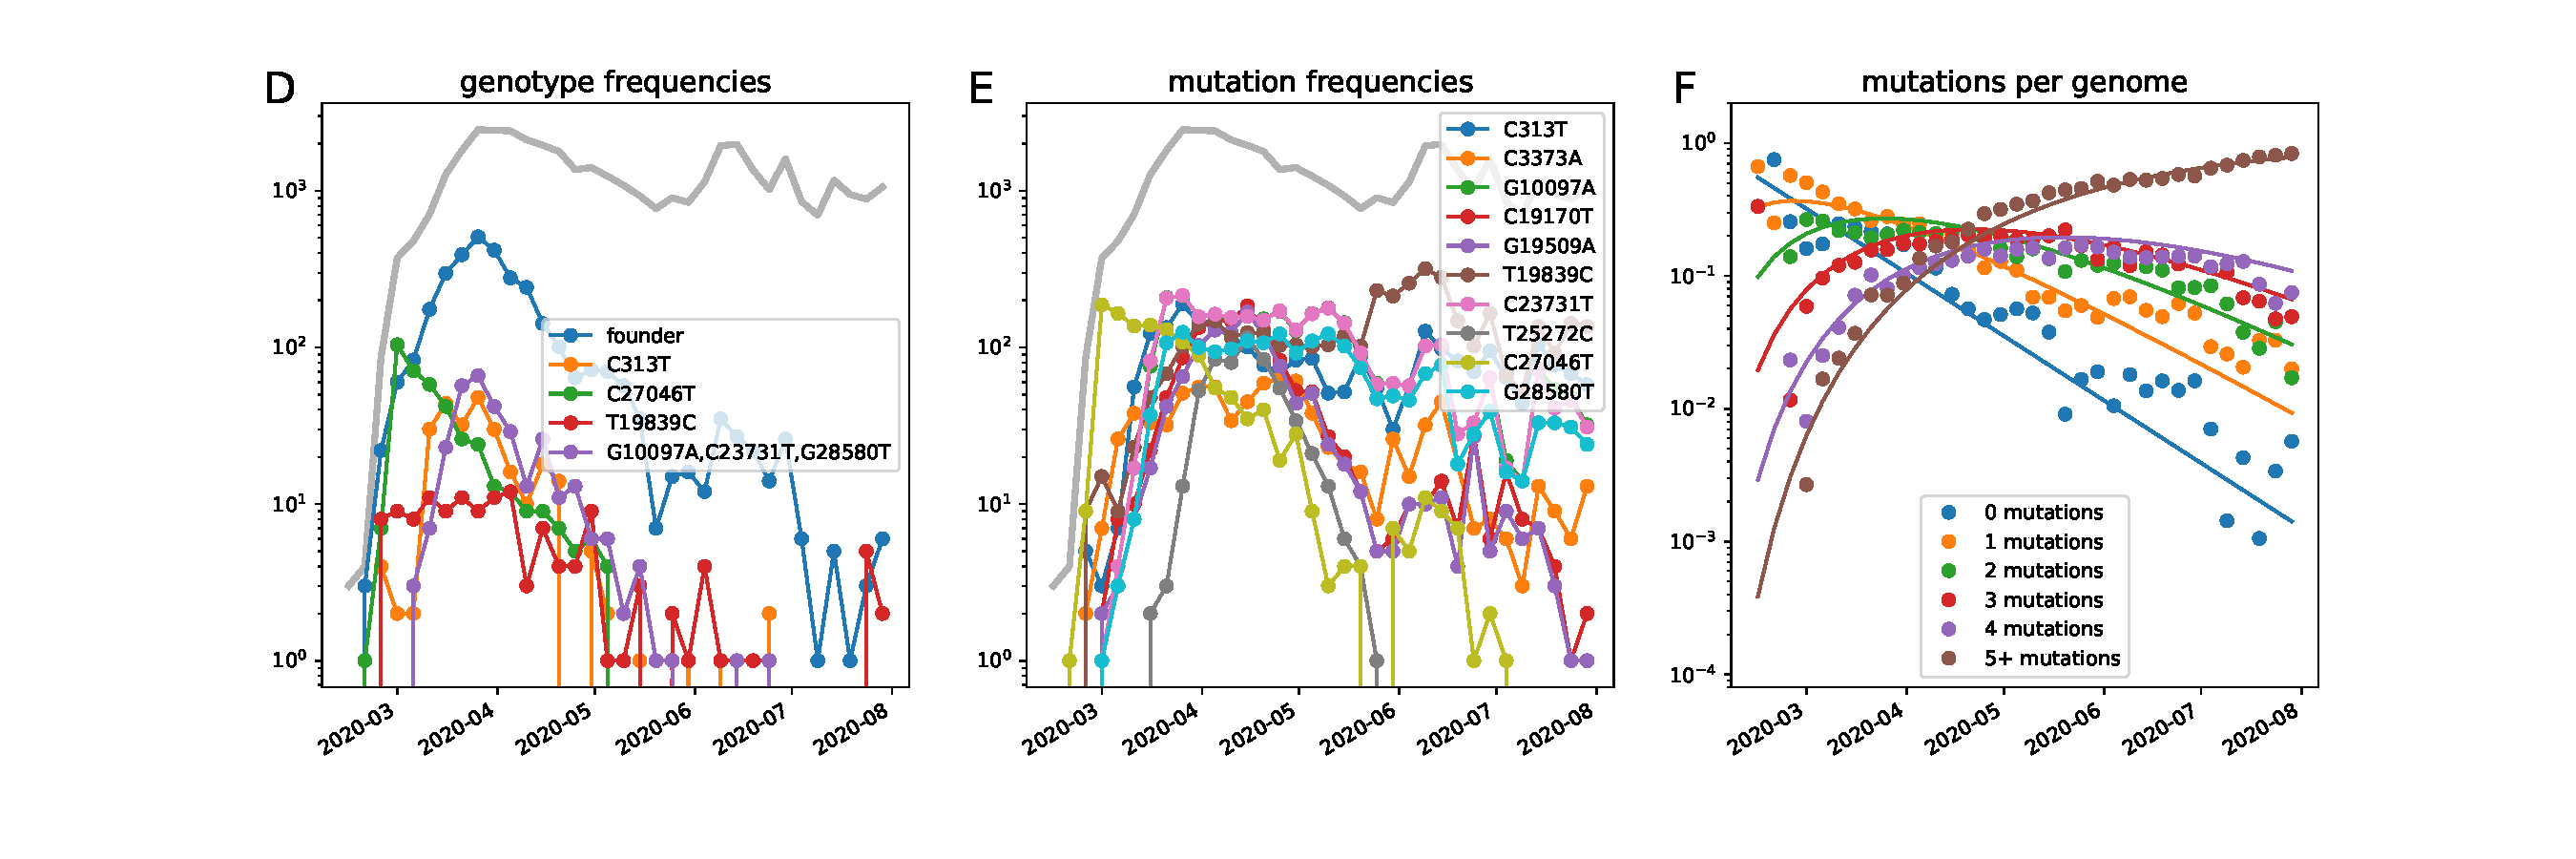
\includegraphics[width=\textwidth]{figures/counts/20B_counts.pdf}
    \caption{{\bf Diversification within clade 20B.}
    \label{fig:20B_counts}}
\end{figure*}

\begin{figure*}[h]
    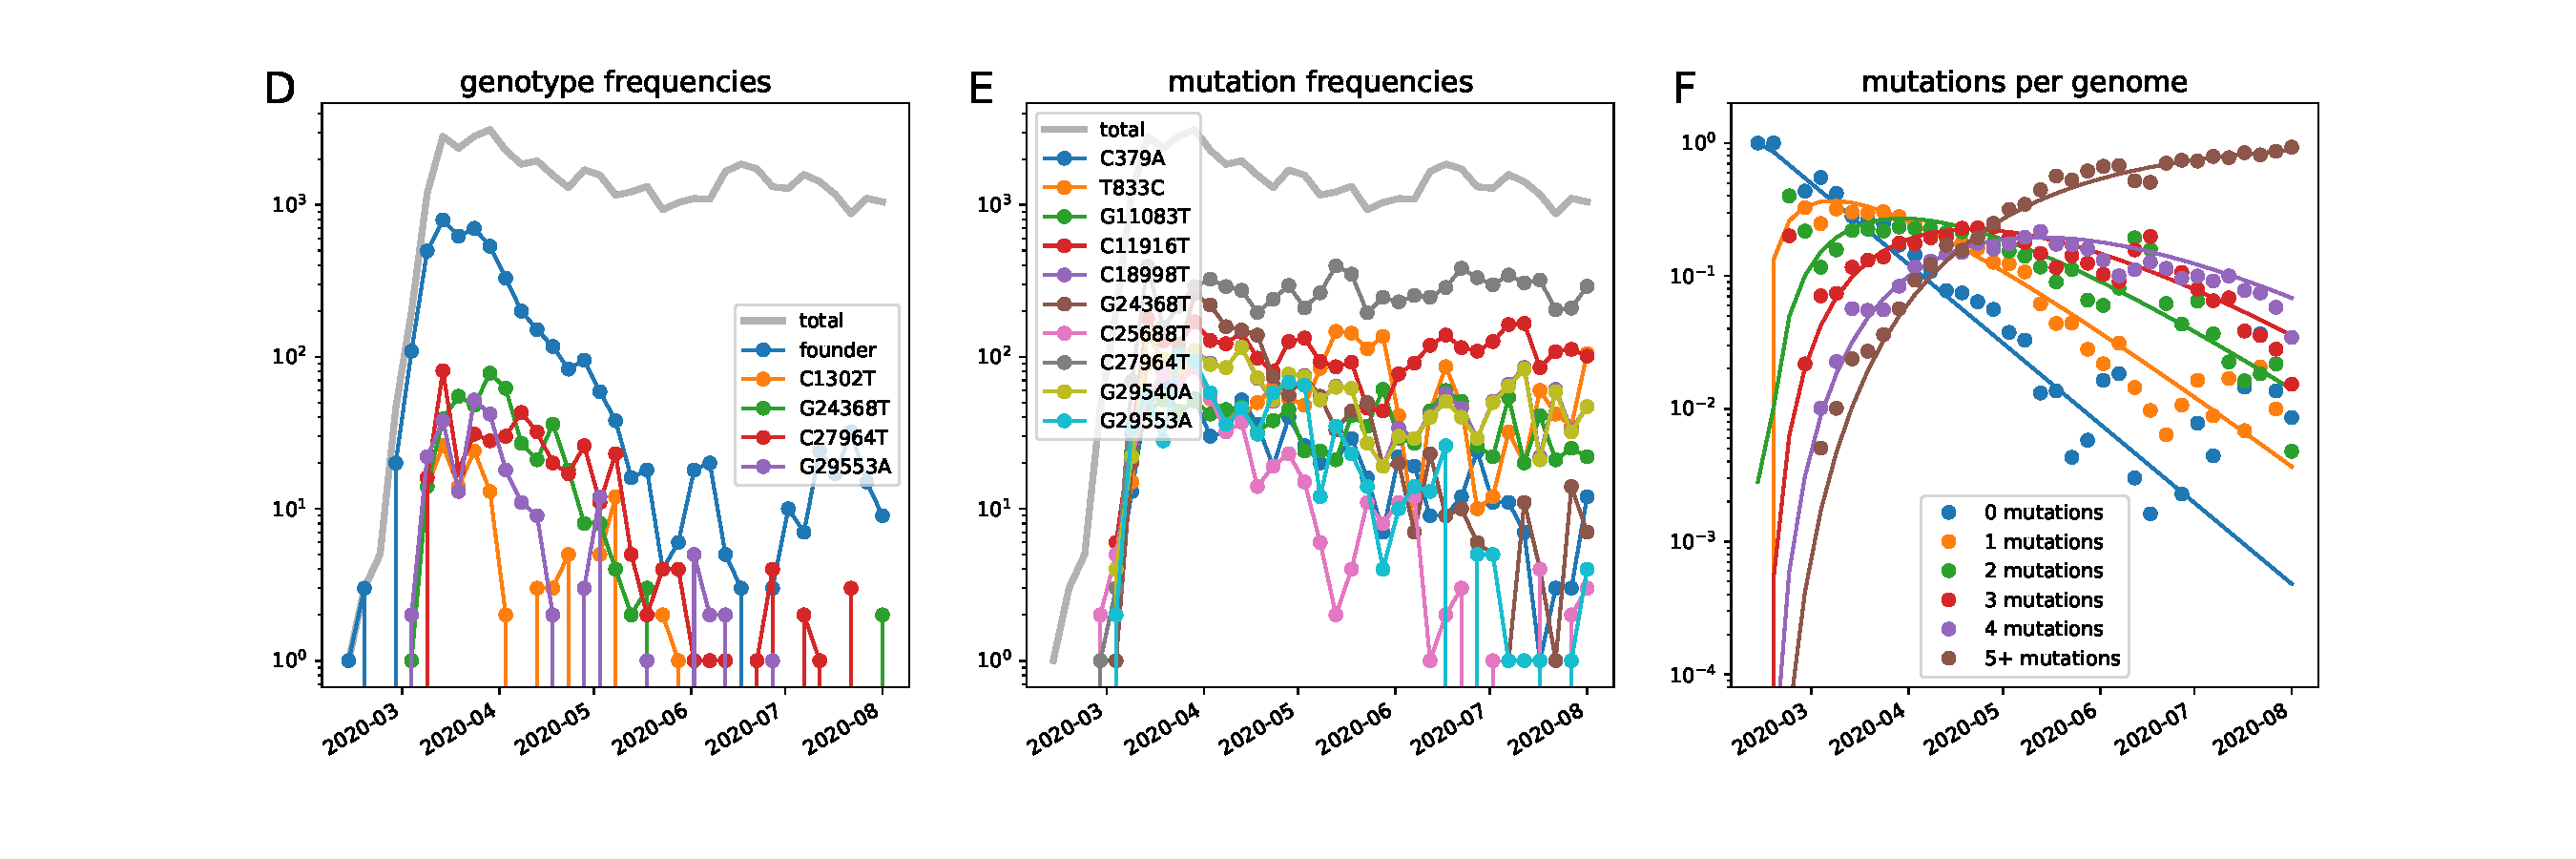
\includegraphics[width=\textwidth]{figures/counts/20C_counts.pdf}
    \caption{{\bf Diversification within clade 20C.}
    \label{fig:20C_counts}}
\end{figure*}


\begin{figure*}[h]
    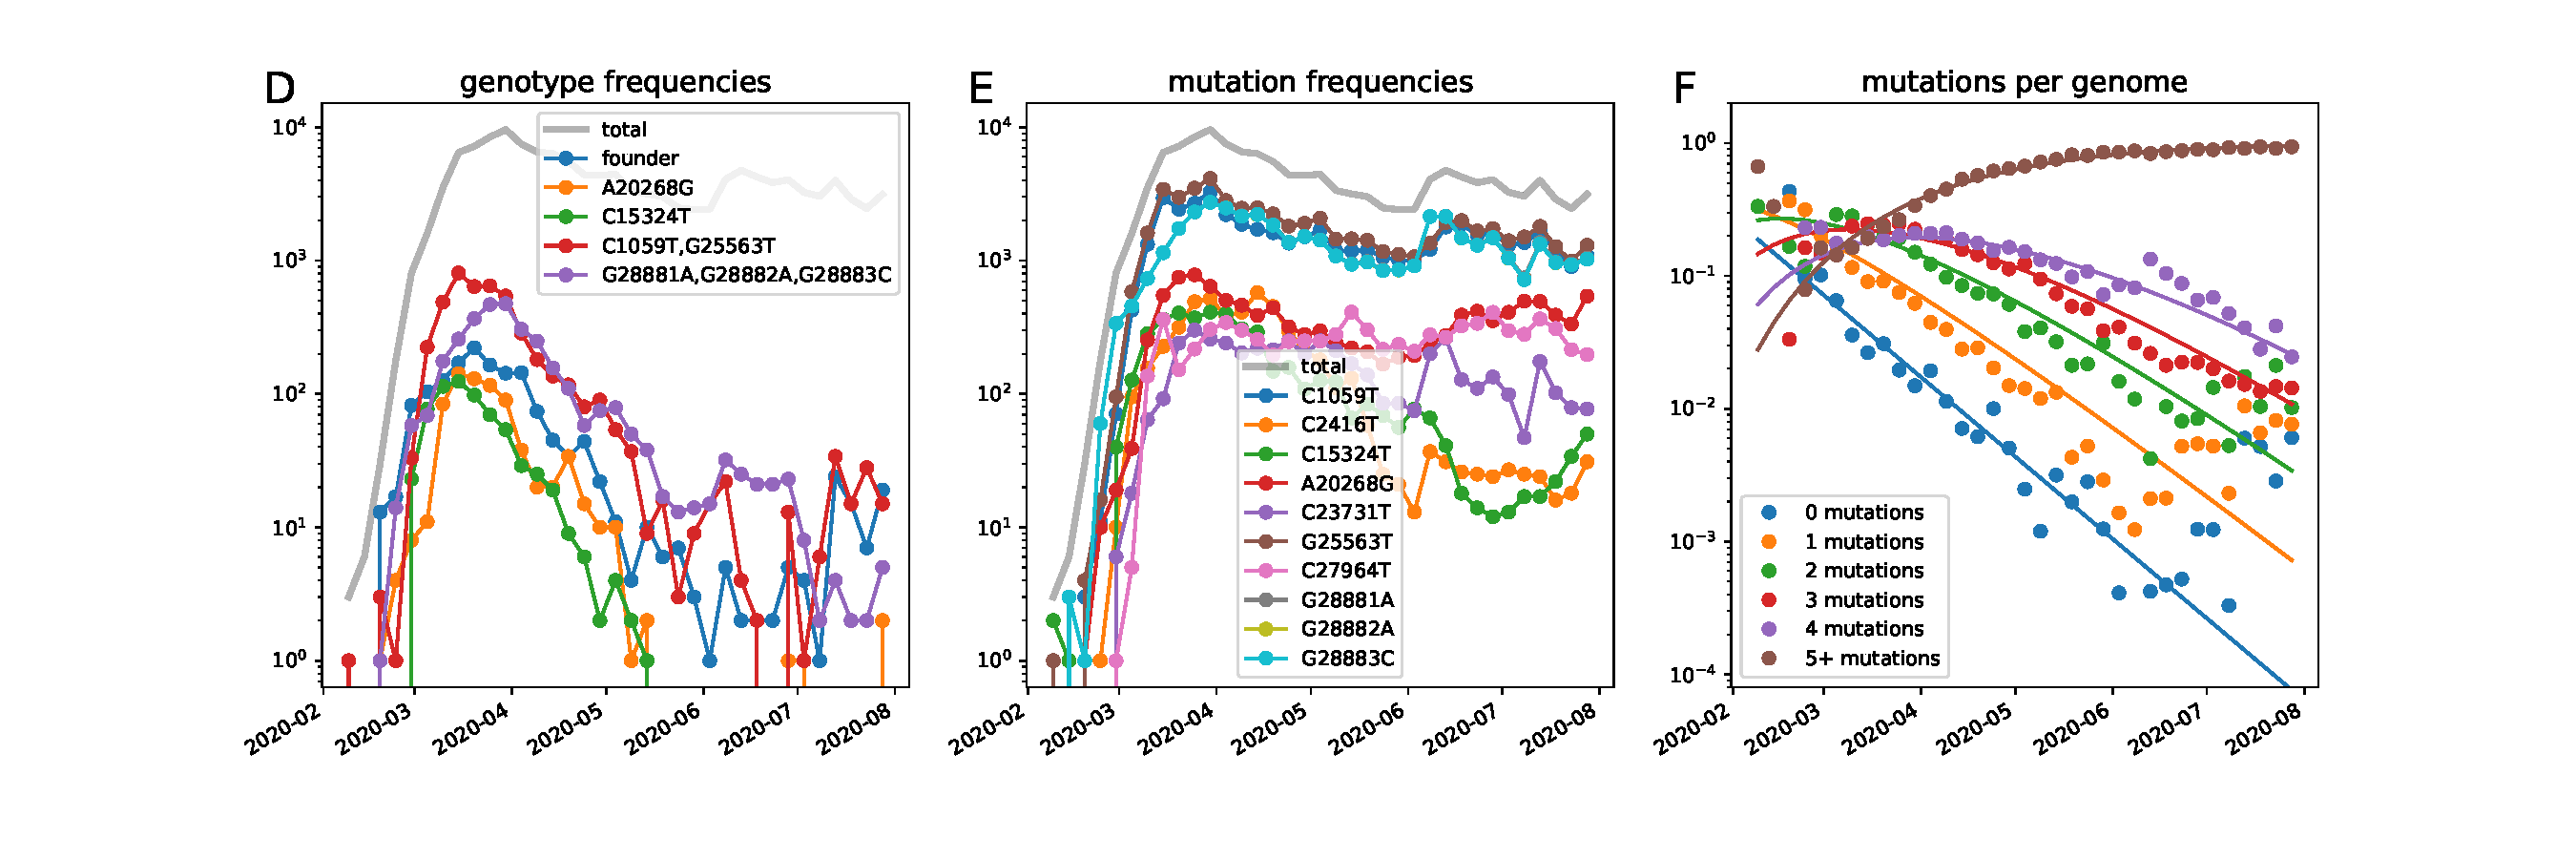
\includegraphics[width=\textwidth]{figures/counts/20A+_counts.pdf}
    \caption{{\bf Diversification within clade 20A+.}
    This figure contains sequences in clades 20A,B,C,D rooted on clade 20A.
    \label{fig:20A+_counts}}
\end{figure*}



\begin{figure*}[h]
    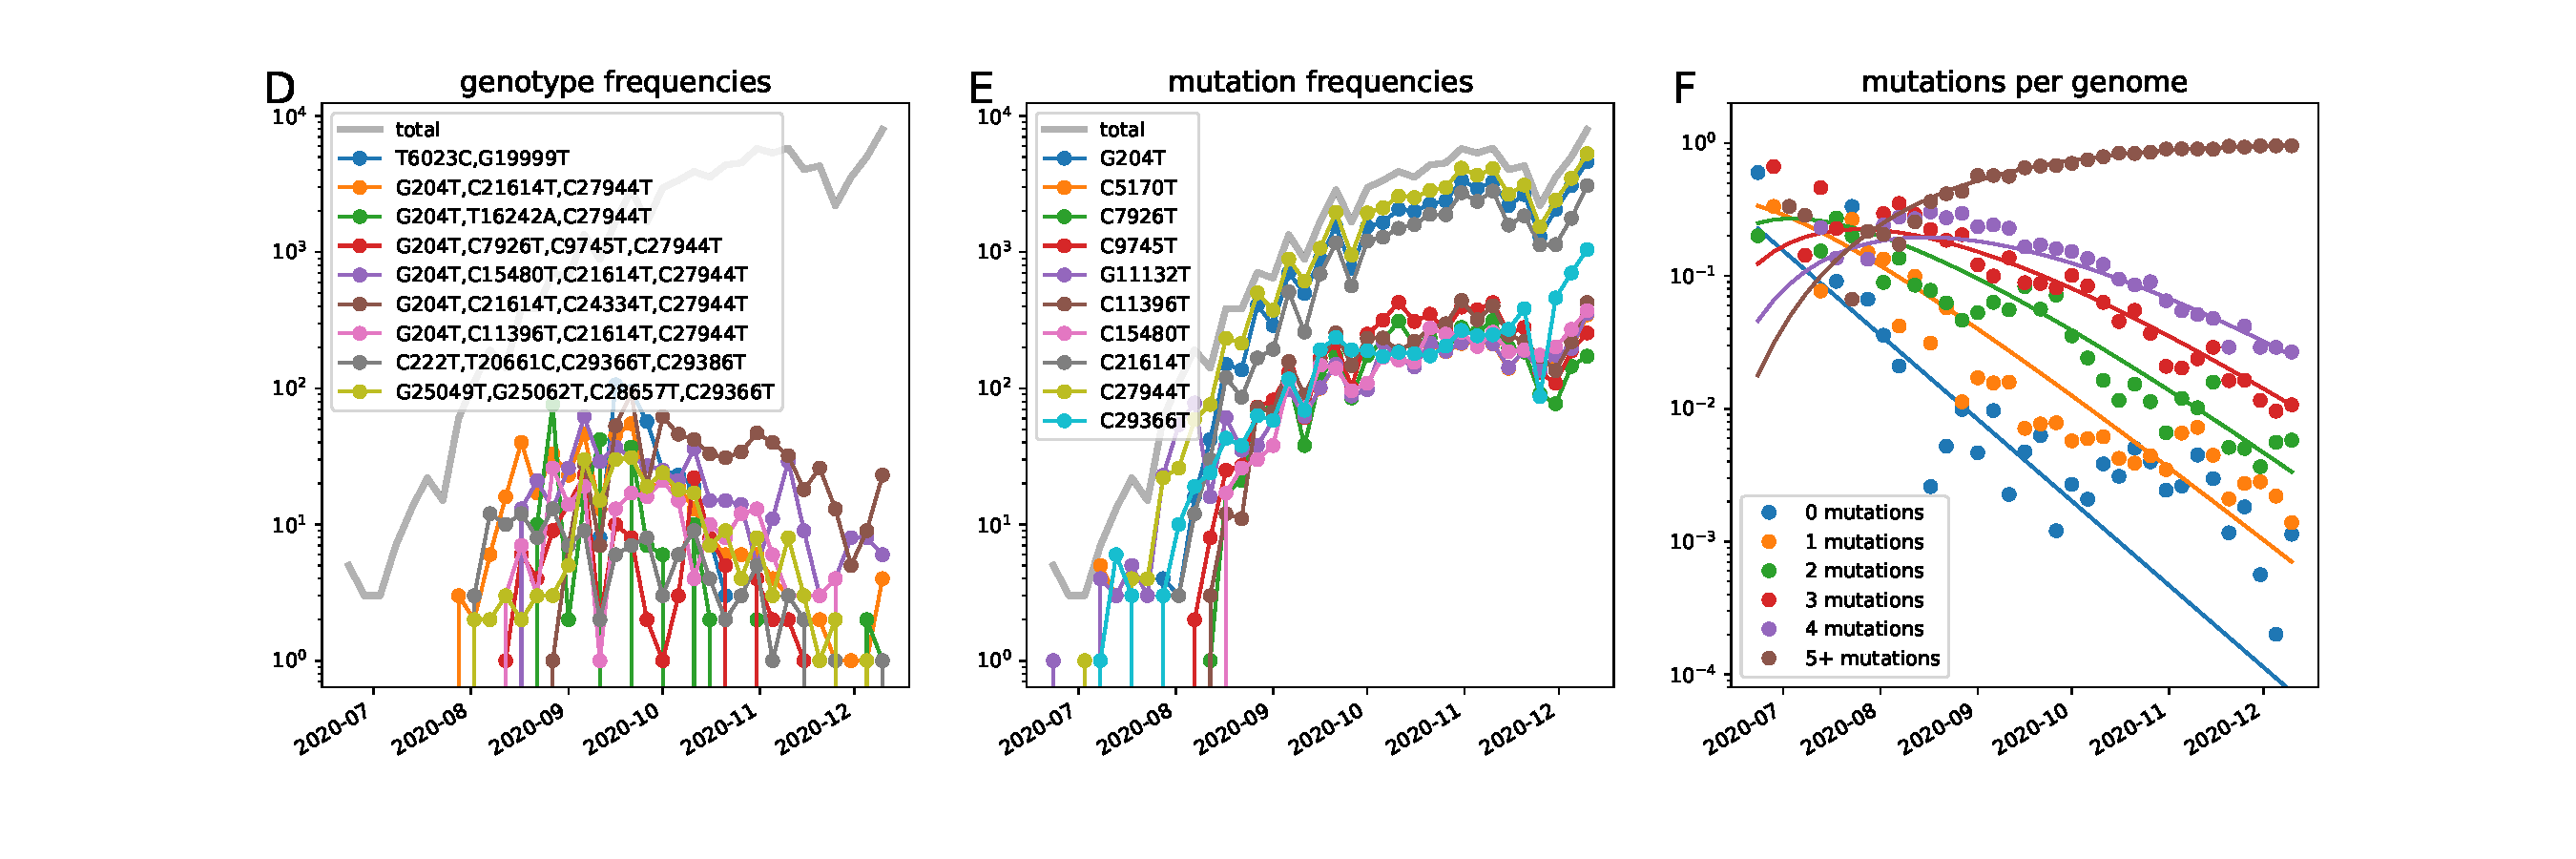
\includegraphics[width=\textwidth]{figures/counts/20E_counts.pdf}
    \caption{{\bf Diversification within clade 20E.}
    \label{fig:20E_counts}}
\end{figure*}

\begin{figure*}[h]
    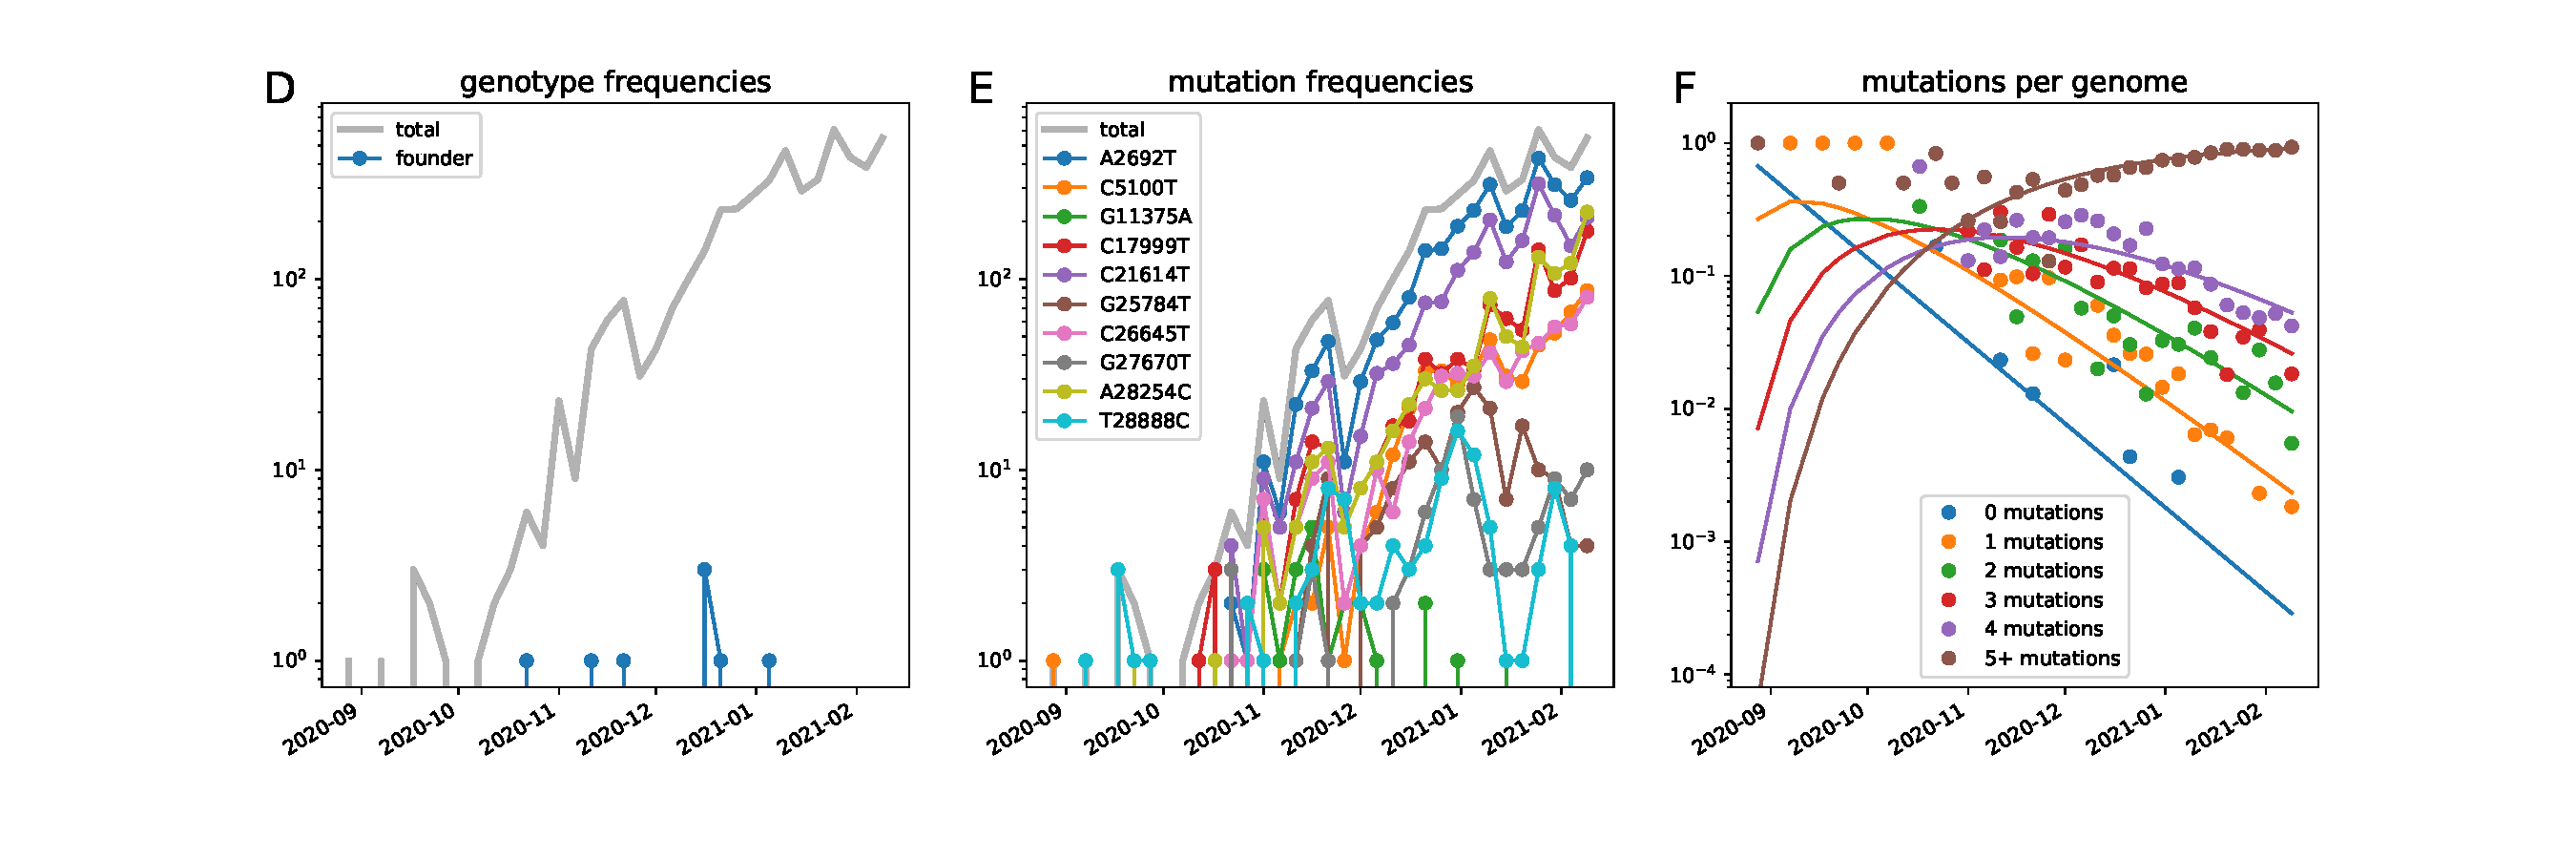
\includegraphics[width=\textwidth]{figures/counts/20H_counts.pdf}
    \caption{{\bf Diversification within clade 20H (Beta).}
    \label{fig:20H_counts}}
\end{figure*}

\begin{figure*}[h]
    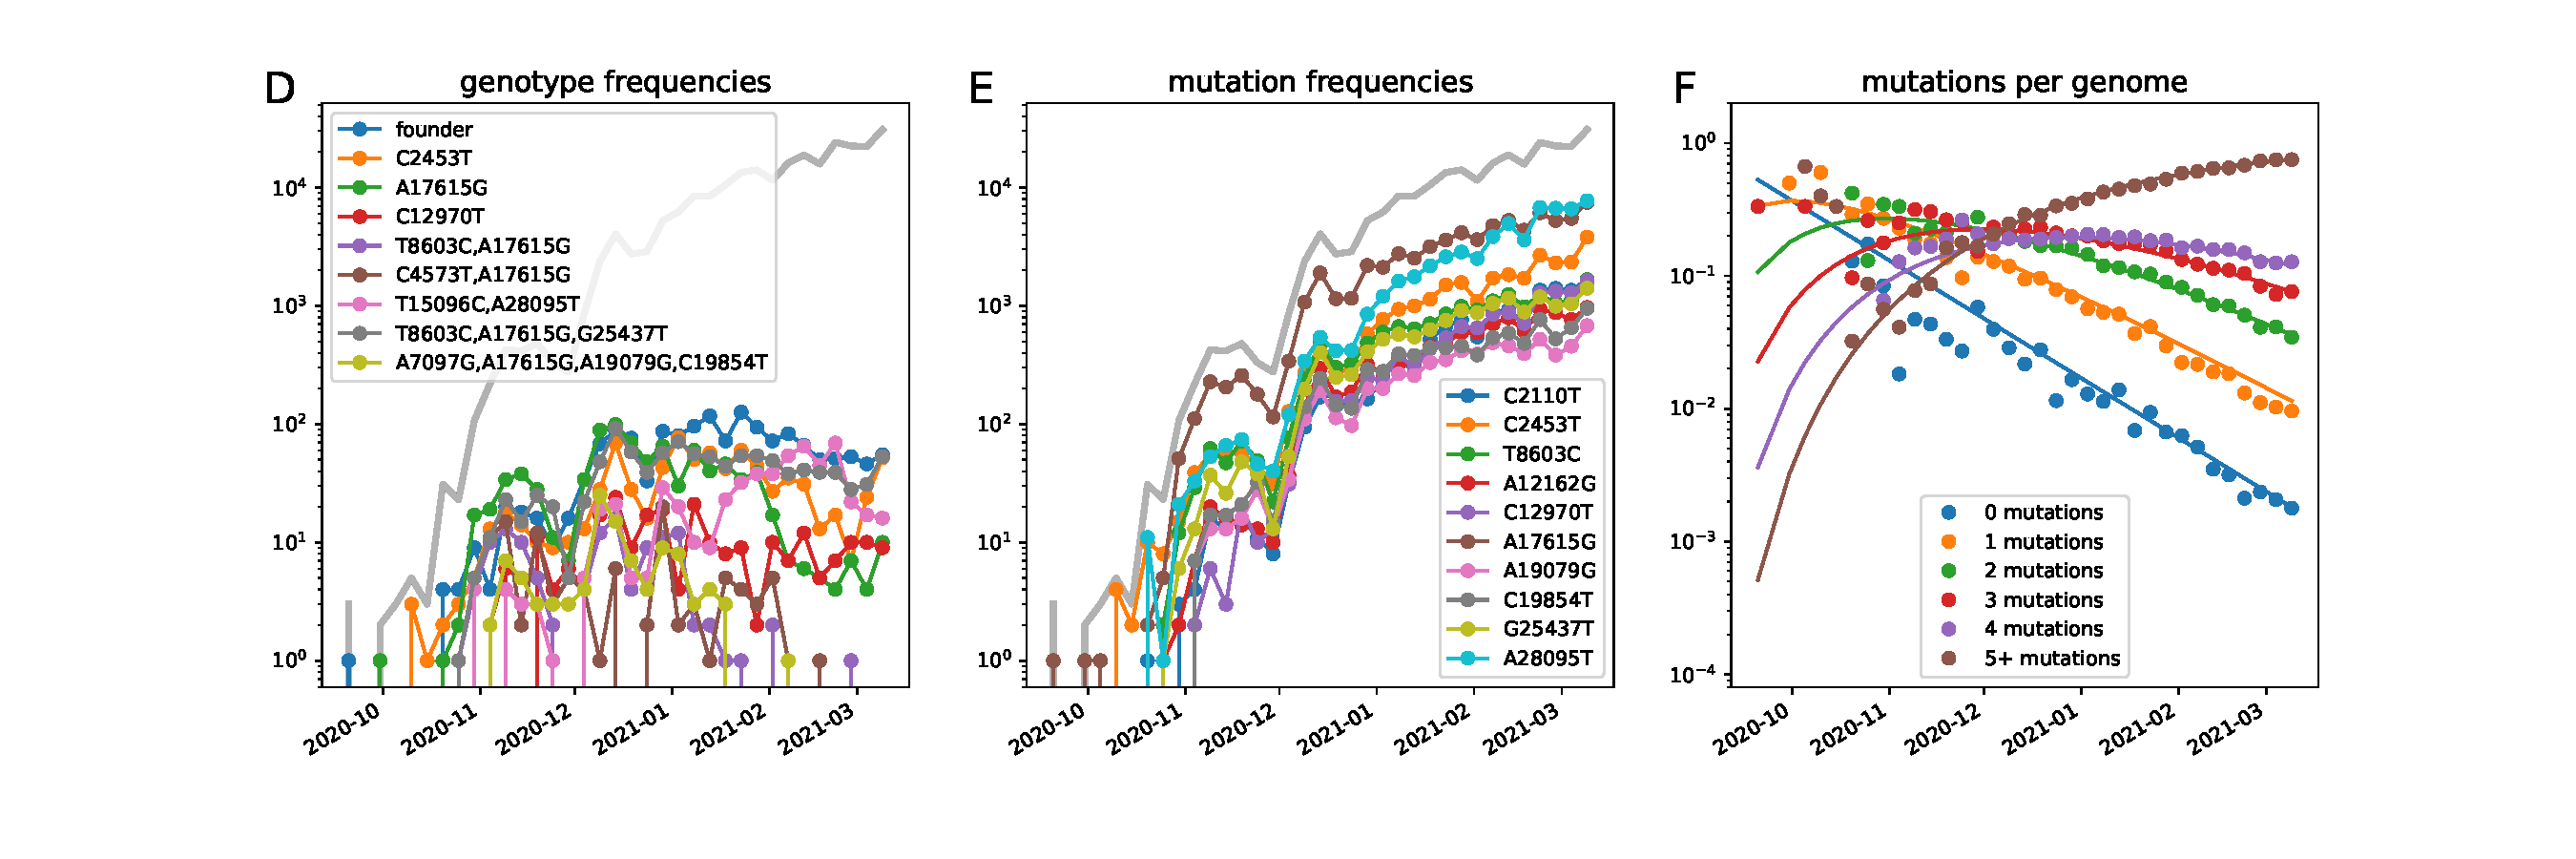
\includegraphics[width=\textwidth]{figures/counts/20I_counts.pdf}
    \caption{{\bf Diversification within clade 20I (Alpha).}
    \label{fig:20I_counts}}
\end{figure*}

\begin{figure*}[h]
    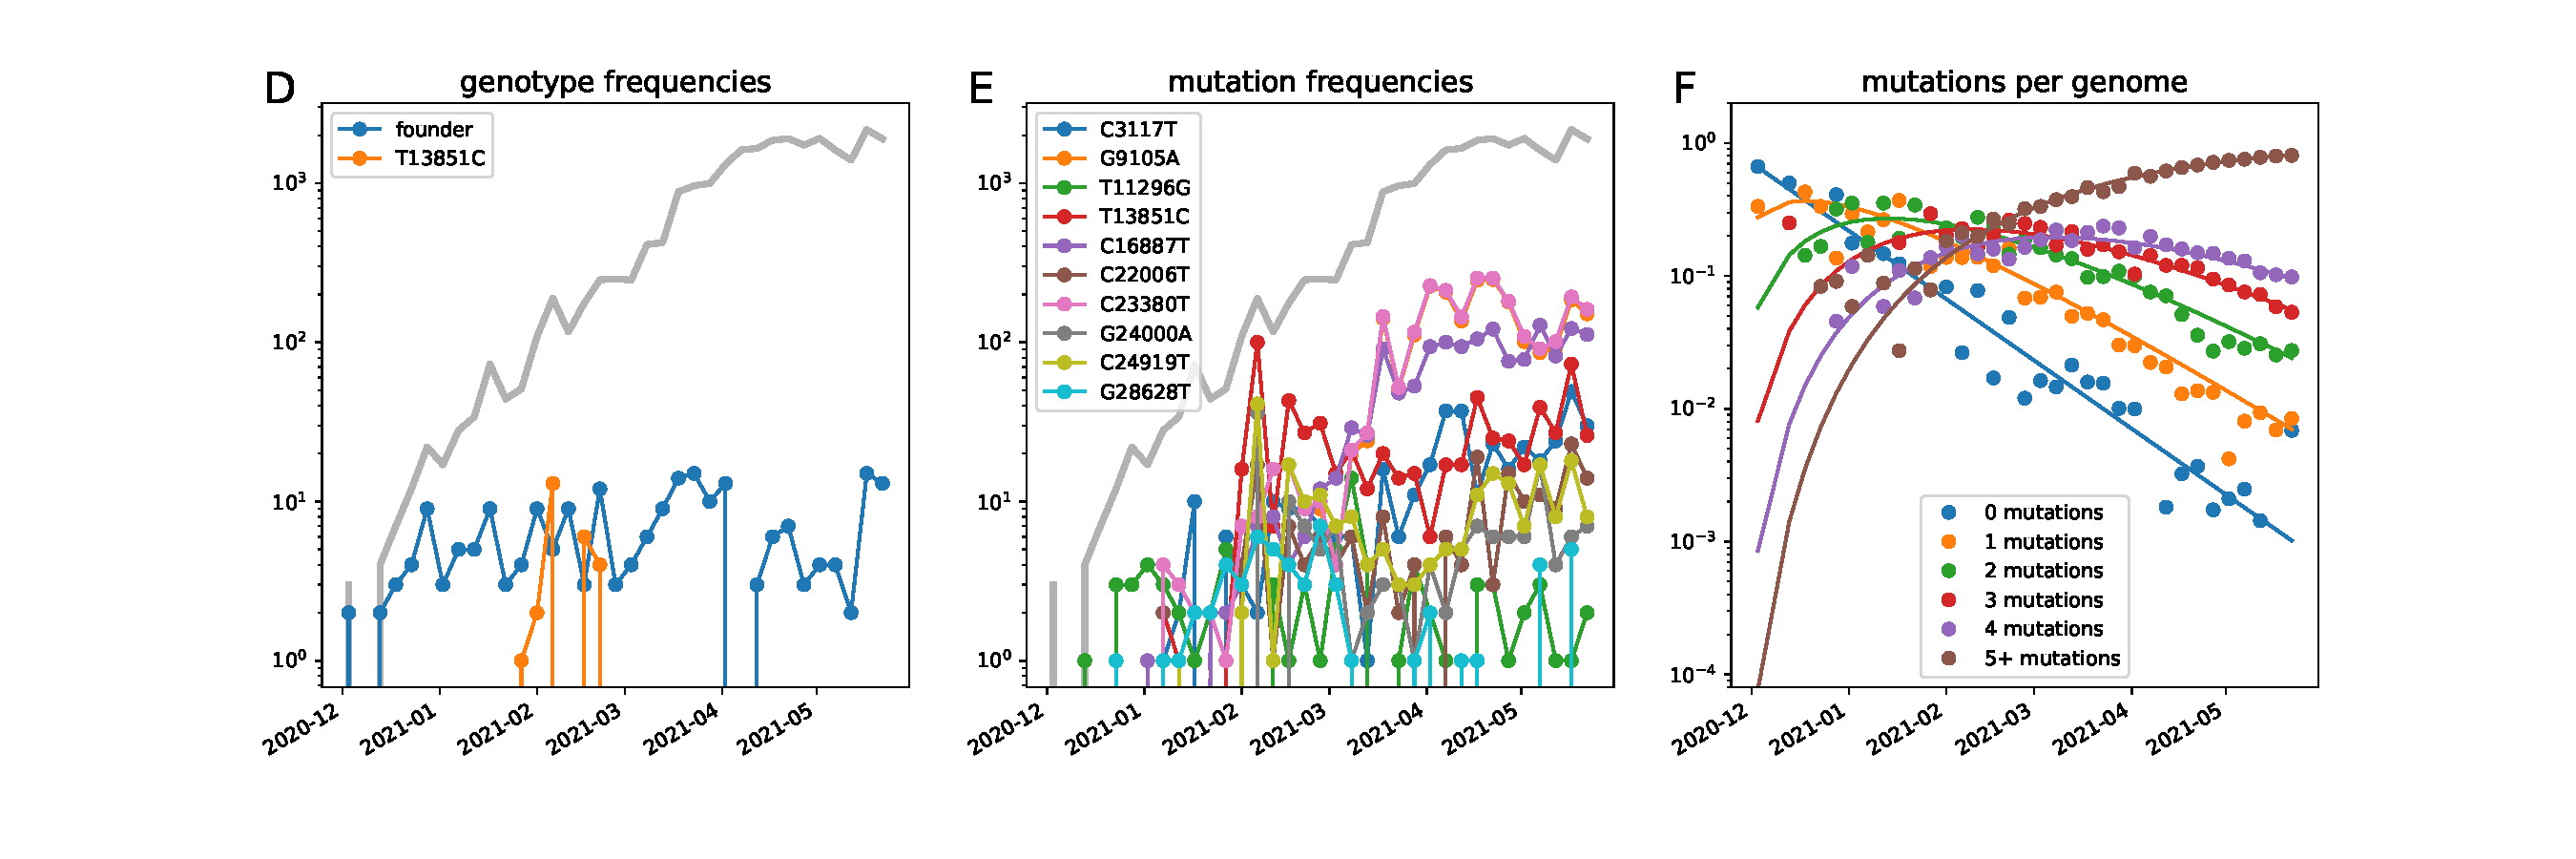
\includegraphics[width=\textwidth]{figures/counts/20J_counts.pdf}
    \caption{{\bf Diversification within clade 20J (Gamma).}
    \label{fig:20J_counts}}
\end{figure*}


\begin{figure*}[h]
    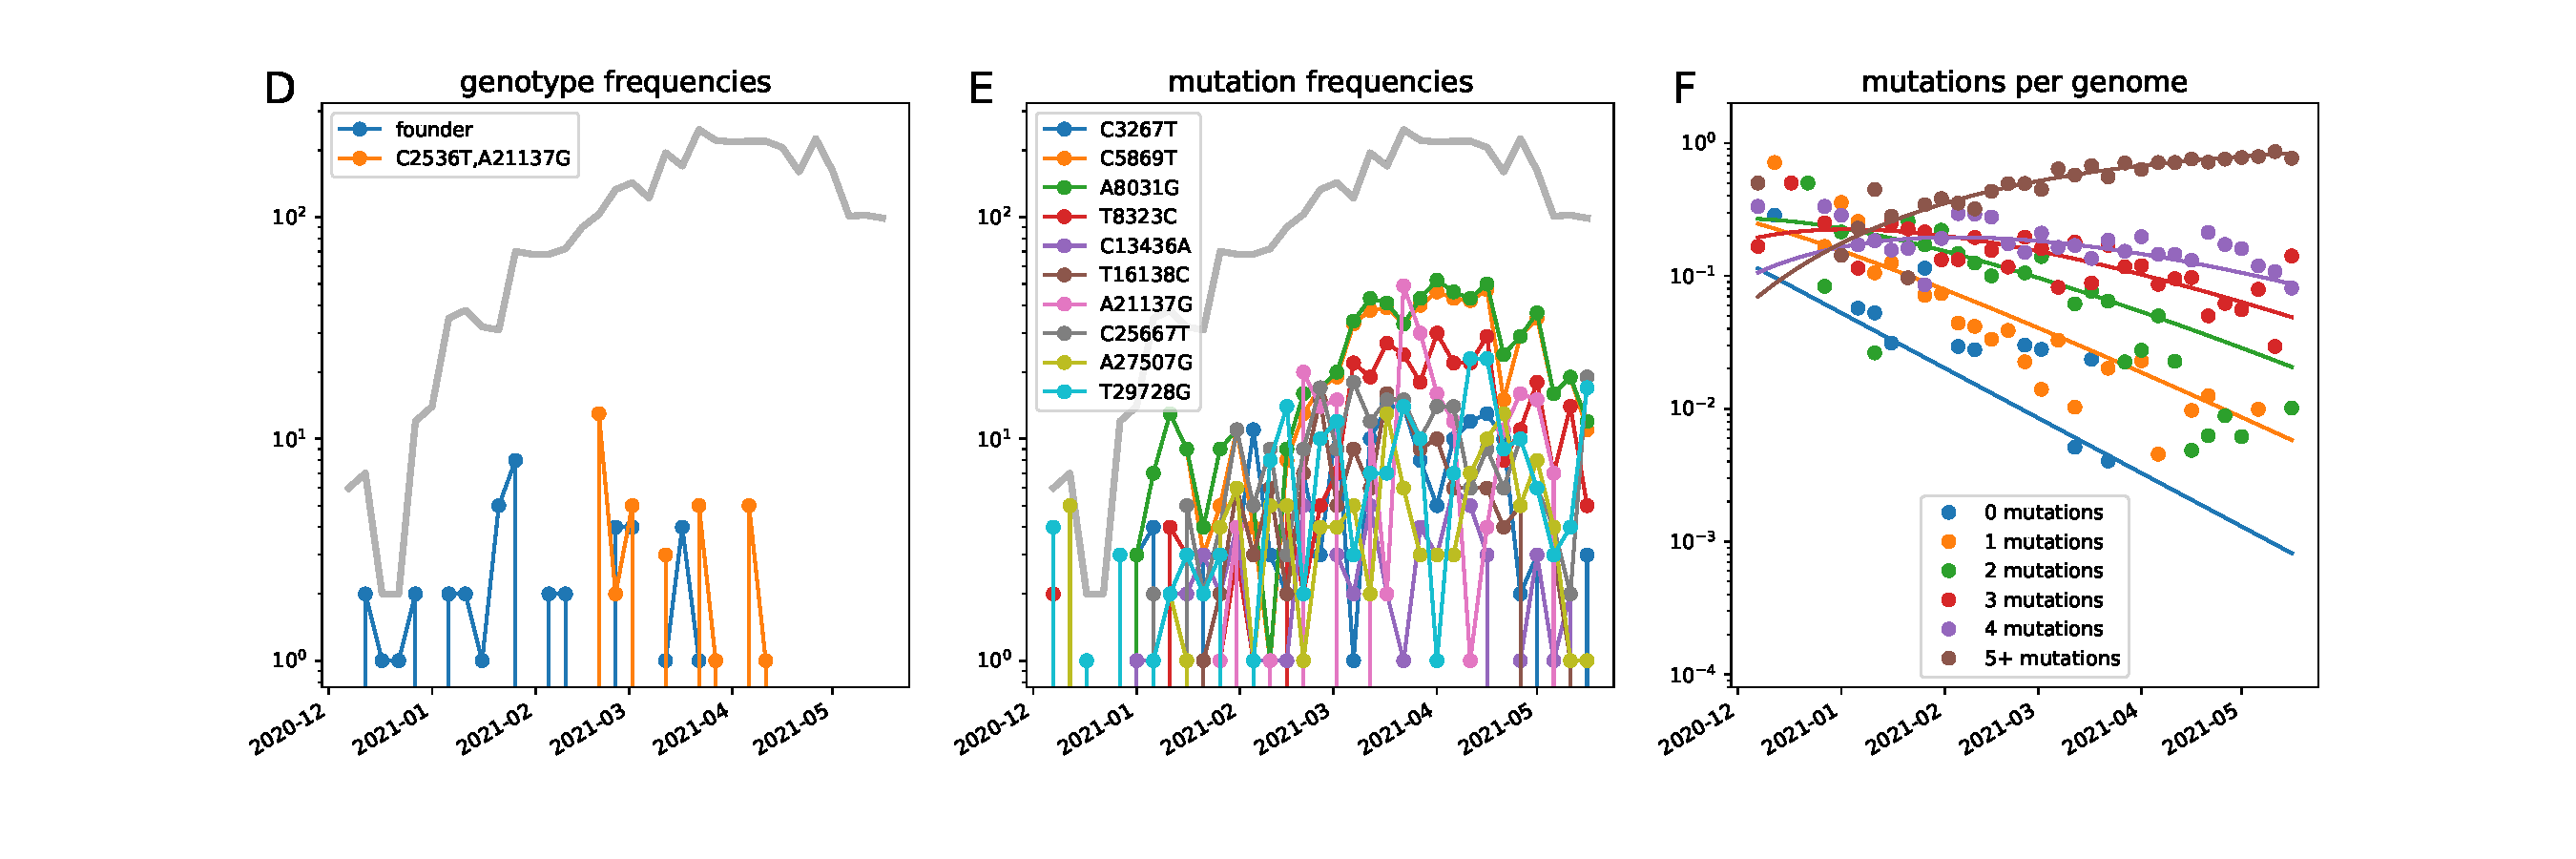
\includegraphics[width=\textwidth]{figures/counts/21D_counts.pdf}
    \caption{{\bf Diversification within clade 21D (Eta).}
    \label{fig:21D_counts}}
\end{figure*}


\begin{figure*}[h]
    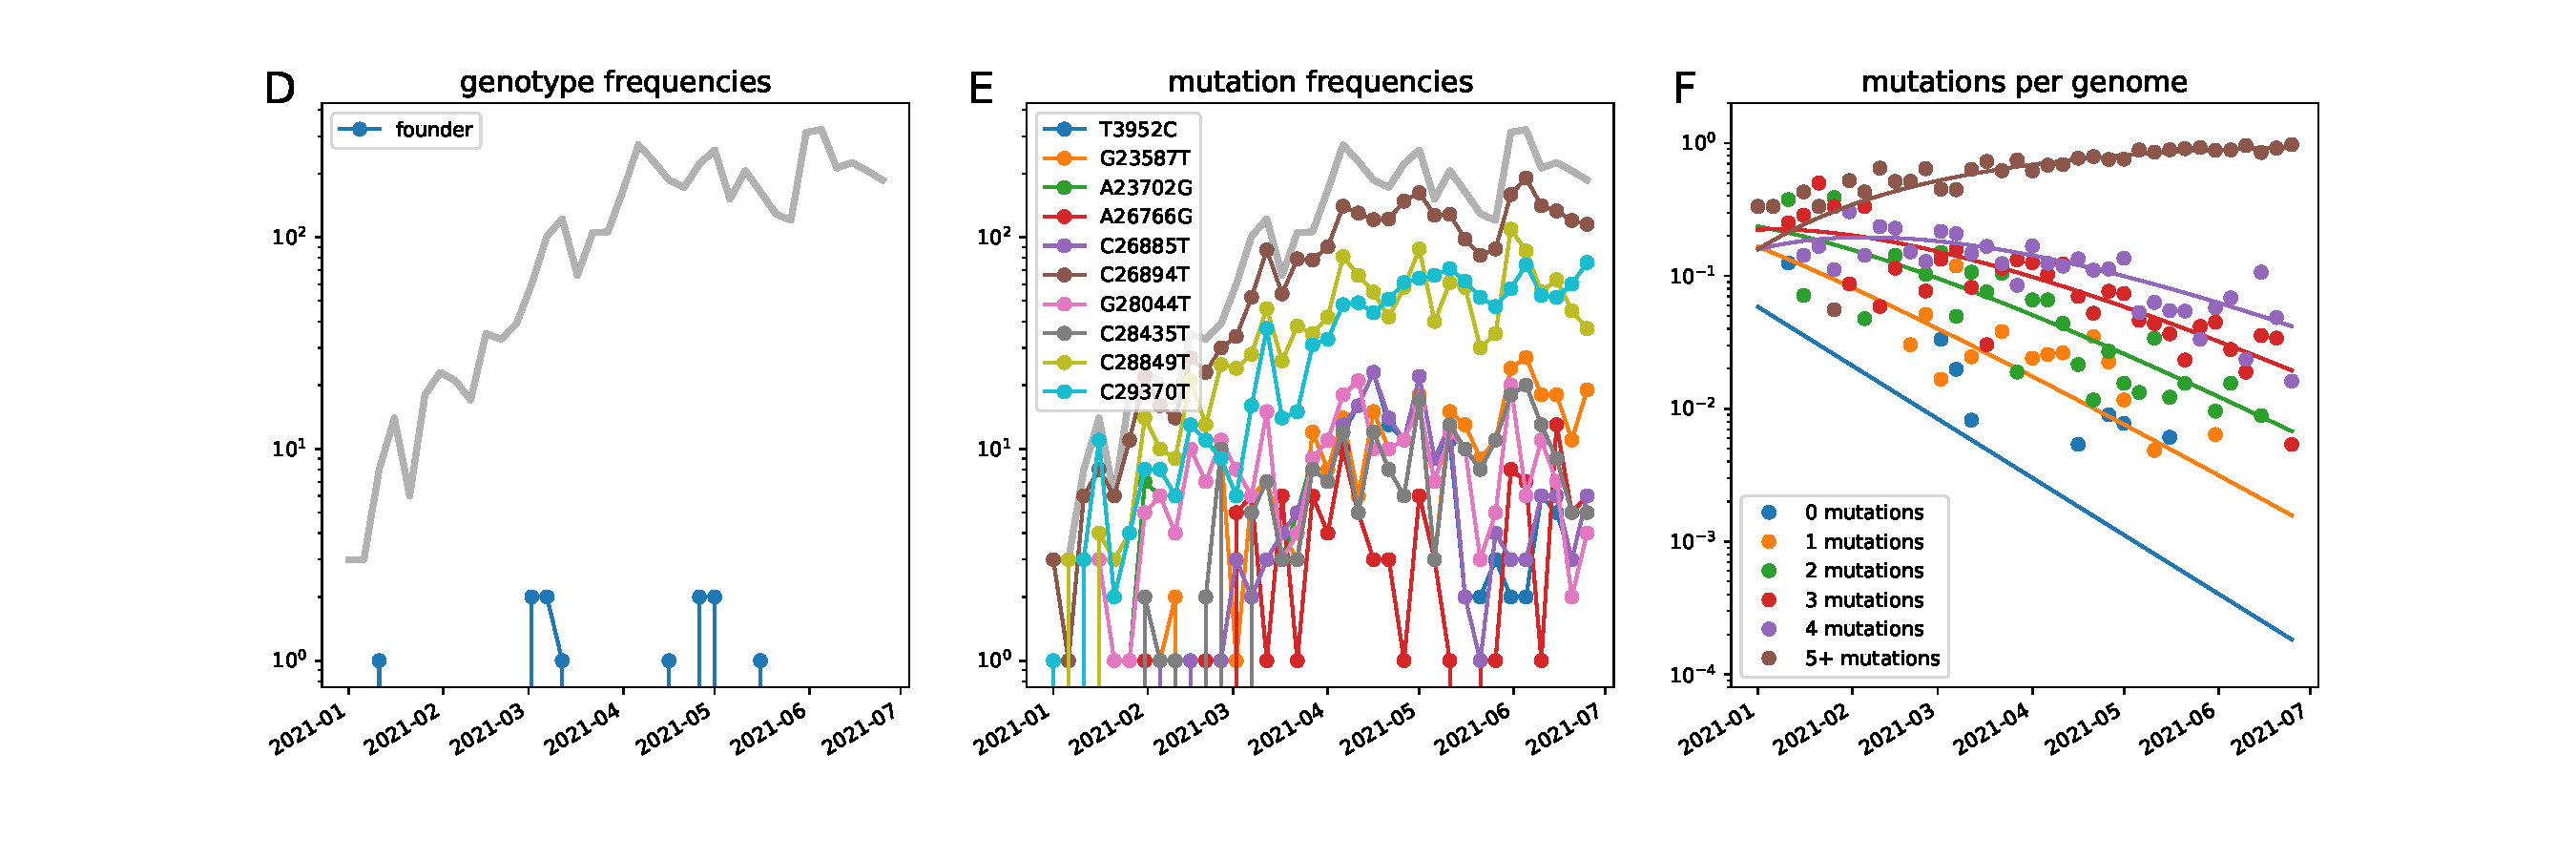
\includegraphics[width=\textwidth]{figures/counts/21G_counts.pdf}
    \caption{{\bf Diversification within clade 21G (Lambda).}
    \label{fig:21G_counts}}
\end{figure*}


\begin{figure*}[h]
    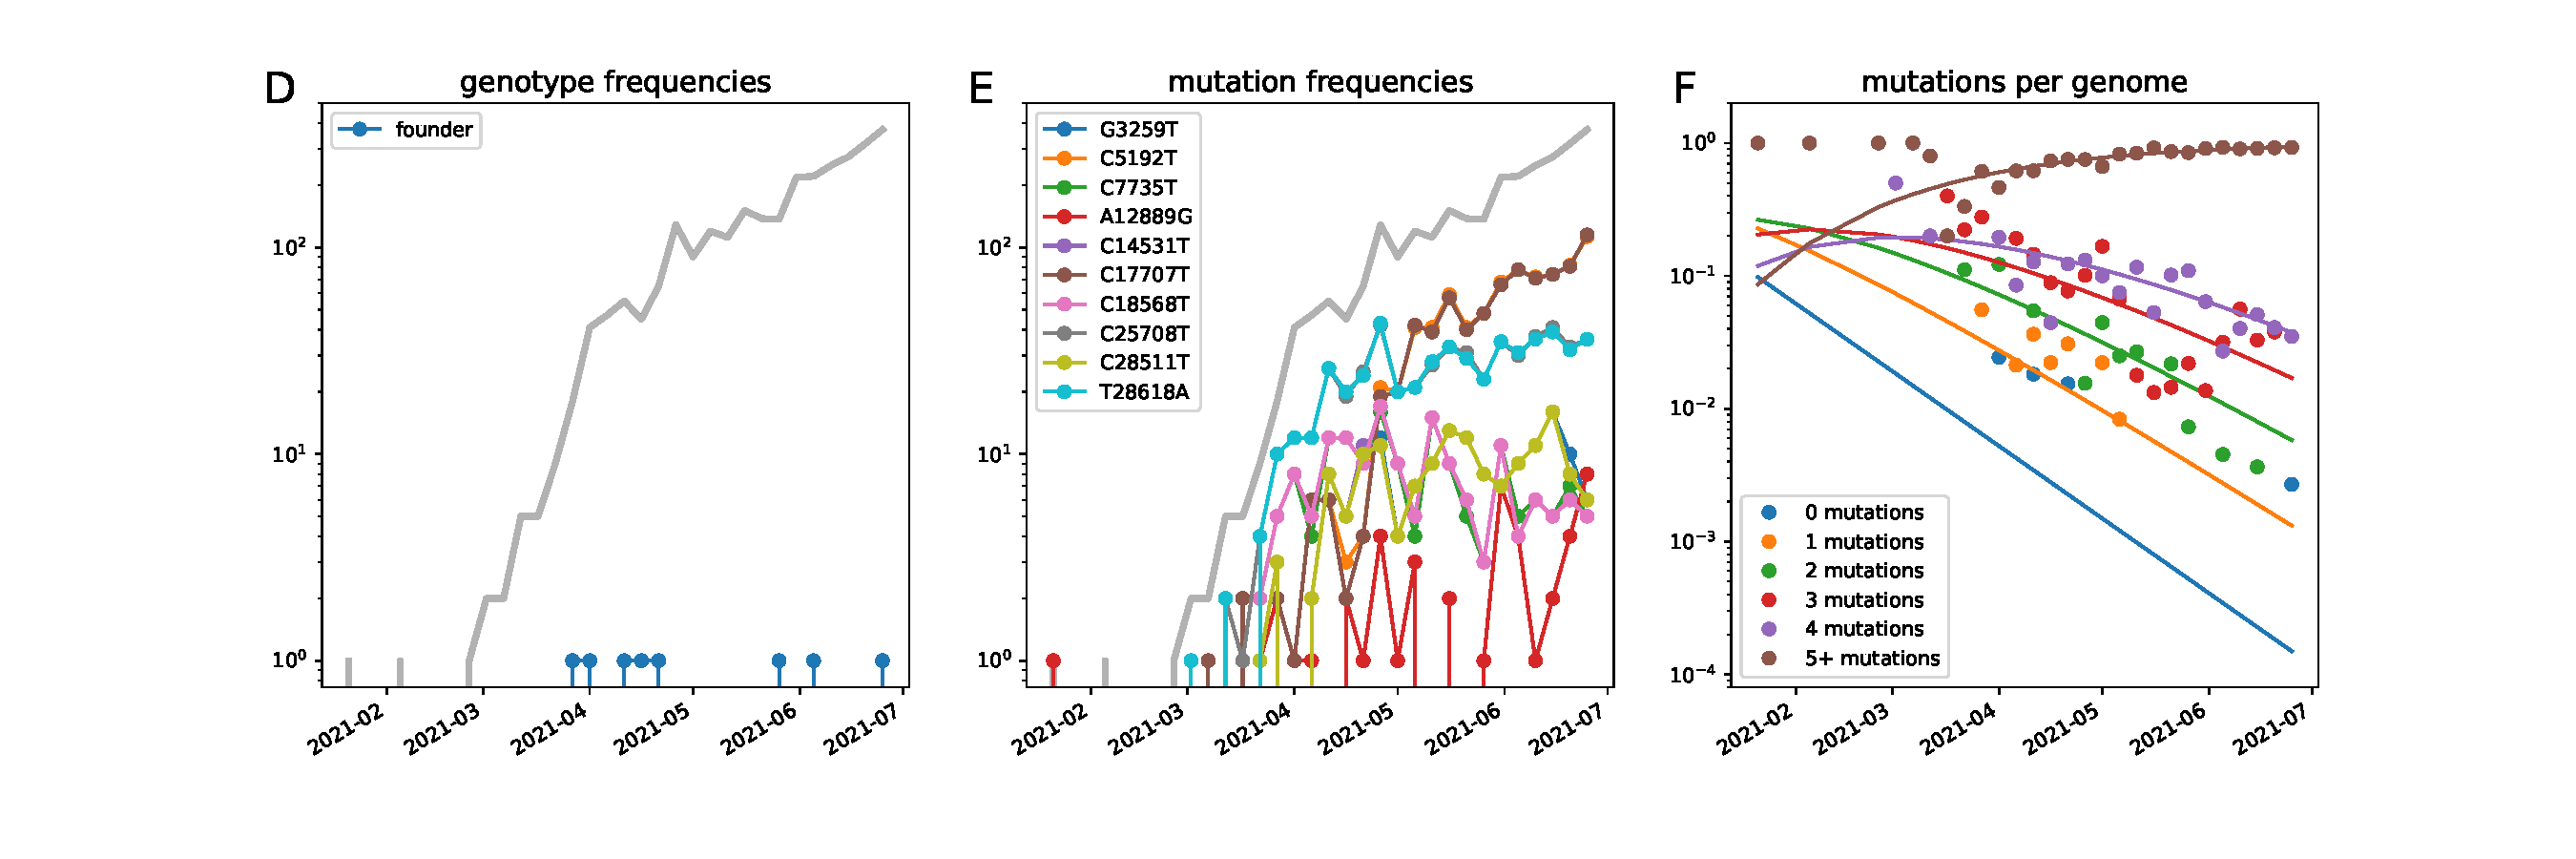
\includegraphics[width=\textwidth]{figures/counts/21H_counts.pdf}
    \caption{{\bf Diversification within clade 21H (Mu).}
    \label{fig:21H_counts}}
\end{figure*}



\begin{figure*}[h]
    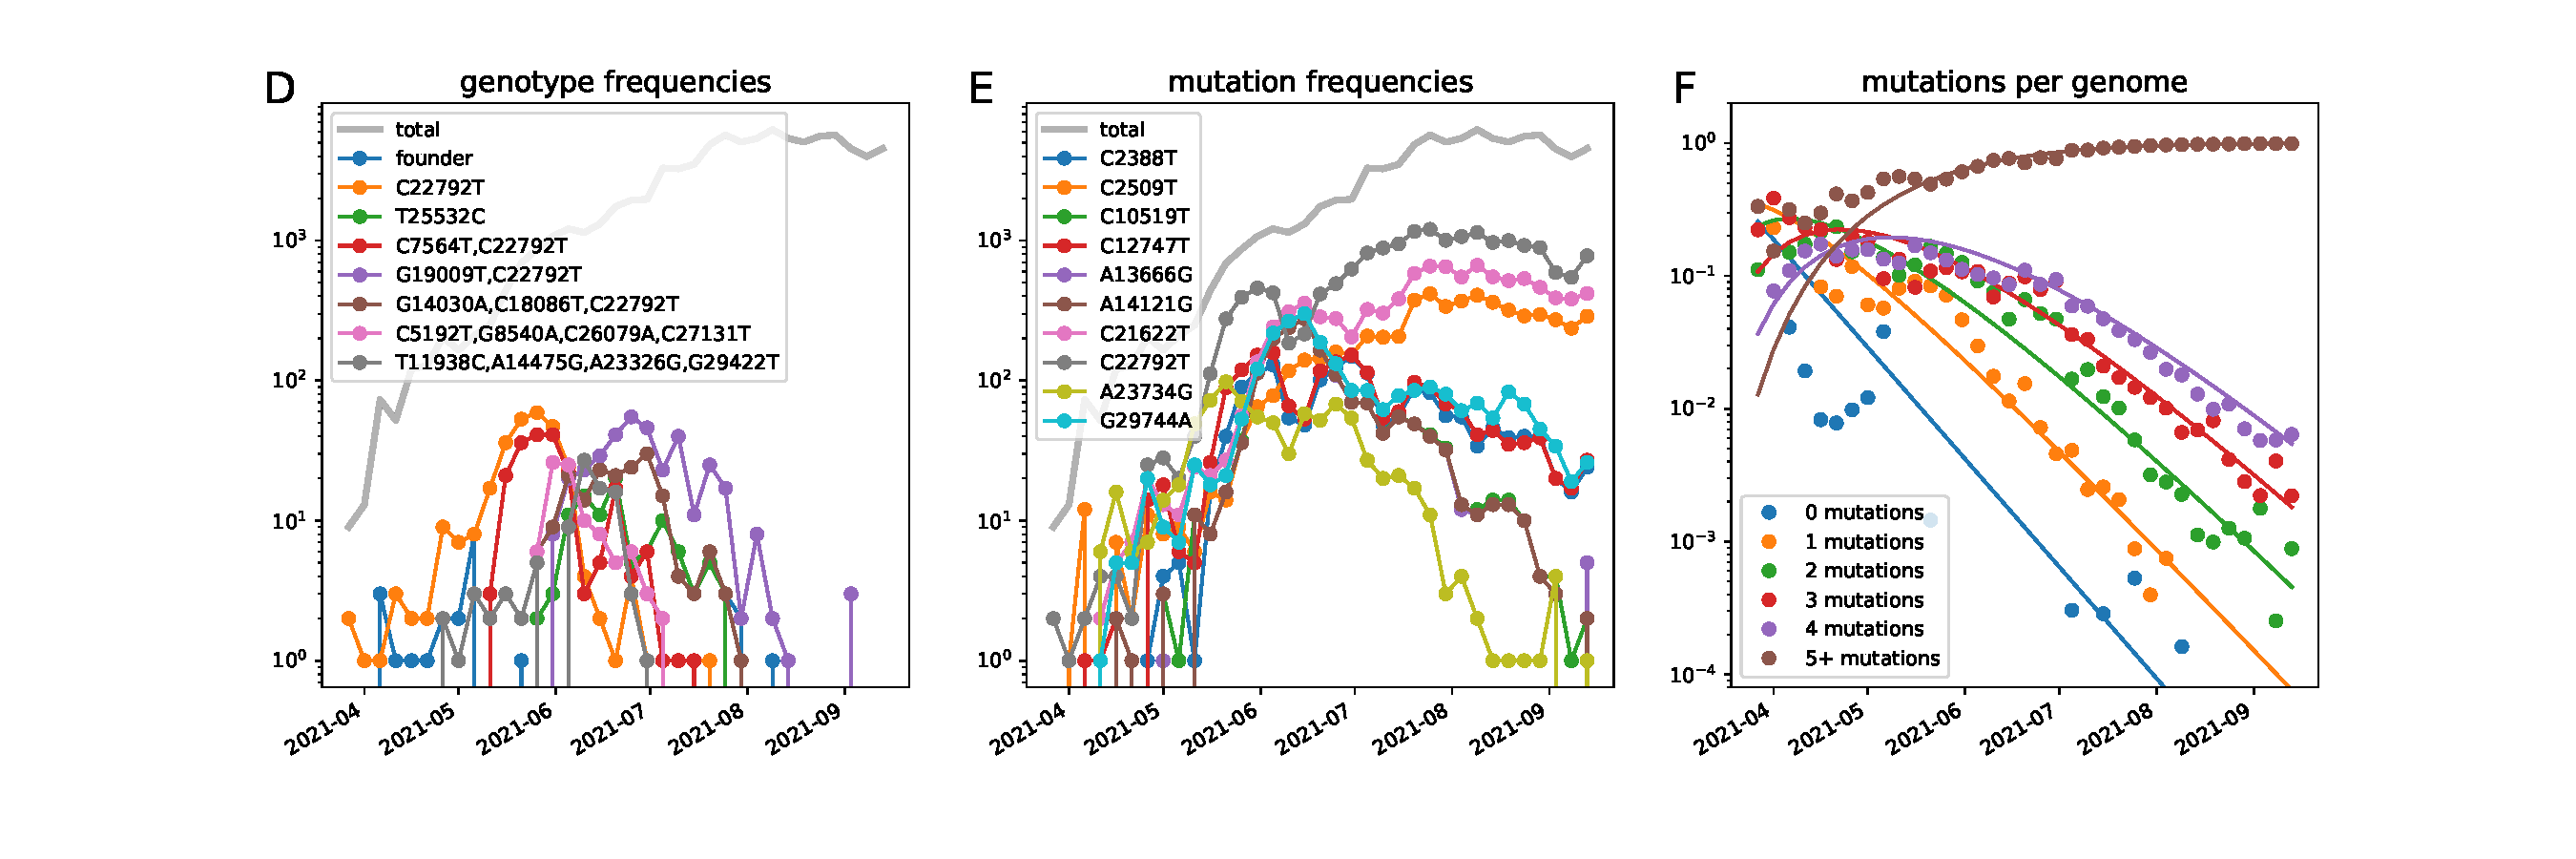
\includegraphics[width=\textwidth]{figures/counts/21I_counts.pdf}
    \caption{{\bf Diversification within clade 21I (Delta).}
    \label{fig:21I_counts}}
\end{figure*}


\begin{figure*}[h]
    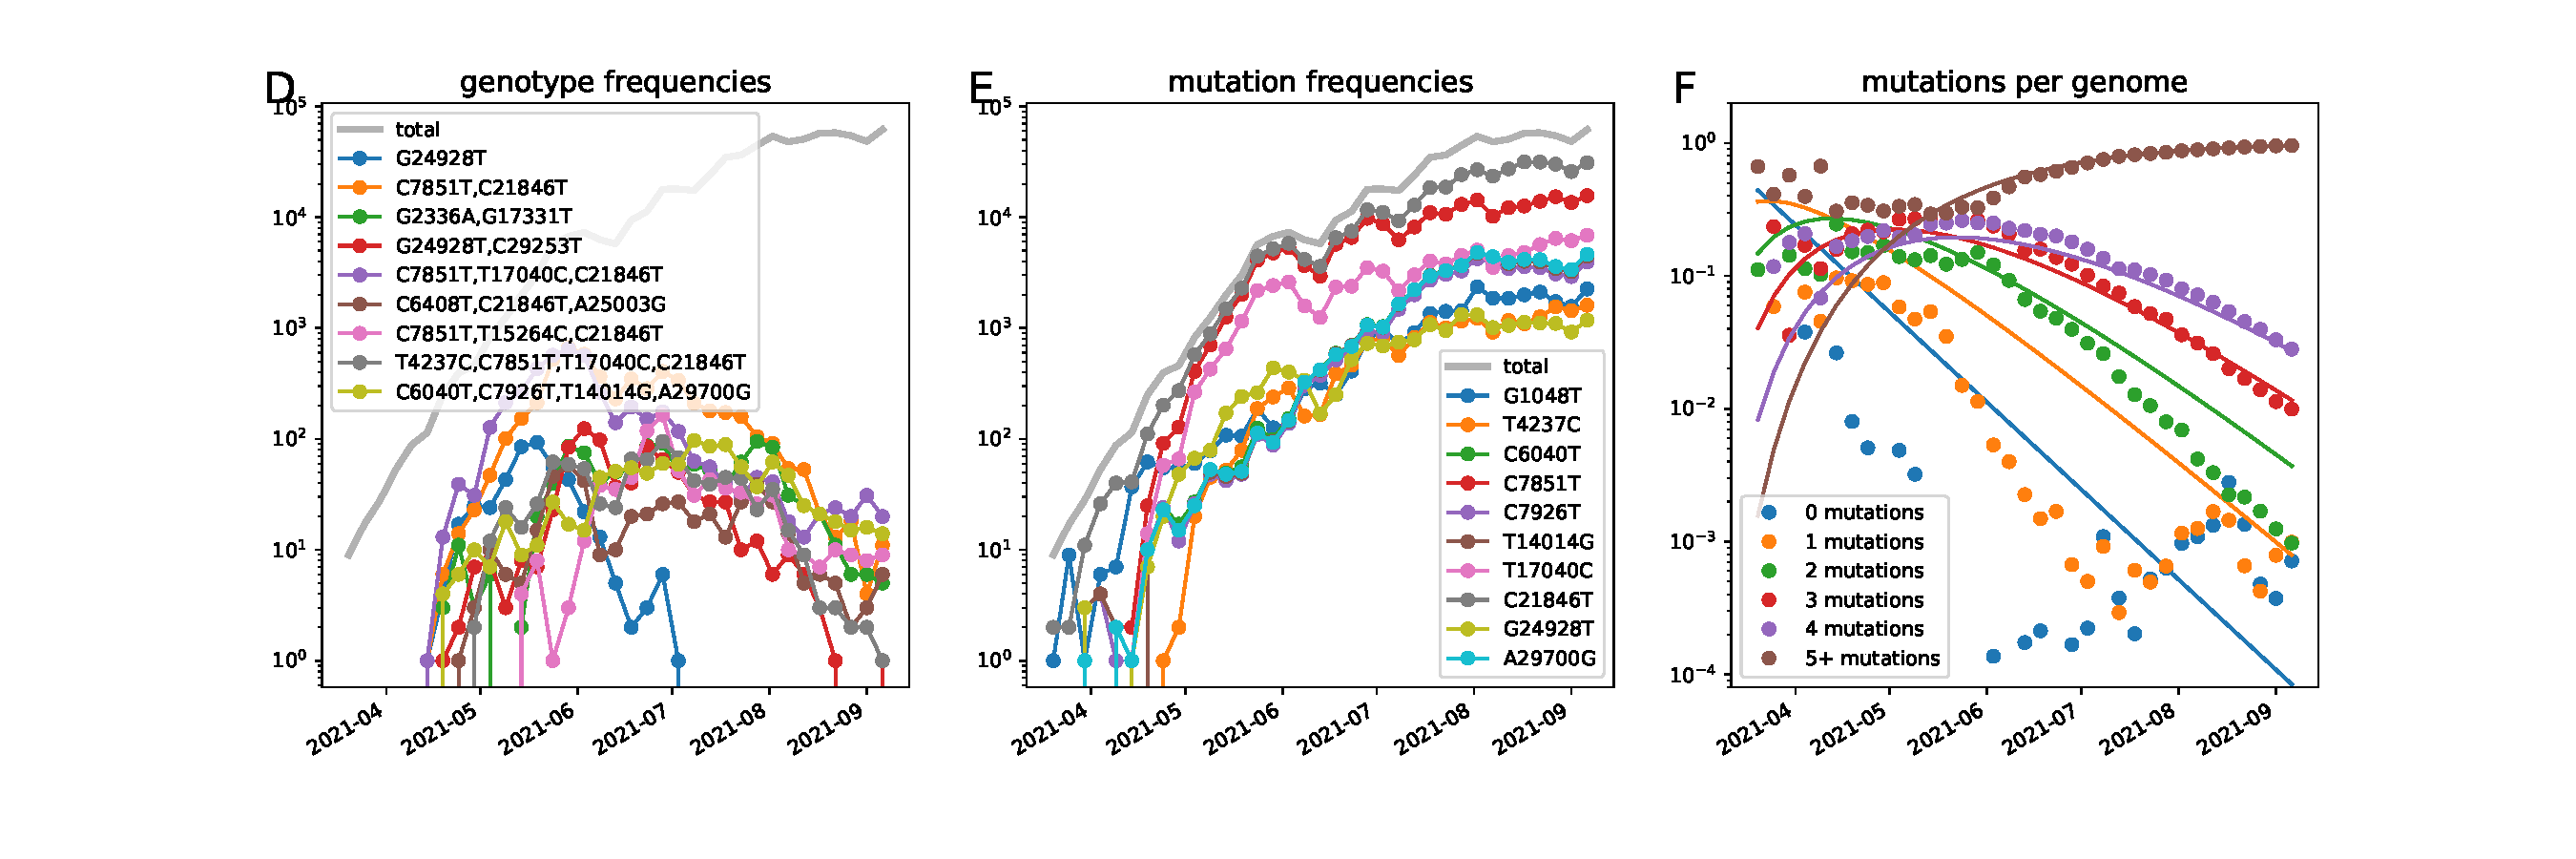
\includegraphics[width=\textwidth]{figures/counts/21J_counts.pdf}
    \caption{{\bf Diversification within clade 21J (Delta).}
    \label{fig:21J_counts}}
\end{figure*}

\begin{figure*}[h]
    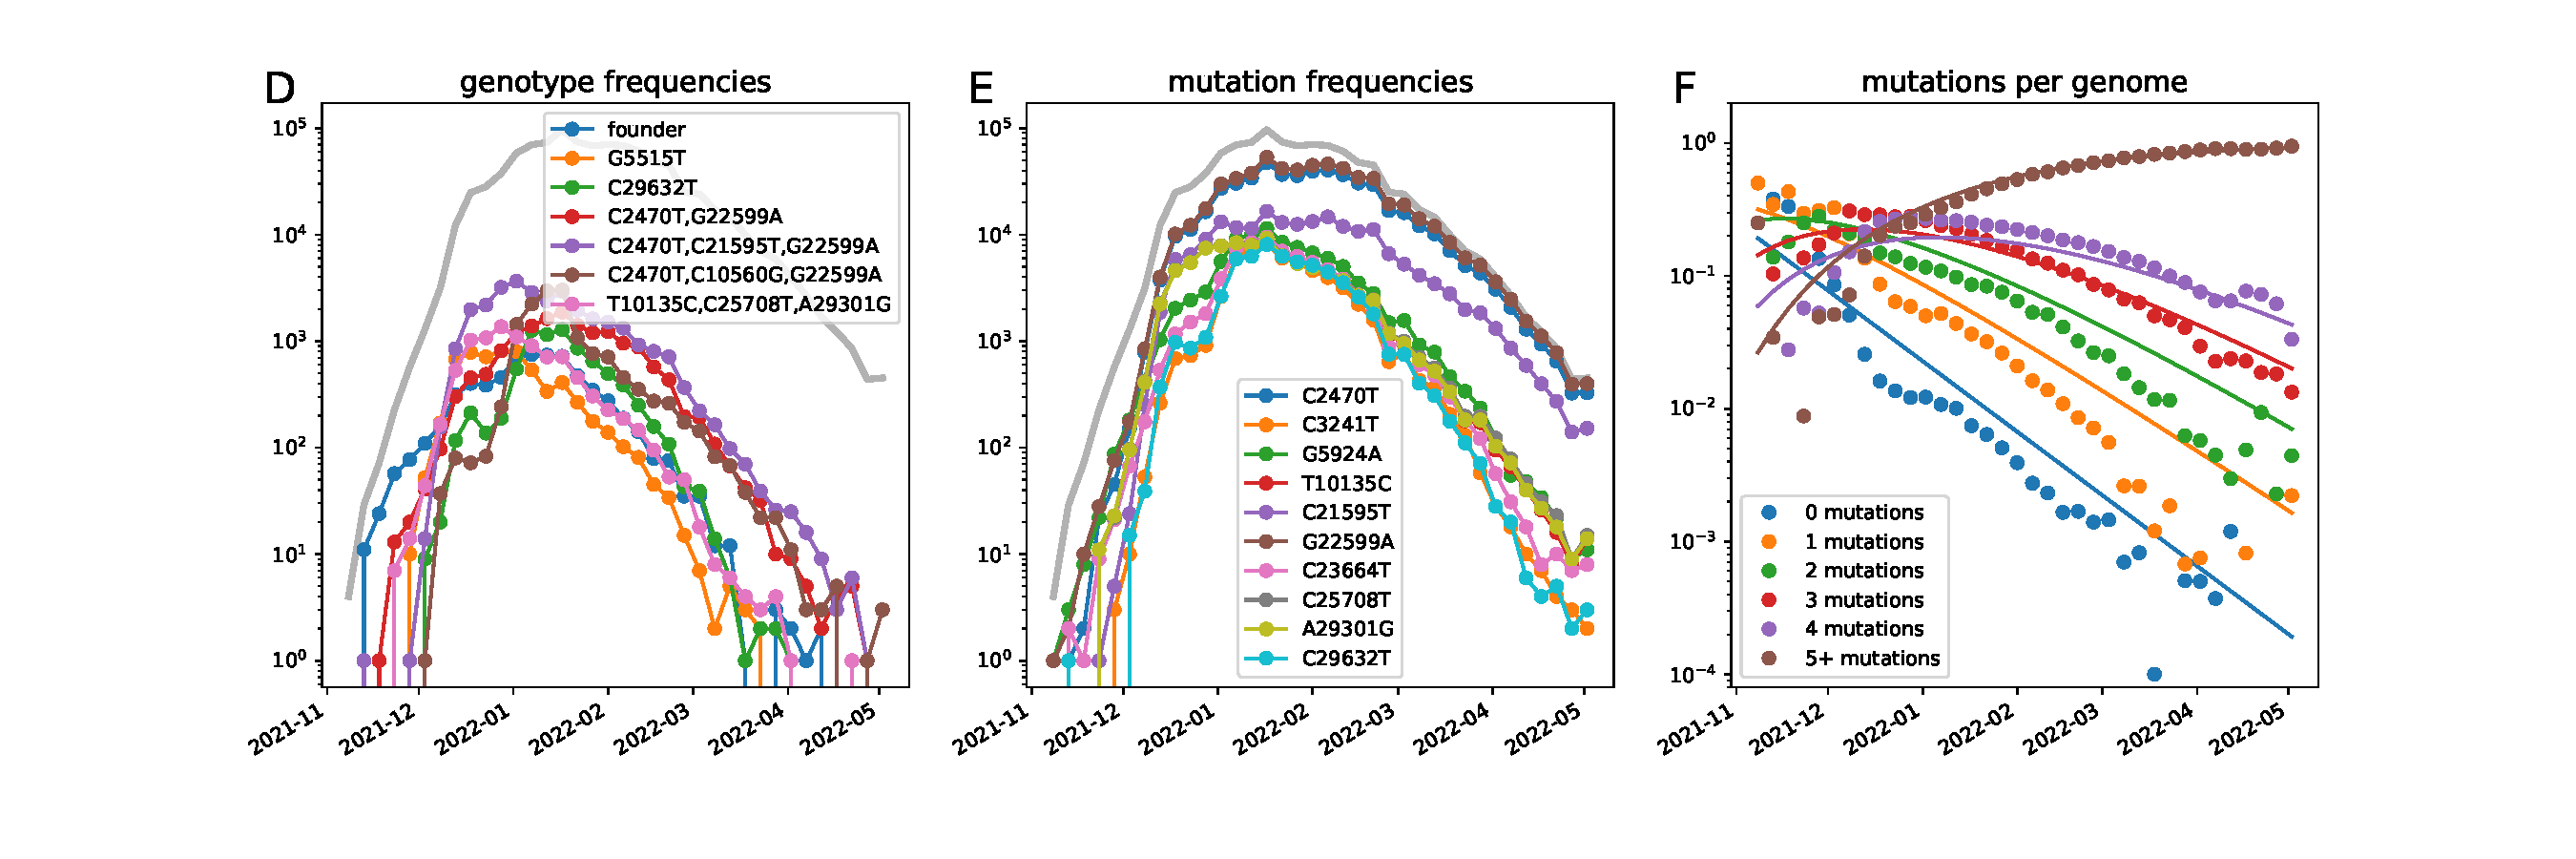
\includegraphics[width=\textwidth]{figures/counts/21K_counts.pdf}
    \caption{{\bf Diversification within clade 21K (Omicron).}
    \label{fig:21K_counts}}
\end{figure*}

\begin{figure*}[h]
    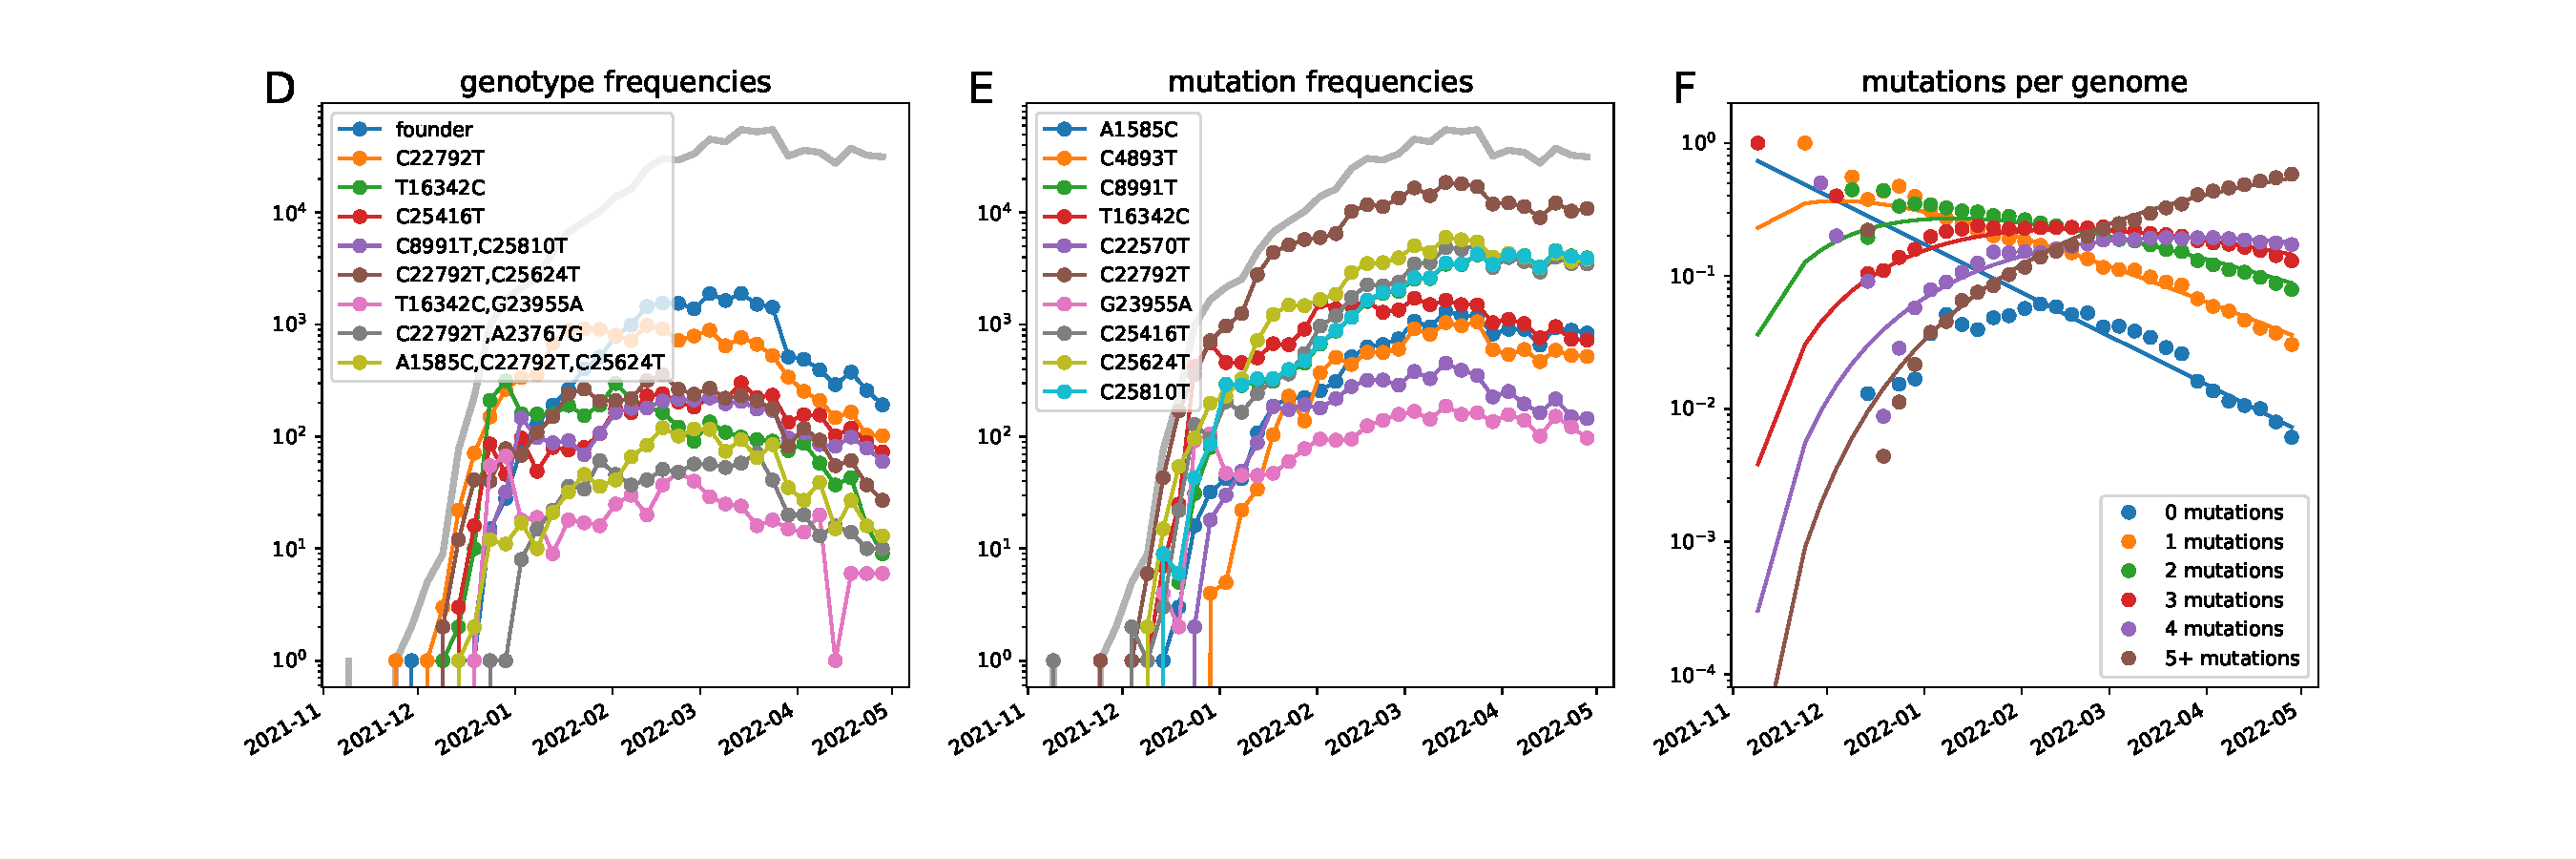
\includegraphics[width=\textwidth]{figures/counts/21L_counts.pdf}
    \caption{{\bf Diversification within clade 21L (Omicron).}
    \label{fig:21L_counts}}
\end{figure*}

\begin{figure*}[h]
    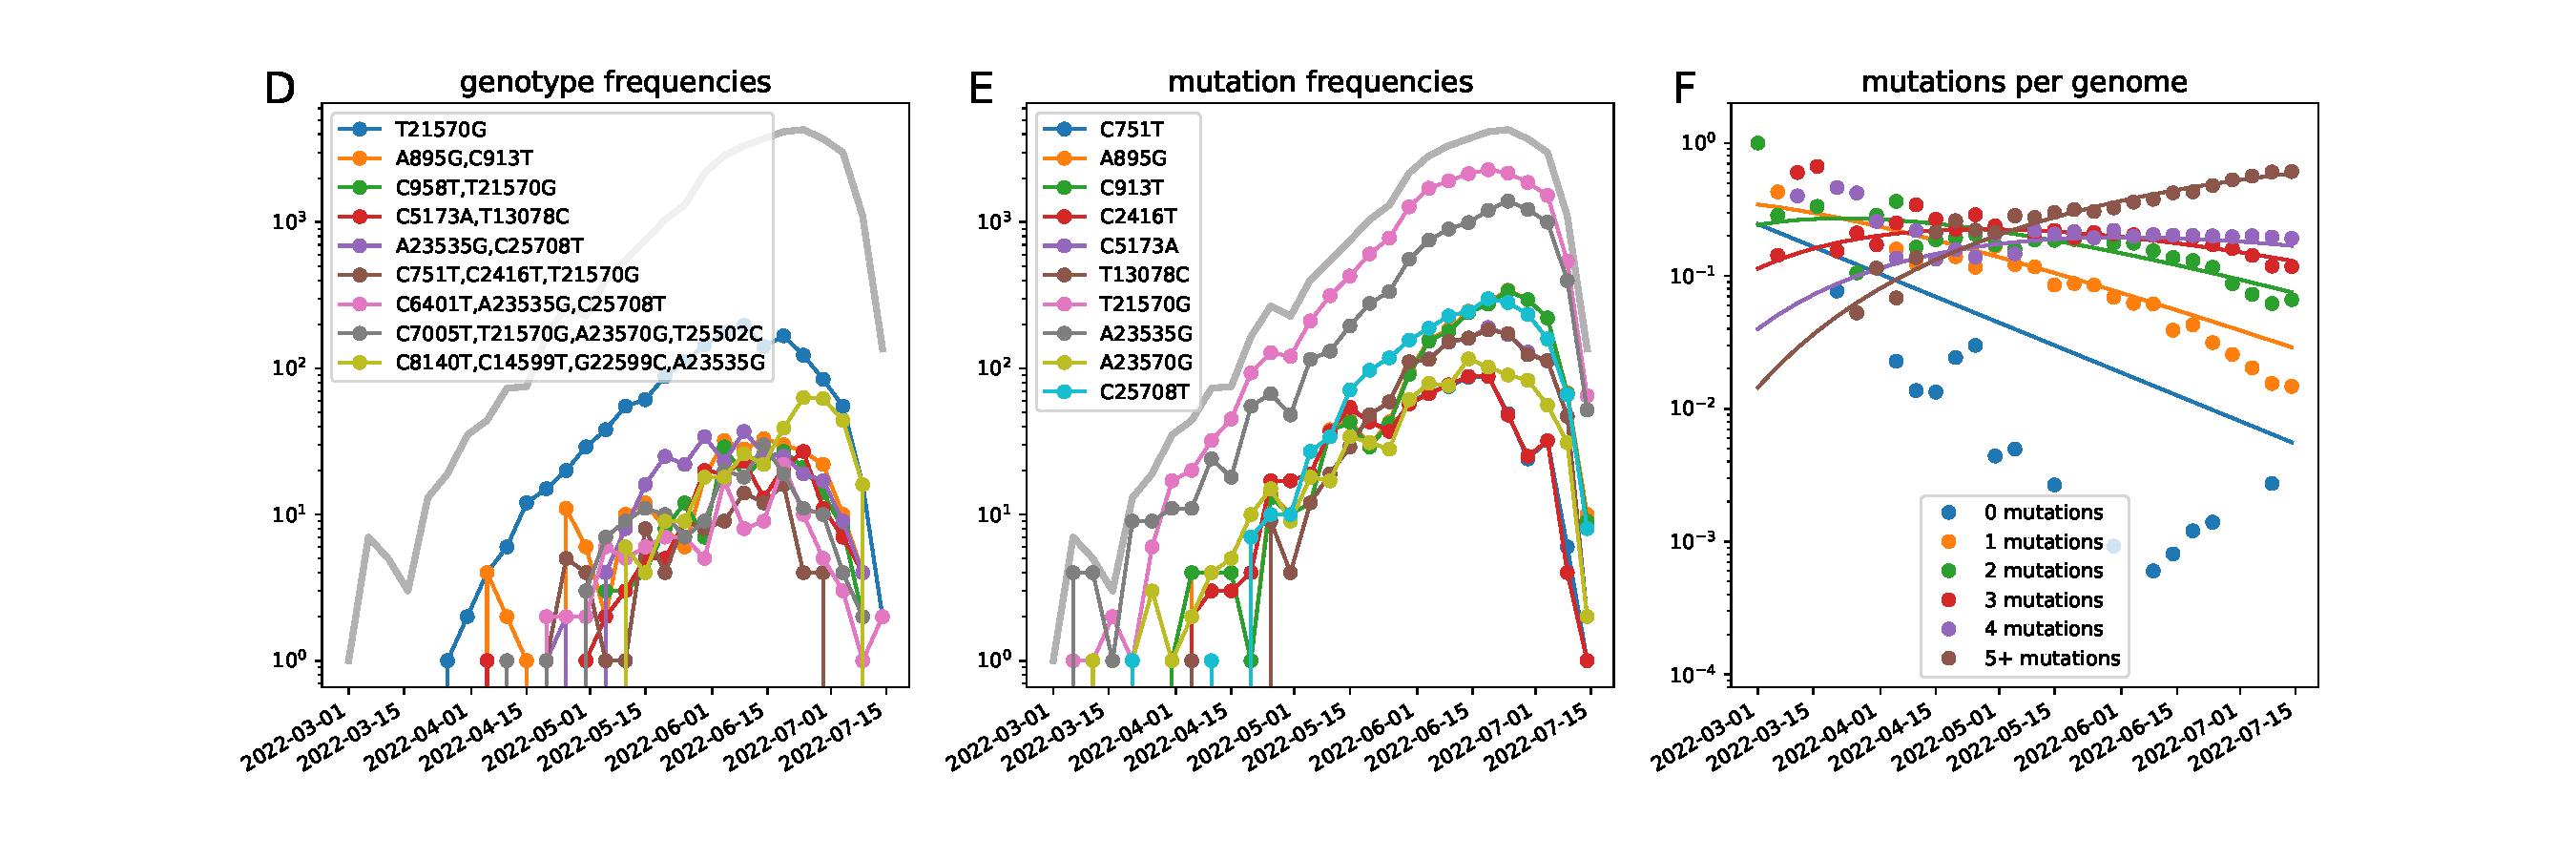
\includegraphics[width=\textwidth]{figures/counts/22A_counts.pdf}
    \caption{{\bf Diversification within clade 22A (Omicron).}
    \label{fig:22A_counts}}
\end{figure*}

\begin{figure*}[h]
    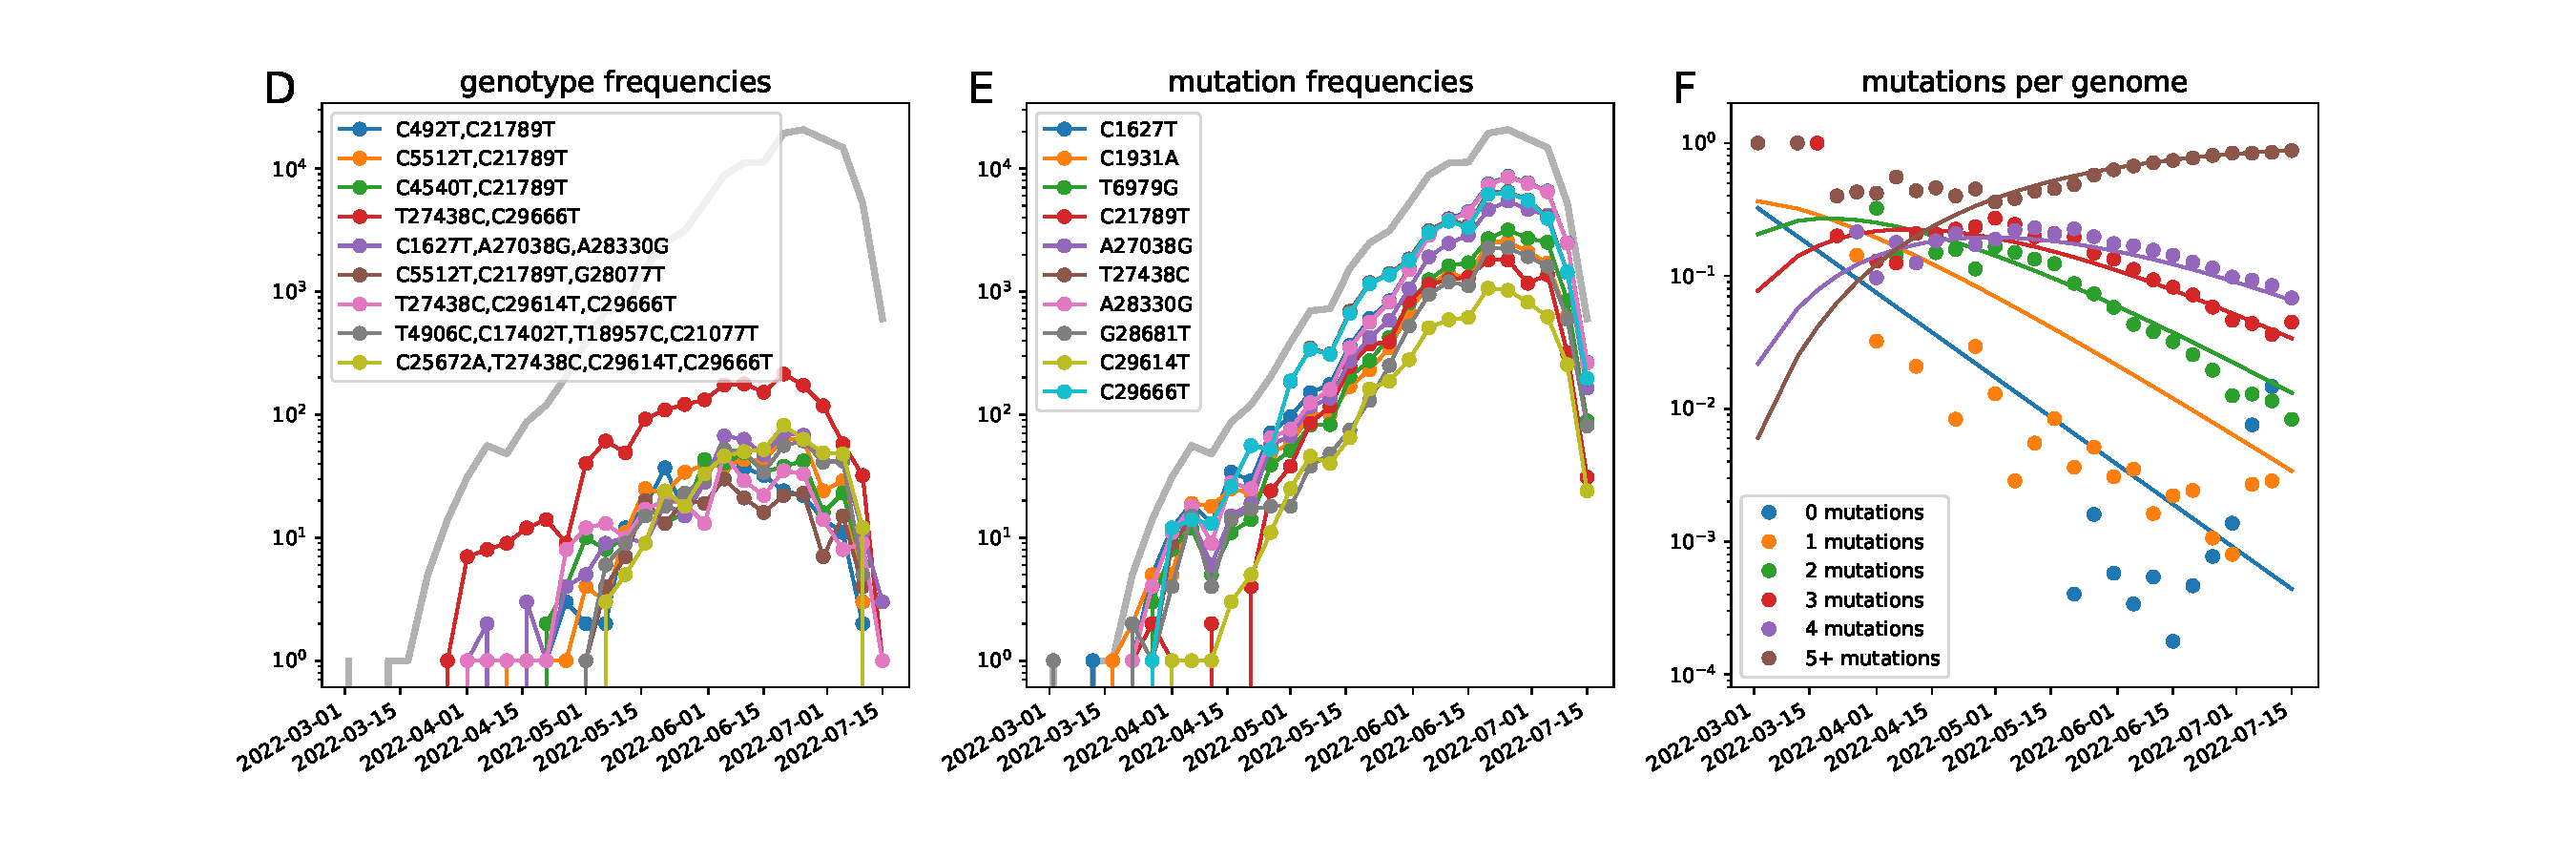
\includegraphics[width=\textwidth]{figures/counts/22B_counts.pdf}
    \caption{{\bf Diversification within clade 22B (Omicron).}
    \label{fig:22B_counts}}
\end{figure*}

\end{document}
